\documentclass[twoside]{book}

% Packages required by doxygen
\usepackage{fixltx2e}
\usepackage{calc}
\usepackage{doxygen}
\usepackage[export]{adjustbox} % also loads graphicx
\usepackage{graphicx}
\usepackage[utf8]{inputenc}
\usepackage{makeidx}
\usepackage{multicol}
\usepackage{multirow}
\PassOptionsToPackage{warn}{textcomp}
\usepackage{textcomp}
\usepackage[nointegrals]{wasysym}
\usepackage[table]{xcolor}

% Font selection
\usepackage[T1]{fontenc}
\usepackage[scaled=.90]{helvet}
\usepackage{courier}
\usepackage{amssymb}
\usepackage{sectsty}
\renewcommand{\familydefault}{\sfdefault}
\allsectionsfont{%
  \fontseries{bc}\selectfont%
  \color{darkgray}%
}
\renewcommand{\DoxyLabelFont}{%
  \fontseries{bc}\selectfont%
  \color{darkgray}%
}
\newcommand{\+}{\discretionary{\mbox{\scriptsize$\hookleftarrow$}}{}{}}

% Page & text layout
\usepackage{geometry}
\geometry{%
  a4paper,%
  top=2.5cm,%
  bottom=2.5cm,%
  left=2.5cm,%
  right=2.5cm%
}
\tolerance=750
\hfuzz=15pt
\hbadness=750
\setlength{\emergencystretch}{15pt}
\setlength{\parindent}{0cm}
\setlength{\parskip}{3ex plus 2ex minus 2ex}
\makeatletter
\renewcommand{\paragraph}{%
  \@startsection{paragraph}{4}{0ex}{-1.0ex}{1.0ex}{%
    \normalfont\normalsize\bfseries\SS@parafont%
  }%
}
\renewcommand{\subparagraph}{%
  \@startsection{subparagraph}{5}{0ex}{-1.0ex}{1.0ex}{%
    \normalfont\normalsize\bfseries\SS@subparafont%
  }%
}
\makeatother

% Headers & footers
\usepackage{fancyhdr}
\pagestyle{fancyplain}
\fancyhead[LE]{\fancyplain{}{\bfseries\thepage}}
\fancyhead[CE]{\fancyplain{}{}}
\fancyhead[RE]{\fancyplain{}{\bfseries\leftmark}}
\fancyhead[LO]{\fancyplain{}{\bfseries\rightmark}}
\fancyhead[CO]{\fancyplain{}{}}
\fancyhead[RO]{\fancyplain{}{\bfseries\thepage}}
\fancyfoot[LE]{\fancyplain{}{}}
\fancyfoot[CE]{\fancyplain{}{}}
\fancyfoot[RE]{\fancyplain{}{\bfseries\scriptsize Generated by Doxygen }}
\fancyfoot[LO]{\fancyplain{}{\bfseries\scriptsize Generated by Doxygen }}
\fancyfoot[CO]{\fancyplain{}{}}
\fancyfoot[RO]{\fancyplain{}{}}
\renewcommand{\footrulewidth}{0.4pt}
\renewcommand{\chaptermark}[1]{%
  \markboth{#1}{}%
}
\renewcommand{\sectionmark}[1]{%
  \markright{\thesection\ #1}%
}

% Indices & bibliography
\usepackage{natbib}
\usepackage[titles]{tocloft}
\setcounter{tocdepth}{3}
\setcounter{secnumdepth}{5}
\makeindex

% Hyperlinks (required, but should be loaded last)
\usepackage{ifpdf}
\ifpdf
  \usepackage[pdftex,pagebackref=true]{hyperref}
\else
  \usepackage[ps2pdf,pagebackref=true]{hyperref}
\fi
\hypersetup{%
  colorlinks=true,%
  linkcolor=blue,%
  citecolor=blue,%
  unicode%
}

% Custom commands
\newcommand{\clearemptydoublepage}{%
  \newpage{\pagestyle{empty}\cleardoublepage}%
}

\usepackage{caption}
\captionsetup{labelsep=space,justification=centering,font={bf},singlelinecheck=off,skip=4pt,position=top}

%===== C O N T E N T S =====

\begin{document}

% Titlepage & ToC
\hypersetup{pageanchor=false,
             bookmarksnumbered=true,
             pdfencoding=unicode
            }
\pagenumbering{alph}
\begin{titlepage}
\vspace*{7cm}
\begin{center}%
{\Large My Project }\\
\vspace*{1cm}
{\large Generated by Doxygen 1.8.14}\\
\end{center}
\end{titlepage}
\clearemptydoublepage
\pagenumbering{roman}
\tableofcontents
\clearemptydoublepage
\pagenumbering{arabic}
\hypersetup{pageanchor=true}

%--- Begin generated contents ---
\chapter{Namespace Index}
\doxysection{Packages}
Here are the packages with brief descriptions (if available)\+:\begin{DoxyCompactList}
\item\contentsline{section}{\mbox{\hyperlink{namespaceopenbu_1_1passlist}{openbu.\+passlist}} }{\pageref{namespaceopenbu_1_1passlist}}{}
\item\contentsline{section}{\mbox{\hyperlink{namespaceopenbu_1_1passport}{openbu.\+passport}} }{\pageref{namespaceopenbu_1_1passport}}{}
\item\contentsline{section}{\mbox{\hyperlink{namespaceopenbu_1_1salameche_1_1cram}{openbu.\+salameche.\+cram}} }{\pageref{namespaceopenbu_1_1salameche_1_1cram}}{}
\item\contentsline{section}{\mbox{\hyperlink{namespaceopenbu_1_1salameche_1_1mat__builder}{openbu.\+salameche.\+mat\+\_\+builder}} }{\pageref{namespaceopenbu_1_1salameche_1_1mat__builder}}{}
\item\contentsline{section}{\mbox{\hyperlink{namespaceopenbu_1_1utils_1_1reactions__class}{openbu.\+utils.\+reactions\+\_\+class}} }{\pageref{namespaceopenbu_1_1utils_1_1reactions__class}}{}
\end{DoxyCompactList}

\chapter{Design Unit Index}
\doxysection{Design Unit Hierarchy}
Here is a hierarchical list of all entities\+:\begin{DoxyCompactList}
\item Exception\begin{DoxyCompactList}
\item \contentsline{section}{Initial\+\_\+nucl\+\_\+not\+\_\+in\+\_\+\+Nucl\+\_\+set}{\pageref{classopenbu_1_1cell_1_1_initial__nucl__not__in___nucl__set}}{}
\item \contentsline{section}{Initial\+\_\+nucl\+\_\+not\+\_\+set}{\pageref{classopenbu_1_1cell_1_1_initial__nucl__not__set}}{}
\item \contentsline{section}{Nucl\+\_\+set\+\_\+not\+\_\+in\+\_\+\+Lib\+\_\+nucl}{\pageref{classopenbu_1_1cell_1_1_nucl__set__not__in___lib__nucl}}{}
\item \contentsline{section}{Nuclide\+\_\+list\+\_\+redundant}{\pageref{classopenbu_1_1cell_1_1_nuclide__list__redundant}}{}
\item \contentsline{section}{Passlist\+\_\+not\+\_\+defined}{\pageref{classopenbu_1_1cell_1_1_passlist__not__defined}}{}
\item \contentsline{section}{Initial\+\_\+nuclides\+\_\+not\+\_\+in\+\_\+nuclide\+\_\+list}{\pageref{classopenbu_1_1couple_1_1couple__openmc_1_1_initial__nuclides__not__in__nuclide__list}}{}
\item \contentsline{section}{S\+T\+OP}{\pageref{classopenbu_1_1couple_1_1couple__openmc_1_1_s_t_o_p}}{}
\item \contentsline{section}{Neg\+\_\+decay}{\pageref{classopenbu_1_1passlist_1_1_neg__decay}}{}
\item \contentsline{section}{Neg\+\_\+xs}{\pageref{classopenbu_1_1passlist_1_1_neg__xs}}{}
\item \contentsline{section}{Nuc\+\_\+xs\+\_\+not\+\_\+found}{\pageref{classopenbu_1_1passlist_1_1_nuc__xs__not__found}}{}
\item \contentsline{section}{Incorrect\+\_\+nuc\+\_\+id}{\pageref{classopenbu_1_1passport_1_1_incorrect__nuc__id}}{}
\item \contentsline{section}{No\+\_\+fission\+\_\+\+XS}{\pageref{classopenbu_1_1passport_1_1_no__fission___x_s}}{}
\item \contentsline{section}{Not\+\_\+a\+\_\+\+Fission\+\_\+\+Product}{\pageref{classopenbu_1_1passport_1_1_not__a___fission___product}}{}
\item \contentsline{section}{Nuc\+\_\+xs\+\_\+not\+\_\+found}{\pageref{classopenbu_1_1passport_1_1_nuc__xs__not__found}}{}
\item \contentsline{section}{X\+S\+\_\+not\+\_\+yet\+\_\+set}{\pageref{classopenbu_1_1passport_1_1_x_s__not__yet__set}}{}
\item \contentsline{section}{Step\+\_\+0}{\pageref{classopenbu_1_1sequence_1_1_step__0}}{}
\item \contentsline{section}{Cell\+\_\+name\+\_\+not\+\_\+found}{\pageref{classopenbu_1_1system_1_1_cell__name__not__found}}{}
\item \contentsline{section}{xs\+\_\+name\+\_\+not\+\_\+found}{\pageref{classopenbu_1_1utils_1_1data__processor_1_1xs__name__not__found}}{}
\item \contentsline{section}{Empty\+\_\+argument}{\pageref{classopenbu_1_1utils_1_1functions_1_1_empty__argument}}{}
\item \contentsline{section}{Empty\+\_\+data}{\pageref{classopenbu_1_1utils_1_1reactions__class_1_1_empty__data}}{}
\end{DoxyCompactList}
\item Normalize\begin{DoxyCompactList}
\item \contentsline{section}{Midpoint\+Normalize}{\pageref{classopenbu_1_1utils_1_1functions_1_1_midpoint_normalize}}{}
\end{DoxyCompactList}
\item object\begin{DoxyCompactList}
\item \contentsline{section}{Cell}{\pageref{classopenbu_1_1cell_1_1_cell}}{}
\item \contentsline{section}{Couple\+\_\+openmc}{\pageref{classopenbu_1_1couple_1_1couple__openmc_1_1_couple__openmc}}{}
\item \contentsline{section}{Input}{\pageref{classopenbu_1_1input_1_1_input}}{}
\item \contentsline{section}{Batch}{\pageref{classopenbu_1_1nax_1_1functions_1_1_batch}}{}
\item \contentsline{section}{Passlist}{\pageref{classopenbu_1_1passlist_1_1_passlist}}{}
\item \contentsline{section}{Passport}{\pageref{classopenbu_1_1passport_1_1_passport}}{}
\item \contentsline{section}{Sequence}{\pageref{classopenbu_1_1sequence_1_1_sequence}}{}
\item \contentsline{section}{Stand\+\_\+alone}{\pageref{classopenbu_1_1standalone_1_1_stand__alone}}{}
\item \contentsline{section}{System}{\pageref{classopenbu_1_1system_1_1_system}}{}
\item \contentsline{section}{decay\+\_\+lib}{\pageref{classopenbu_1_1utils_1_1reactions__class_1_1decay__lib}}{}
\item \contentsline{section}{fy\+\_\+lib}{\pageref{classopenbu_1_1utils_1_1reactions__class_1_1fy__lib}}{}
\item \contentsline{section}{xs\+\_\+lib}{\pageref{classopenbu_1_1utils_1_1reactions__class_1_1xs__lib}}{}
\end{DoxyCompactList}
\end{DoxyCompactList}

\chapter{Design Unit Index}
\doxysection{Design Unit List}
Here is a list of all design unit members with links to the Entities they belong to\+:\begin{DoxyCompactList}
\item\contentsline{section}{\mbox{\hyperlink{classopenbu_1_1nax_1_1functions_1_1_batch}{Batch}} }{\pageref{classopenbu_1_1nax_1_1functions_1_1_batch}}{}
\item\contentsline{section}{\mbox{\hyperlink{classopenbu_1_1cell_1_1_cell}{Cell}} }{\pageref{classopenbu_1_1cell_1_1_cell}}{}
\item\contentsline{section}{\mbox{\hyperlink{classopenbu_1_1system_1_1_cell__name__not__found}{Cell\+\_\+name\+\_\+not\+\_\+found}} }{\pageref{classopenbu_1_1system_1_1_cell__name__not__found}}{}
\item\contentsline{section}{\mbox{\hyperlink{classopenbu_1_1couple_1_1couple__openmc_1_1_couple__openmc}{Couple\+\_\+openmc}} }{\pageref{classopenbu_1_1couple_1_1couple__openmc_1_1_couple__openmc}}{}
\item\contentsline{section}{\mbox{\hyperlink{classopenbu_1_1utils_1_1reactions__class_1_1decay__lib}{decay\+\_\+lib}} }{\pageref{classopenbu_1_1utils_1_1reactions__class_1_1decay__lib}}{}
\item\contentsline{section}{\mbox{\hyperlink{classopenbu_1_1utils_1_1functions_1_1_empty__argument}{Empty\+\_\+argument}} }{\pageref{classopenbu_1_1utils_1_1functions_1_1_empty__argument}}{}
\item\contentsline{section}{\mbox{\hyperlink{classopenbu_1_1utils_1_1reactions__class_1_1_empty__data}{Empty\+\_\+data}} }{\pageref{classopenbu_1_1utils_1_1reactions__class_1_1_empty__data}}{}
\item\contentsline{section}{\mbox{\hyperlink{classopenbu_1_1utils_1_1reactions__class_1_1fy__lib}{fy\+\_\+lib}} }{\pageref{classopenbu_1_1utils_1_1reactions__class_1_1fy__lib}}{}
\item\contentsline{section}{\mbox{\hyperlink{classopenbu_1_1passport_1_1_incorrect__nuc__id}{Incorrect\+\_\+nuc\+\_\+id}} }{\pageref{classopenbu_1_1passport_1_1_incorrect__nuc__id}}{}
\item\contentsline{section}{\mbox{\hyperlink{classopenbu_1_1cell_1_1_initial__nucl__not__in___nucl__set}{Initial\+\_\+nucl\+\_\+not\+\_\+in\+\_\+\+Nucl\+\_\+set}} }{\pageref{classopenbu_1_1cell_1_1_initial__nucl__not__in___nucl__set}}{}
\item\contentsline{section}{\mbox{\hyperlink{classopenbu_1_1cell_1_1_initial__nucl__not__set}{Initial\+\_\+nucl\+\_\+not\+\_\+set}} }{\pageref{classopenbu_1_1cell_1_1_initial__nucl__not__set}}{}
\item\contentsline{section}{\mbox{\hyperlink{classopenbu_1_1couple_1_1couple__openmc_1_1_initial__nuclides__not__in__nuclide__list}{Initial\+\_\+nuclides\+\_\+not\+\_\+in\+\_\+nuclide\+\_\+list}} }{\pageref{classopenbu_1_1couple_1_1couple__openmc_1_1_initial__nuclides__not__in__nuclide__list}}{}
\item\contentsline{section}{\mbox{\hyperlink{classopenbu_1_1input_1_1_input}{Input}} }{\pageref{classopenbu_1_1input_1_1_input}}{}
\item\contentsline{section}{\mbox{\hyperlink{classopenbu_1_1utils_1_1functions_1_1_midpoint_normalize}{Midpoint\+Normalize}} }{\pageref{classopenbu_1_1utils_1_1functions_1_1_midpoint_normalize}}{}
\item\contentsline{section}{\mbox{\hyperlink{classopenbu_1_1passlist_1_1_neg__decay}{Neg\+\_\+decay}} }{\pageref{classopenbu_1_1passlist_1_1_neg__decay}}{}
\item\contentsline{section}{\mbox{\hyperlink{classopenbu_1_1passlist_1_1_neg__xs}{Neg\+\_\+xs}} }{\pageref{classopenbu_1_1passlist_1_1_neg__xs}}{}
\item\contentsline{section}{\mbox{\hyperlink{classopenbu_1_1passport_1_1_no__fission___x_s}{No\+\_\+fission\+\_\+\+XS}} }{\pageref{classopenbu_1_1passport_1_1_no__fission___x_s}}{}
\item\contentsline{section}{\mbox{\hyperlink{classopenbu_1_1passport_1_1_not__a___fission___product}{Not\+\_\+a\+\_\+\+Fission\+\_\+\+Product}} }{\pageref{classopenbu_1_1passport_1_1_not__a___fission___product}}{}
\item\contentsline{section}{\mbox{\hyperlink{classopenbu_1_1passport_1_1_nuc__xs__not__found}{Nuc\+\_\+xs\+\_\+not\+\_\+found}} }{\pageref{classopenbu_1_1passport_1_1_nuc__xs__not__found}}{}
\item\contentsline{section}{\mbox{\hyperlink{classopenbu_1_1passlist_1_1_nuc__xs__not__found}{Nuc\+\_\+xs\+\_\+not\+\_\+found}} }{\pageref{classopenbu_1_1passlist_1_1_nuc__xs__not__found}}{}
\item\contentsline{section}{\mbox{\hyperlink{classopenbu_1_1cell_1_1_nucl__set__not__in___lib__nucl}{Nucl\+\_\+set\+\_\+not\+\_\+in\+\_\+\+Lib\+\_\+nucl}} }{\pageref{classopenbu_1_1cell_1_1_nucl__set__not__in___lib__nucl}}{}
\item\contentsline{section}{\mbox{\hyperlink{classopenbu_1_1cell_1_1_nuclide__list__redundant}{Nuclide\+\_\+list\+\_\+redundant}} }{\pageref{classopenbu_1_1cell_1_1_nuclide__list__redundant}}{}
\item\contentsline{section}{\mbox{\hyperlink{classopenbu_1_1passlist_1_1_passlist}{Passlist}} }{\pageref{classopenbu_1_1passlist_1_1_passlist}}{}
\item\contentsline{section}{\mbox{\hyperlink{classopenbu_1_1cell_1_1_passlist__not__defined}{Passlist\+\_\+not\+\_\+defined}} }{\pageref{classopenbu_1_1cell_1_1_passlist__not__defined}}{}
\item\contentsline{section}{\mbox{\hyperlink{classopenbu_1_1passport_1_1_passport}{Passport}} }{\pageref{classopenbu_1_1passport_1_1_passport}}{}
\item\contentsline{section}{\mbox{\hyperlink{classopenbu_1_1sequence_1_1_sequence}{Sequence}} }{\pageref{classopenbu_1_1sequence_1_1_sequence}}{}
\item\contentsline{section}{\mbox{\hyperlink{classopenbu_1_1standalone_1_1_stand__alone}{Stand\+\_\+alone}} }{\pageref{classopenbu_1_1standalone_1_1_stand__alone}}{}
\item\contentsline{section}{\mbox{\hyperlink{classopenbu_1_1sequence_1_1_step__0}{Step\+\_\+0}} }{\pageref{classopenbu_1_1sequence_1_1_step__0}}{}
\item\contentsline{section}{\mbox{\hyperlink{classopenbu_1_1couple_1_1couple__openmc_1_1_s_t_o_p}{S\+T\+OP}} }{\pageref{classopenbu_1_1couple_1_1couple__openmc_1_1_s_t_o_p}}{}
\item\contentsline{section}{\mbox{\hyperlink{classopenbu_1_1system_1_1_system}{System}} }{\pageref{classopenbu_1_1system_1_1_system}}{}
\item\contentsline{section}{\mbox{\hyperlink{classopenbu_1_1utils_1_1reactions__class_1_1xs__lib}{xs\+\_\+lib}} }{\pageref{classopenbu_1_1utils_1_1reactions__class_1_1xs__lib}}{}
\item\contentsline{section}{\mbox{\hyperlink{classopenbu_1_1utils_1_1data__processor_1_1xs__name__not__found}{xs\+\_\+name\+\_\+not\+\_\+found}} }{\pageref{classopenbu_1_1utils_1_1data__processor_1_1xs__name__not__found}}{}
\item\contentsline{section}{\mbox{\hyperlink{classopenbu_1_1passport_1_1_x_s__not__yet__set}{X\+S\+\_\+not\+\_\+yet\+\_\+set}} }{\pageref{classopenbu_1_1passport_1_1_x_s__not__yet__set}}{}
\end{DoxyCompactList}

\chapter{Namespace Documentation}
\hypertarget{namespaceopenbu_1_1passlist}{}\doxysection{openbu.\+passlist Namespace Reference}
\label{namespaceopenbu_1_1passlist}\index{openbu.passlist@{openbu.passlist}}
\doxysubsection*{Classes}
\begin{DoxyCompactItemize}
\item 
class \mbox{\hyperlink{classopenbu_1_1passlist_1_1_neg__decay}{Neg\+\_\+decay}}
\item 
class \mbox{\hyperlink{classopenbu_1_1passlist_1_1_neg__xs}{Neg\+\_\+xs}}
\item 
class \mbox{\hyperlink{classopenbu_1_1passlist_1_1_nuc__xs__not__found}{Nuc\+\_\+xs\+\_\+not\+\_\+found}}
\item 
class \mbox{\hyperlink{classopenbu_1_1passlist_1_1_passlist}{Passlist}}
\end{DoxyCompactItemize}


\doxysubsection{Detailed Description}
\begin{DoxyVerb}Create list of passport, set mass, decay and xs\end{DoxyVerb}
 
\hypertarget{namespaceopenbu_1_1passport}{}\section{openbu.\+passport Namespace Reference}
\label{namespaceopenbu_1_1passport}\index{openbu.\+passport@{openbu.\+passport}}
\subsection*{Classes}
\begin{DoxyCompactItemize}
\item 
class \mbox{\hyperlink{classopenbu_1_1passport_1_1_incorrect__nuc__id}{Incorrect\+\_\+nuc\+\_\+id}}
\item 
class \mbox{\hyperlink{classopenbu_1_1passport_1_1_no__fission___x_s}{No\+\_\+fission\+\_\+\+XS}}
\item 
class \mbox{\hyperlink{classopenbu_1_1passport_1_1_not__a___fission___product}{Not\+\_\+a\+\_\+\+Fission\+\_\+\+Product}}
\item 
class \mbox{\hyperlink{classopenbu_1_1passport_1_1_nuc__xs__not__found}{Nuc\+\_\+xs\+\_\+not\+\_\+found}}
\item 
class \mbox{\hyperlink{classopenbu_1_1passport_1_1_passport}{Passport}}
\item 
class \mbox{\hyperlink{classopenbu_1_1passport_1_1_x_s__not__yet__set}{X\+S\+\_\+not\+\_\+yet\+\_\+set}}
\end{DoxyCompactItemize}


\subsection{Detailed Description}
\begin{DoxyVerb}This module defines the Python class passport used in Open-Burnup\end{DoxyVerb}
 
\hypertarget{namespaceopenbu_1_1salameche_1_1cram}{}\section{openbu.\+salameche.\+cram Namespace Reference}
\label{namespaceopenbu_1_1salameche_1_1cram}\index{openbu.\+salameche.\+cram@{openbu.\+salameche.\+cram}}
\subsection*{Functions}


\subsection{Detailed Description}
\begin{DoxyVerb}Compute the solution of the matricial depletion equation using the CRAM method\end{DoxyVerb}
 

\subsection{Function Documentation}
\mbox{\Hypertarget{namespaceopenbu_1_1salameche_1_1cram_a669fd4b90e42c8ce2f944db072d7abc3}\label{namespaceopenbu_1_1salameche_1_1cram_a669fd4b90e42c8ce2f944db072d7abc3}} 
\index{openbu\+::salameche\+::cram@{openbu\+::salameche\+::cram}!C\+R\+A\+M16@{C\+R\+A\+M16}}
\index{C\+R\+A\+M16@{C\+R\+A\+M16}!openbu\+::salameche\+::cram@{openbu\+::salameche\+::cram}}
\subsubsection{\texorpdfstring{C\+R\+A\+M16()}{CRAM16()}}
{\footnotesize\ttfamily def openbu.\+salameche.\+cram.\+C\+R\+A\+M16 (\begin{DoxyParamCaption}\item[{}]{At,  }\item[{}]{N\+\_\+0 }\end{DoxyParamCaption})}

\begin{DoxyVerb}CRAM uses the Chebishev rational approximation method to compute the solution of the matricial depletion equation\end{DoxyVerb}
 
\hypertarget{namespaceopenbu_1_1salameche_1_1mat__builder}{}\doxysection{openbu.\+salameche.\+mat\+\_\+builder Namespace Reference}
\label{namespaceopenbu_1_1salameche_1_1mat__builder}\index{openbu.salameche.mat\_builder@{openbu.salameche.mat\_builder}}
\doxysubsection*{Functions}


\doxysubsection{Detailed Description}
\begin{DoxyVerb}Uses the passport list to build the transmutation matrix\end{DoxyVerb}
 

\doxysubsection{Function Documentation}
\mbox{\Hypertarget{namespaceopenbu_1_1salameche_1_1mat__builder_a20801b9a906b00650b8bf844ee8a5eaa}\label{namespaceopenbu_1_1salameche_1_1mat__builder_a20801b9a906b00650b8bf844ee8a5eaa}} 
\index{openbu.salameche.mat\_builder@{openbu.salameche.mat\_builder}!\_get\_decay\_mat@{\_get\_decay\_mat}}
\index{\_get\_decay\_mat@{\_get\_decay\_mat}!openbu.salameche.mat\_builder@{openbu.salameche.mat\_builder}}
\doxysubsubsection{\texorpdfstring{\_get\_decay\_mat()}{\_get\_decay\_mat()}}
{\footnotesize\ttfamily def openbu.\+salameche.\+mat\+\_\+builder.\+\_\+get\+\_\+decay\+\_\+mat (\begin{DoxyParamCaption}\item[{}]{passlist }\end{DoxyParamCaption})\hspace{0.3cm}{\ttfamily [private]}}

\begin{DoxyVerb}Build the cross section matrix\end{DoxyVerb}
 \mbox{\Hypertarget{namespaceopenbu_1_1salameche_1_1mat__builder_aa07305c1e2fc218e4fe4cc891db32e05}\label{namespaceopenbu_1_1salameche_1_1mat__builder_aa07305c1e2fc218e4fe4cc891db32e05}} 
\index{openbu.salameche.mat\_builder@{openbu.salameche.mat\_builder}!\_get\_xs\_mat@{\_get\_xs\_mat}}
\index{\_get\_xs\_mat@{\_get\_xs\_mat}!openbu.salameche.mat\_builder@{openbu.salameche.mat\_builder}}
\doxysubsubsection{\texorpdfstring{\_get\_xs\_mat()}{\_get\_xs\_mat()}}
{\footnotesize\ttfamily def openbu.\+salameche.\+mat\+\_\+builder.\+\_\+get\+\_\+xs\+\_\+mat (\begin{DoxyParamCaption}\item[{}]{passlist }\end{DoxyParamCaption})\hspace{0.3cm}{\ttfamily [private]}}

\begin{DoxyVerb}Build the cross section matrix\end{DoxyVerb}
 
\hypertarget{namespaceopenbu_1_1utils_1_1reactions__class}{}\doxysection{openbu.\+utils.\+reactions\+\_\+class Namespace Reference}
\label{namespaceopenbu_1_1utils_1_1reactions__class}\index{openbu.utils.reactions\_class@{openbu.utils.reactions\_class}}
\doxysubsection*{Classes}
\begin{DoxyCompactItemize}
\item 
class \mbox{\hyperlink{classopenbu_1_1utils_1_1reactions__class_1_1decay__lib}{decay\+\_\+lib}}
\item 
class \mbox{\hyperlink{classopenbu_1_1utils_1_1reactions__class_1_1_empty__data}{Empty\+\_\+data}}
\item 
class \mbox{\hyperlink{classopenbu_1_1utils_1_1reactions__class_1_1fy__lib}{fy\+\_\+lib}}
\item 
class \mbox{\hyperlink{classopenbu_1_1utils_1_1reactions__class_1_1xs__lib}{xs\+\_\+lib}}
\end{DoxyCompactItemize}


\doxysubsection{Detailed Description}
\begin{DoxyVerb}This module defines multiple Python class that are designed to be used by the user when using
the Python environment to define and launch an OpenBU calculation\end{DoxyVerb}
 
\chapter{Class Documentation}
\hypertarget{classopenbu_1_1nax_1_1functions_1_1_batch}{}\doxysection{Batch Class Reference}
\label{classopenbu_1_1nax_1_1functions_1_1_batch}\index{Batch@{Batch}}
Inheritance diagram for Batch\+:\begin{figure}[H]
\begin{center}
\leavevmode
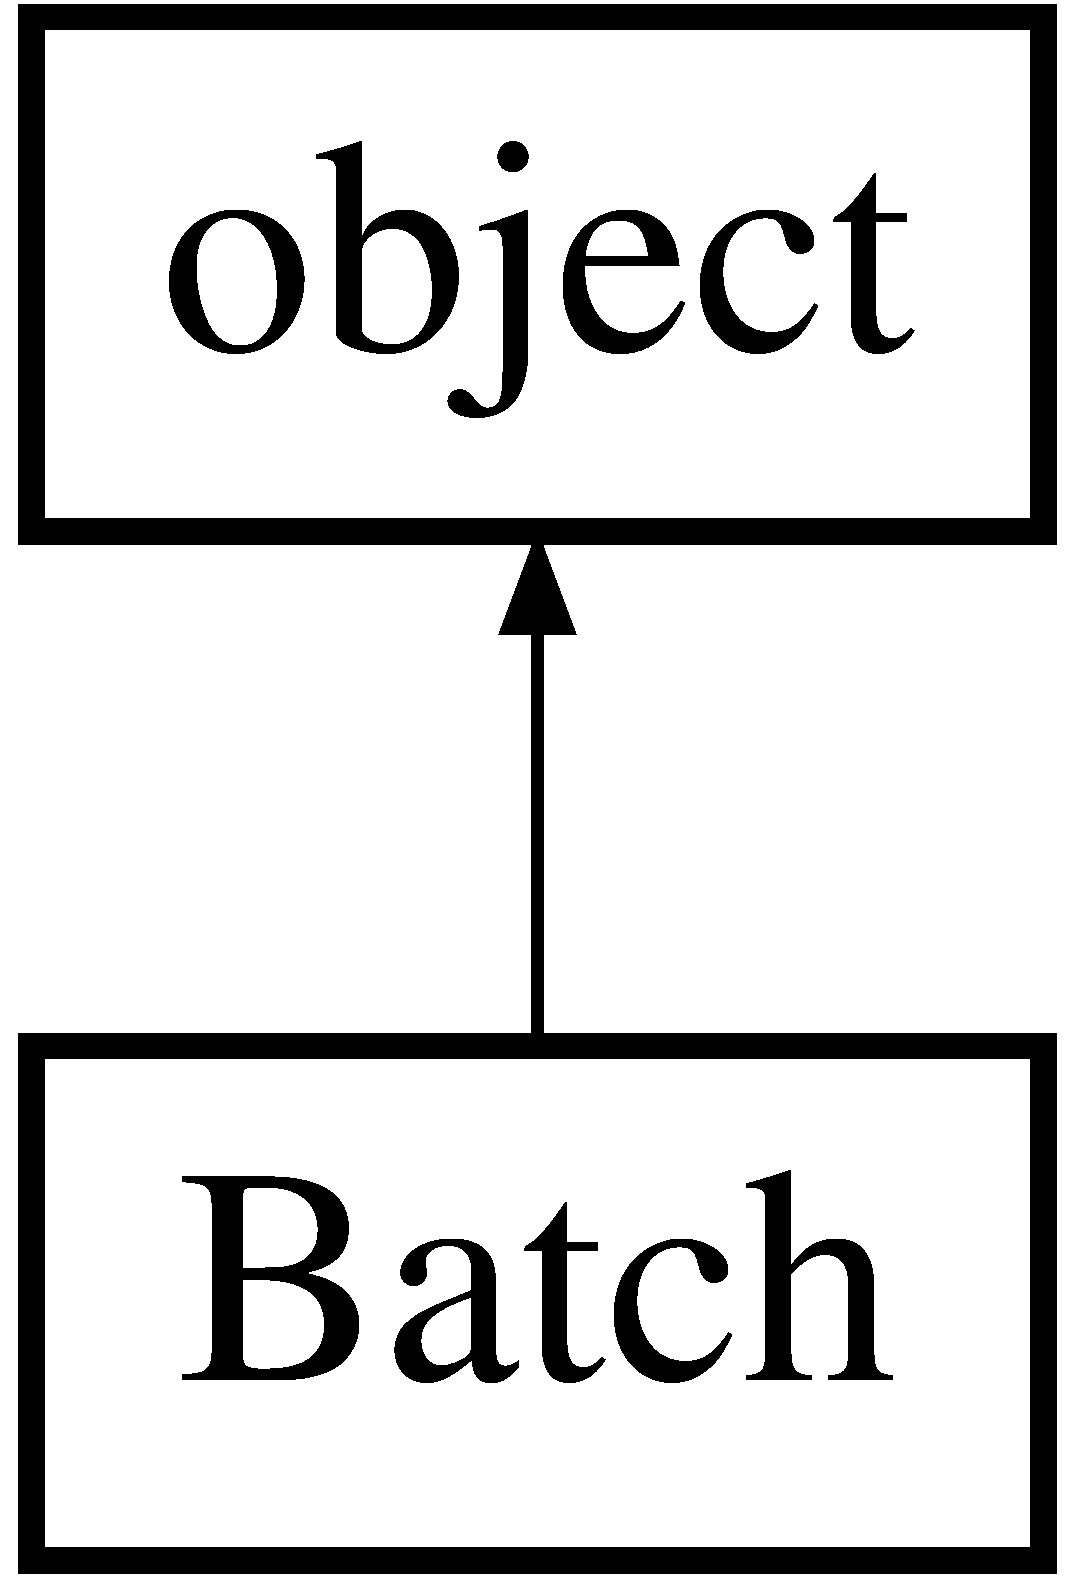
\includegraphics[height=2.000000cm]{classopenbu_1_1nax_1_1functions_1_1_batch}
\end{center}
\end{figure}
\doxysubsection*{Public Member Functions}
\doxysubsection*{Private Attributes}


The documentation for this class was generated from the following file\+:\begin{DoxyCompactItemize}
\item 
nax/functions.\+py\end{DoxyCompactItemize}

\hypertarget{classopenbu_1_1cell_1_1_cell}{}\doxysection{Cell Class Reference}
\label{classopenbu_1_1cell_1_1_cell}\index{Cell@{Cell}}
Inheritance diagram for Cell\+:\begin{figure}[H]
\begin{center}
\leavevmode
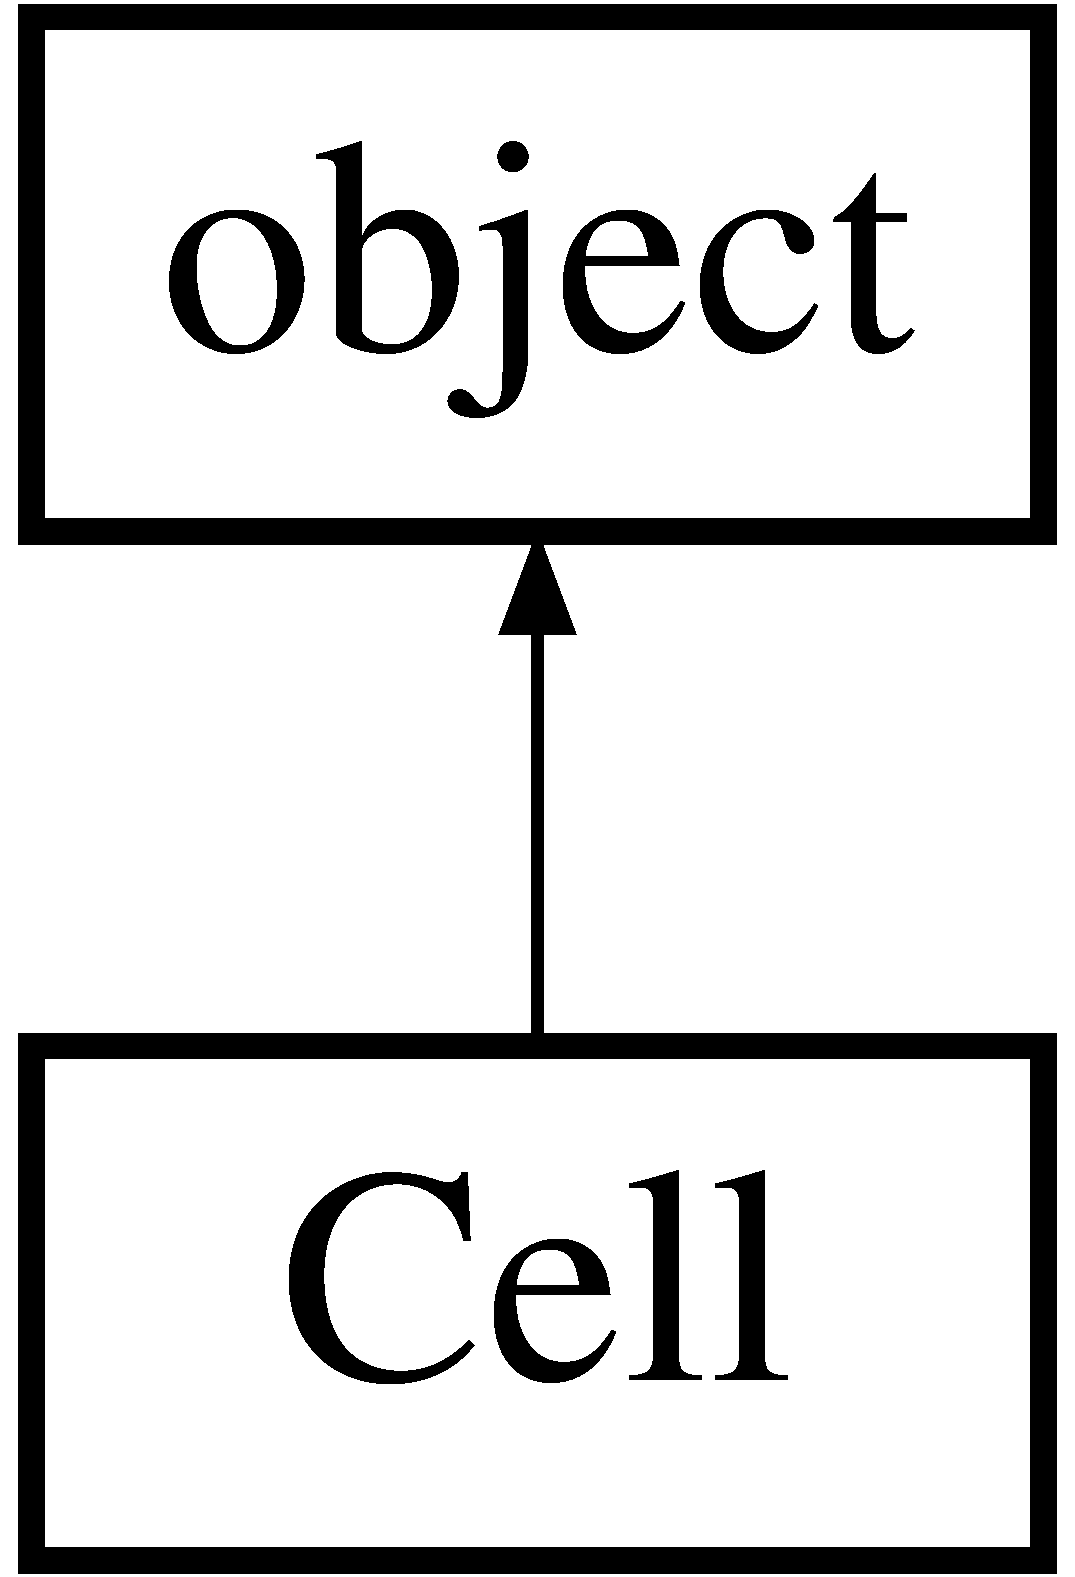
\includegraphics[height=2.000000cm]{classopenbu_1_1cell_1_1_cell}
\end{center}
\end{figure}
\doxysubsection*{Public Member Functions}
\doxysubsection*{Public Attributes}
\doxysubsection*{Static Public Attributes}
\doxysubsection*{Private Member Functions}
\doxysubsection*{Private Attributes}
\doxysubsection*{Static Private Attributes}


\doxysubsection{Member Function Documentation}
\mbox{\Hypertarget{classopenbu_1_1cell_1_1_cell_a60241928100db6ecdc4c8c3459506da9}\label{classopenbu_1_1cell_1_1_cell_a60241928100db6ecdc4c8c3459506da9}} 
\index{Cell@{Cell}!bu\_sec\_conv\_factor@{bu\_sec\_conv\_factor}}
\index{bu\_sec\_conv\_factor@{bu\_sec\_conv\_factor}!Cell@{Cell}}
\doxysubsubsection{\texorpdfstring{bu\_sec\_conv\_factor()}{bu\_sec\_conv\_factor()}}
{\footnotesize\ttfamily def bu\+\_\+sec\+\_\+conv\+\_\+factor (\begin{DoxyParamCaption}\item[{}]{self }\end{DoxyParamCaption})}

\begin{DoxyVerb}Returns the absolute values of the decay constant of the nuclide\end{DoxyVerb}
 \mbox{\Hypertarget{classopenbu_1_1cell_1_1_cell_a50ae19f4fbadad51e8a4d676c4d9866b}\label{classopenbu_1_1cell_1_1_cell_a50ae19f4fbadad51e8a4d676c4d9866b}} 
\index{Cell@{Cell}!ihm@{ihm}}
\index{ihm@{ihm}!Cell@{Cell}}
\doxysubsubsection{\texorpdfstring{ihm()}{ihm()}}
{\footnotesize\ttfamily def ihm (\begin{DoxyParamCaption}\item[{}]{self }\end{DoxyParamCaption})}

\begin{DoxyVerb}Returns the absolute values of the decay constant of the nuclide\end{DoxyVerb}
 

The documentation for this class was generated from the following file\+:\begin{DoxyCompactItemize}
\item 
cell.\+py\end{DoxyCompactItemize}

\hypertarget{classopenbu_1_1system_1_1_cell__name__not__found}{}\section{Cell\+\_\+name\+\_\+not\+\_\+found Class Reference}
\label{classopenbu_1_1system_1_1_cell__name__not__found}\index{Cell\+\_\+name\+\_\+not\+\_\+found@{Cell\+\_\+name\+\_\+not\+\_\+found}}
Inheritance diagram for Cell\+\_\+name\+\_\+not\+\_\+found\+:\begin{figure}[H]
\begin{center}
\leavevmode
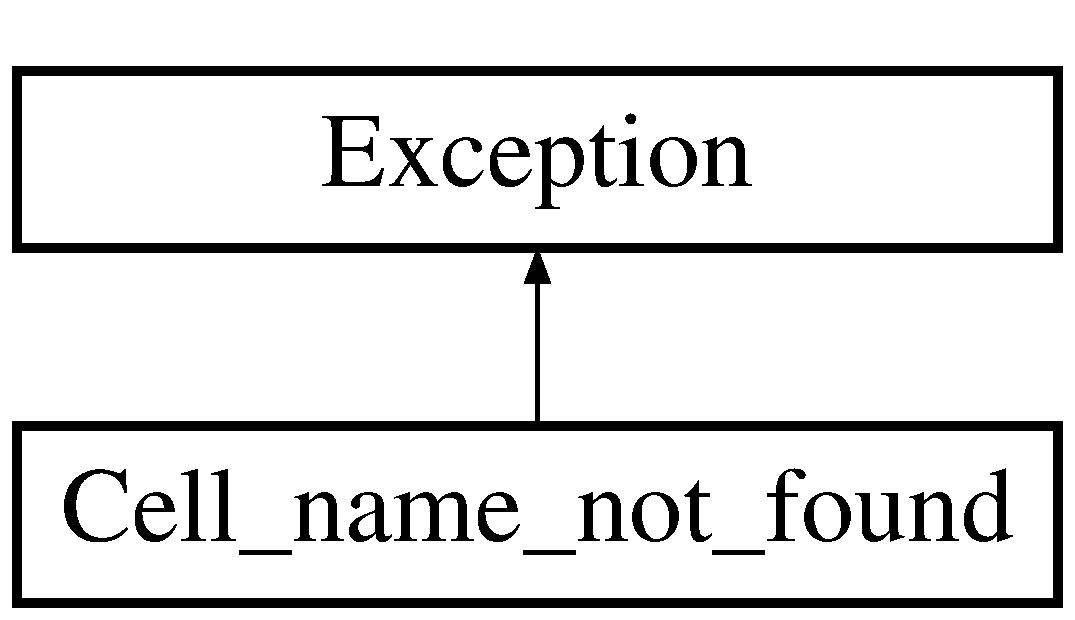
\includegraphics[height=2.000000cm]{classopenbu_1_1system_1_1_cell__name__not__found}
\end{center}
\end{figure}


The documentation for this class was generated from the following file\+:\begin{DoxyCompactItemize}
\item 
/\+Users/mouginot/work/app/\+Open\+B\+U/openbu/\mbox{\hyperlink{system_8py}{system.\+py}}\end{DoxyCompactItemize}

\hypertarget{classopenbu_1_1couple_1_1couple__openmc_1_1_couple__openmc}{}\section{Couple\+\_\+openmc Class Reference}
\label{classopenbu_1_1couple_1_1couple__openmc_1_1_couple__openmc}\index{Couple\+\_\+openmc@{Couple\+\_\+openmc}}
Inheritance diagram for Couple\+\_\+openmc\+:\begin{figure}[H]
\begin{center}
\leavevmode
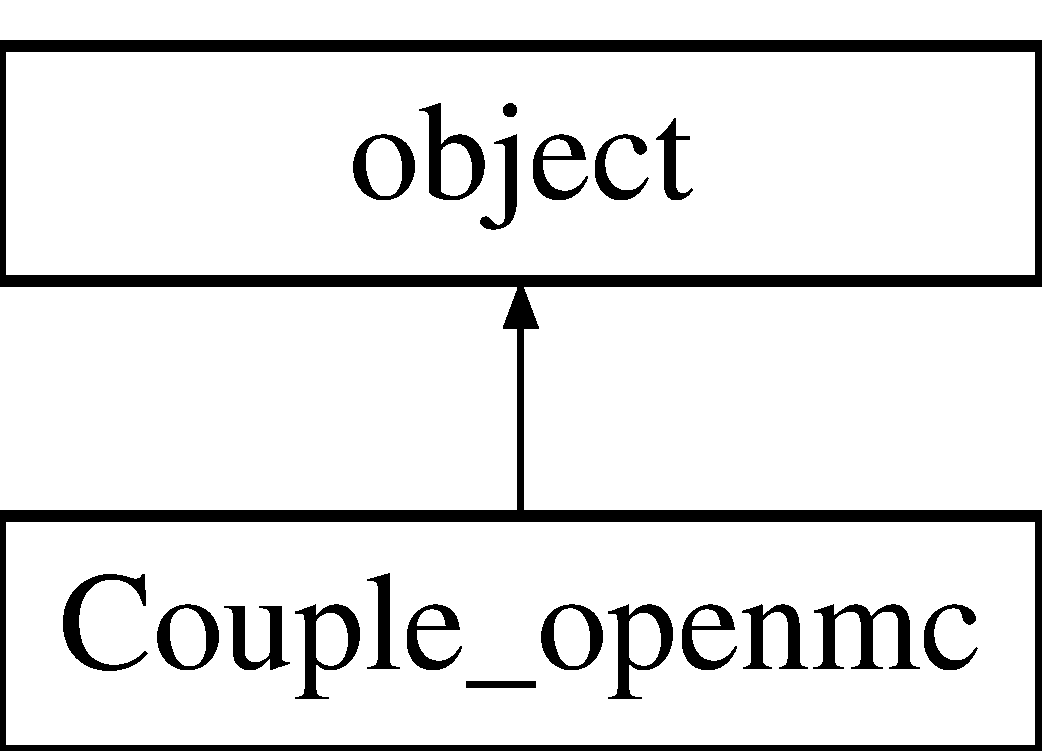
\includegraphics[height=2.000000cm]{classopenbu_1_1couple_1_1couple__openmc_1_1_couple__openmc}
\end{center}
\end{figure}
\subsection*{Public Member Functions}
\subsection*{Public Attributes}
\subsection*{Static Public Attributes}
\subsection*{Private Member Functions}
\subsection*{Private Attributes}


\subsection{Constructor \& Destructor Documentation}
\mbox{\Hypertarget{classopenbu_1_1couple_1_1couple__openmc_1_1_couple__openmc_adf43c036ad3b3850d41894aa20f4bd55}\label{classopenbu_1_1couple_1_1couple__openmc_1_1_couple__openmc_adf43c036ad3b3850d41894aa20f4bd55}} 
\index{openbu\+::couple\+::couple\+\_\+openmc\+::\+Couple\+\_\+openmc@{openbu\+::couple\+::couple\+\_\+openmc\+::\+Couple\+\_\+openmc}!\+\_\+\+\_\+init\+\_\+\+\_\+@{\+\_\+\+\_\+init\+\_\+\+\_\+}}
\index{\+\_\+\+\_\+init\+\_\+\+\_\+@{\+\_\+\+\_\+init\+\_\+\+\_\+}!openbu\+::couple\+::couple\+\_\+openmc\+::\+Couple\+\_\+openmc@{openbu\+::couple\+::couple\+\_\+openmc\+::\+Couple\+\_\+openmc}}
\subsubsection{\texorpdfstring{\+\_\+\+\_\+init\+\_\+\+\_\+()}{\_\_init\_\_()}}
{\footnotesize\ttfamily def \+\_\+\+\_\+init\+\_\+\+\_\+ (\begin{DoxyParamCaption}\item[{}]{self,  }\item[{}]{M\+C\+\_\+input\+\_\+path = {\ttfamily None},  }\item[{}]{xs\+\_\+mode = {\ttfamily \textquotesingle{}no~constant~lib\textquotesingle{}},  }\item[{}]{M\+PI = {\ttfamily None} }\end{DoxyParamCaption})}



\subsection{Member Function Documentation}
\mbox{\Hypertarget{classopenbu_1_1couple_1_1couple__openmc_1_1_couple__openmc_a2807161cebfc8c9d9811d8ee01fa2b7d}\label{classopenbu_1_1couple_1_1couple__openmc_1_1_couple__openmc_a2807161cebfc8c9d9811d8ee01fa2b7d}} 
\index{openbu\+::couple\+::couple\+\_\+openmc\+::\+Couple\+\_\+openmc@{openbu\+::couple\+::couple\+\_\+openmc\+::\+Couple\+\_\+openmc}!\+\_\+change\+\_\+cell\+\_\+materials@{\+\_\+change\+\_\+cell\+\_\+materials}}
\index{\+\_\+change\+\_\+cell\+\_\+materials@{\+\_\+change\+\_\+cell\+\_\+materials}!openbu\+::couple\+::couple\+\_\+openmc\+::\+Couple\+\_\+openmc@{openbu\+::couple\+::couple\+\_\+openmc\+::\+Couple\+\_\+openmc}}
\subsubsection{\texorpdfstring{\+\_\+change\+\_\+cell\+\_\+materials()}{\_change\_cell\_materials()}}
{\footnotesize\ttfamily def \+\_\+change\+\_\+cell\+\_\+materials (\begin{DoxyParamCaption}\item[{}]{self }\end{DoxyParamCaption})\hspace{0.3cm}{\ttfamily [private]}}

\mbox{\Hypertarget{classopenbu_1_1couple_1_1couple__openmc_1_1_couple__openmc_a3327925f8ff34893baf62d7d53f84ffb}\label{classopenbu_1_1couple_1_1couple__openmc_1_1_couple__openmc_a3327925f8ff34893baf62d7d53f84ffb}} 
\index{openbu\+::couple\+::couple\+\_\+openmc\+::\+Couple\+\_\+openmc@{openbu\+::couple\+::couple\+\_\+openmc\+::\+Couple\+\_\+openmc}!\+\_\+pre\+\_\+run@{\+\_\+pre\+\_\+run}}
\index{\+\_\+pre\+\_\+run@{\+\_\+pre\+\_\+run}!openbu\+::couple\+::couple\+\_\+openmc\+::\+Couple\+\_\+openmc@{openbu\+::couple\+::couple\+\_\+openmc\+::\+Couple\+\_\+openmc}}
\subsubsection{\texorpdfstring{\+\_\+pre\+\_\+run()}{\_pre\_run()}}
{\footnotesize\ttfamily def \+\_\+pre\+\_\+run (\begin{DoxyParamCaption}\item[{}]{self,  }\item[{}]{root\+\_\+cell }\end{DoxyParamCaption})\hspace{0.3cm}{\ttfamily [private]}}

\mbox{\Hypertarget{classopenbu_1_1couple_1_1couple__openmc_1_1_couple__openmc_acf4db72a2d51c96f541893afa86a3719}\label{classopenbu_1_1couple_1_1couple__openmc_1_1_couple__openmc_acf4db72a2d51c96f541893afa86a3719}} 
\index{openbu\+::couple\+::couple\+\_\+openmc\+::\+Couple\+\_\+openmc@{openbu\+::couple\+::couple\+\_\+openmc\+::\+Couple\+\_\+openmc}!\+\_\+read\+\_\+user\+\_\+settings@{\+\_\+read\+\_\+user\+\_\+settings}}
\index{\+\_\+read\+\_\+user\+\_\+settings@{\+\_\+read\+\_\+user\+\_\+settings}!openbu\+::couple\+::couple\+\_\+openmc\+::\+Couple\+\_\+openmc@{openbu\+::couple\+::couple\+\_\+openmc\+::\+Couple\+\_\+openmc}}
\subsubsection{\texorpdfstring{\+\_\+read\+\_\+user\+\_\+settings()}{\_read\_user\_settings()}}
{\footnotesize\ttfamily def \+\_\+read\+\_\+user\+\_\+settings (\begin{DoxyParamCaption}\item[{}]{self }\end{DoxyParamCaption})\hspace{0.3cm}{\ttfamily [private]}}

\mbox{\Hypertarget{classopenbu_1_1couple_1_1couple__openmc_1_1_couple__openmc_abb44be8f5b6e448c469f4751897dcba5}\label{classopenbu_1_1couple_1_1couple__openmc_1_1_couple__openmc_abb44be8f5b6e448c469f4751897dcba5}} 
\index{openbu\+::couple\+::couple\+\_\+openmc\+::\+Couple\+\_\+openmc@{openbu\+::couple\+::couple\+\_\+openmc\+::\+Couple\+\_\+openmc}!\+\_\+set\+\_\+cross\+\_\+sections\+\_\+path@{\+\_\+set\+\_\+cross\+\_\+sections\+\_\+path}}
\index{\+\_\+set\+\_\+cross\+\_\+sections\+\_\+path@{\+\_\+set\+\_\+cross\+\_\+sections\+\_\+path}!openbu\+::couple\+::couple\+\_\+openmc\+::\+Couple\+\_\+openmc@{openbu\+::couple\+::couple\+\_\+openmc\+::\+Couple\+\_\+openmc}}
\subsubsection{\texorpdfstring{\+\_\+set\+\_\+cross\+\_\+sections\+\_\+path()}{\_set\_cross\_sections\_path()}}
{\footnotesize\ttfamily def \+\_\+set\+\_\+cross\+\_\+sections\+\_\+path (\begin{DoxyParamCaption}\item[{}]{self,  }\item[{}]{pre\+\_\+run\+\_\+path }\end{DoxyParamCaption})\hspace{0.3cm}{\ttfamily [private]}}

\mbox{\Hypertarget{classopenbu_1_1couple_1_1couple__openmc_1_1_couple__openmc_a9f67057faef0b35164a7d17a24eebaff}\label{classopenbu_1_1couple_1_1couple__openmc_1_1_couple__openmc_a9f67057faef0b35164a7d17a24eebaff}} 
\index{openbu\+::couple\+::couple\+\_\+openmc\+::\+Couple\+\_\+openmc@{openbu\+::couple\+::couple\+\_\+openmc\+::\+Couple\+\_\+openmc}!\+\_\+set\+\_\+initial\+\_\+summary@{\+\_\+set\+\_\+initial\+\_\+summary}}
\index{\+\_\+set\+\_\+initial\+\_\+summary@{\+\_\+set\+\_\+initial\+\_\+summary}!openbu\+::couple\+::couple\+\_\+openmc\+::\+Couple\+\_\+openmc@{openbu\+::couple\+::couple\+\_\+openmc\+::\+Couple\+\_\+openmc}}
\subsubsection{\texorpdfstring{\+\_\+set\+\_\+initial\+\_\+summary()}{\_set\_initial\_summary()}}
{\footnotesize\ttfamily def \+\_\+set\+\_\+initial\+\_\+summary (\begin{DoxyParamCaption}\item[{}]{self,  }\item[{}]{path = {\ttfamily os.getcwd()} }\end{DoxyParamCaption})\hspace{0.3cm}{\ttfamily [private]}}

\mbox{\Hypertarget{classopenbu_1_1couple_1_1couple__openmc_1_1_couple__openmc_aa59058755f41ba2b0de1b748356e480d}\label{classopenbu_1_1couple_1_1couple__openmc_1_1_couple__openmc_aa59058755f41ba2b0de1b748356e480d}} 
\index{openbu\+::couple\+::couple\+\_\+openmc\+::\+Couple\+\_\+openmc@{openbu\+::couple\+::couple\+\_\+openmc\+::\+Couple\+\_\+openmc}!\+\_\+set\+\_\+kinf@{\+\_\+set\+\_\+kinf}}
\index{\+\_\+set\+\_\+kinf@{\+\_\+set\+\_\+kinf}!openbu\+::couple\+::couple\+\_\+openmc\+::\+Couple\+\_\+openmc@{openbu\+::couple\+::couple\+\_\+openmc\+::\+Couple\+\_\+openmc}}
\subsubsection{\texorpdfstring{\+\_\+set\+\_\+kinf()}{\_set\_kinf()}}
{\footnotesize\ttfamily def \+\_\+set\+\_\+kinf (\begin{DoxyParamCaption}\item[{}]{self }\end{DoxyParamCaption})\hspace{0.3cm}{\ttfamily [private]}}

\mbox{\Hypertarget{classopenbu_1_1couple_1_1couple__openmc_1_1_couple__openmc_a484f34b7e4eceac67c32eff27a97d39e}\label{classopenbu_1_1couple_1_1couple__openmc_1_1_couple__openmc_a484f34b7e4eceac67c32eff27a97d39e}} 
\index{openbu\+::couple\+::couple\+\_\+openmc\+::\+Couple\+\_\+openmc@{openbu\+::couple\+::couple\+\_\+openmc\+::\+Couple\+\_\+openmc}!\+\_\+set\+\_\+root\+\_\+cell@{\+\_\+set\+\_\+root\+\_\+cell}}
\index{\+\_\+set\+\_\+root\+\_\+cell@{\+\_\+set\+\_\+root\+\_\+cell}!openbu\+::couple\+::couple\+\_\+openmc\+::\+Couple\+\_\+openmc@{openbu\+::couple\+::couple\+\_\+openmc\+::\+Couple\+\_\+openmc}}
\subsubsection{\texorpdfstring{\+\_\+set\+\_\+root\+\_\+cell()}{\_set\_root\_cell()}}
{\footnotesize\ttfamily def \+\_\+set\+\_\+root\+\_\+cell (\begin{DoxyParamCaption}\item[{}]{self,  }\item[{}]{root\+\_\+cell\+\_\+name }\end{DoxyParamCaption})\hspace{0.3cm}{\ttfamily [private]}}

\mbox{\Hypertarget{classopenbu_1_1couple_1_1couple__openmc_1_1_couple__openmc_ae9625e393903a346dc9d684fdf192edb}\label{classopenbu_1_1couple_1_1couple__openmc_1_1_couple__openmc_ae9625e393903a346dc9d684fdf192edb}} 
\index{openbu\+::couple\+::couple\+\_\+openmc\+::\+Couple\+\_\+openmc@{openbu\+::couple\+::couple\+\_\+openmc\+::\+Couple\+\_\+openmc}!\+\_\+set\+\_\+statepoint@{\+\_\+set\+\_\+statepoint}}
\index{\+\_\+set\+\_\+statepoint@{\+\_\+set\+\_\+statepoint}!openbu\+::couple\+::couple\+\_\+openmc\+::\+Couple\+\_\+openmc@{openbu\+::couple\+::couple\+\_\+openmc\+::\+Couple\+\_\+openmc}}
\subsubsection{\texorpdfstring{\+\_\+set\+\_\+statepoint()}{\_set\_statepoint()}}
{\footnotesize\ttfamily def \+\_\+set\+\_\+statepoint (\begin{DoxyParamCaption}\item[{}]{self,  }\item[{}]{path = {\ttfamily os.getcwd()} }\end{DoxyParamCaption})\hspace{0.3cm}{\ttfamily [private]}}

\mbox{\Hypertarget{classopenbu_1_1couple_1_1couple__openmc_1_1_couple__openmc_a4956616a2a93a4106d31b765439b9ab7}\label{classopenbu_1_1couple_1_1couple__openmc_1_1_couple__openmc_a4956616a2a93a4106d31b765439b9ab7}} 
\index{openbu\+::couple\+::couple\+\_\+openmc\+::\+Couple\+\_\+openmc@{openbu\+::couple\+::couple\+\_\+openmc\+::\+Couple\+\_\+openmc}!\+\_\+set\+\_\+updated\+\_\+summary@{\+\_\+set\+\_\+updated\+\_\+summary}}
\index{\+\_\+set\+\_\+updated\+\_\+summary@{\+\_\+set\+\_\+updated\+\_\+summary}!openbu\+::couple\+::couple\+\_\+openmc\+::\+Couple\+\_\+openmc@{openbu\+::couple\+::couple\+\_\+openmc\+::\+Couple\+\_\+openmc}}
\subsubsection{\texorpdfstring{\+\_\+set\+\_\+updated\+\_\+summary()}{\_set\_updated\_summary()}}
{\footnotesize\ttfamily def \+\_\+set\+\_\+updated\+\_\+summary (\begin{DoxyParamCaption}\item[{}]{self,  }\item[{}]{path = {\ttfamily os.getcwd()} }\end{DoxyParamCaption})\hspace{0.3cm}{\ttfamily [private]}}

\mbox{\Hypertarget{classopenbu_1_1couple_1_1couple__openmc_1_1_couple__openmc_ac6a7964c7f1c353377b2c4dadc5f50a1}\label{classopenbu_1_1couple_1_1couple__openmc_1_1_couple__openmc_ac6a7964c7f1c353377b2c4dadc5f50a1}} 
\index{openbu\+::couple\+::couple\+\_\+openmc\+::\+Couple\+\_\+openmc@{openbu\+::couple\+::couple\+\_\+openmc\+::\+Couple\+\_\+openmc}!add\+\_\+zero\+\_\+dens\+\_\+nuclides@{add\+\_\+zero\+\_\+dens\+\_\+nuclides}}
\index{add\+\_\+zero\+\_\+dens\+\_\+nuclides@{add\+\_\+zero\+\_\+dens\+\_\+nuclides}!openbu\+::couple\+::couple\+\_\+openmc\+::\+Couple\+\_\+openmc@{openbu\+::couple\+::couple\+\_\+openmc\+::\+Couple\+\_\+openmc}}
\subsubsection{\texorpdfstring{add\+\_\+zero\+\_\+dens\+\_\+nuclides()}{add\_zero\_dens\_nuclides()}}
{\footnotesize\ttfamily def add\+\_\+zero\+\_\+dens\+\_\+nuclides (\begin{DoxyParamCaption}\item[{}]{self,  }\item[{}]{cell }\end{DoxyParamCaption})}

\mbox{\Hypertarget{classopenbu_1_1couple_1_1couple__openmc_1_1_couple__openmc_aee8e543a1329dd01ede1e96434b89412}\label{classopenbu_1_1couple_1_1couple__openmc_1_1_couple__openmc_aee8e543a1329dd01ede1e96434b89412}} 
\index{openbu\+::couple\+::couple\+\_\+openmc\+::\+Couple\+\_\+openmc@{openbu\+::couple\+::couple\+\_\+openmc\+::\+Couple\+\_\+openmc}!batches@{batches}}
\index{batches@{batches}!openbu\+::couple\+::couple\+\_\+openmc\+::\+Couple\+\_\+openmc@{openbu\+::couple\+::couple\+\_\+openmc\+::\+Couple\+\_\+openmc}}
\subsubsection{\texorpdfstring{batches()}{batches()}\hspace{0.1cm}{\footnotesize\ttfamily [1/2]}}
{\footnotesize\ttfamily def batches (\begin{DoxyParamCaption}\item[{}]{self }\end{DoxyParamCaption})}

\mbox{\Hypertarget{classopenbu_1_1couple_1_1couple__openmc_1_1_couple__openmc_ab44c2a368eef406c7d2c712a57bbc807}\label{classopenbu_1_1couple_1_1couple__openmc_1_1_couple__openmc_ab44c2a368eef406c7d2c712a57bbc807}} 
\index{openbu\+::couple\+::couple\+\_\+openmc\+::\+Couple\+\_\+openmc@{openbu\+::couple\+::couple\+\_\+openmc\+::\+Couple\+\_\+openmc}!batches@{batches}}
\index{batches@{batches}!openbu\+::couple\+::couple\+\_\+openmc\+::\+Couple\+\_\+openmc@{openbu\+::couple\+::couple\+\_\+openmc\+::\+Couple\+\_\+openmc}}
\subsubsection{\texorpdfstring{batches()}{batches()}\hspace{0.1cm}{\footnotesize\ttfamily [2/2]}}
{\footnotesize\ttfamily def batches (\begin{DoxyParamCaption}\item[{}]{self,  }\item[{}]{batches }\end{DoxyParamCaption})}

\mbox{\Hypertarget{classopenbu_1_1couple_1_1couple__openmc_1_1_couple__openmc_aa488db59629eb4dccde6e0c71edeb2d4}\label{classopenbu_1_1couple_1_1couple__openmc_1_1_couple__openmc_aa488db59629eb4dccde6e0c71edeb2d4}} 
\index{openbu\+::couple\+::couple\+\_\+openmc\+::\+Couple\+\_\+openmc@{openbu\+::couple\+::couple\+\_\+openmc\+::\+Couple\+\_\+openmc}!bounding\+\_\+box@{bounding\+\_\+box}}
\index{bounding\+\_\+box@{bounding\+\_\+box}!openbu\+::couple\+::couple\+\_\+openmc\+::\+Couple\+\_\+openmc@{openbu\+::couple\+::couple\+\_\+openmc\+::\+Couple\+\_\+openmc}}
\subsubsection{\texorpdfstring{bounding\+\_\+box()}{bounding\_box()}}
{\footnotesize\ttfamily def bounding\+\_\+box (\begin{DoxyParamCaption}\item[{}]{self }\end{DoxyParamCaption})}

\mbox{\Hypertarget{classopenbu_1_1couple_1_1couple__openmc_1_1_couple__openmc_a5968b12da4d1097f8c5309aaf43ad278}\label{classopenbu_1_1couple_1_1couple__openmc_1_1_couple__openmc_a5968b12da4d1097f8c5309aaf43ad278}} 
\index{openbu\+::couple\+::couple\+\_\+openmc\+::\+Couple\+\_\+openmc@{openbu\+::couple\+::couple\+\_\+openmc\+::\+Couple\+\_\+openmc}!burn@{burn}}
\index{burn@{burn}!openbu\+::couple\+::couple\+\_\+openmc\+::\+Couple\+\_\+openmc@{openbu\+::couple\+::couple\+\_\+openmc\+::\+Couple\+\_\+openmc}}
\subsubsection{\texorpdfstring{burn()}{burn()}}
{\footnotesize\ttfamily def burn (\begin{DoxyParamCaption}\item[{}]{self }\end{DoxyParamCaption})}

\mbox{\Hypertarget{classopenbu_1_1couple_1_1couple__openmc_1_1_couple__openmc_adc4ee3a13db3358ffdd3d69492377e74}\label{classopenbu_1_1couple_1_1couple__openmc_1_1_couple__openmc_adc4ee3a13db3358ffdd3d69492377e74}} 
\index{openbu\+::couple\+::couple\+\_\+openmc\+::\+Couple\+\_\+openmc@{openbu\+::couple\+::couple\+\_\+openmc\+::\+Couple\+\_\+openmc}!copy\+\_\+\+M\+C\+\_\+files@{copy\+\_\+\+M\+C\+\_\+files}}
\index{copy\+\_\+\+M\+C\+\_\+files@{copy\+\_\+\+M\+C\+\_\+files}!openbu\+::couple\+::couple\+\_\+openmc\+::\+Couple\+\_\+openmc@{openbu\+::couple\+::couple\+\_\+openmc\+::\+Couple\+\_\+openmc}}
\subsubsection{\texorpdfstring{copy\+\_\+\+M\+C\+\_\+files()}{copy\_MC\_files()}}
{\footnotesize\ttfamily def copy\+\_\+\+M\+C\+\_\+files (\begin{DoxyParamCaption}\item[{}]{self,  }\item[{}]{s }\end{DoxyParamCaption})}

\mbox{\Hypertarget{classopenbu_1_1couple_1_1couple__openmc_1_1_couple__openmc_a1b61b8a8e7322d2b0a30da7d5c9c971b}\label{classopenbu_1_1couple_1_1couple__openmc_1_1_couple__openmc_a1b61b8a8e7322d2b0a30da7d5c9c971b}} 
\index{openbu\+::couple\+::couple\+\_\+openmc\+::\+Couple\+\_\+openmc@{openbu\+::couple\+::couple\+\_\+openmc\+::\+Couple\+\_\+openmc}!copy\+\_\+user\+\_\+input@{copy\+\_\+user\+\_\+input}}
\index{copy\+\_\+user\+\_\+input@{copy\+\_\+user\+\_\+input}!openbu\+::couple\+::couple\+\_\+openmc\+::\+Couple\+\_\+openmc@{openbu\+::couple\+::couple\+\_\+openmc\+::\+Couple\+\_\+openmc}}
\subsubsection{\texorpdfstring{copy\+\_\+user\+\_\+input()}{copy\_user\_input()}}
{\footnotesize\ttfamily def copy\+\_\+user\+\_\+input (\begin{DoxyParamCaption}\item[{}]{self }\end{DoxyParamCaption})}

\mbox{\Hypertarget{classopenbu_1_1couple_1_1couple__openmc_1_1_couple__openmc_a828e2a249e1882bf8cddb58796cfe16d}\label{classopenbu_1_1couple_1_1couple__openmc_1_1_couple__openmc_a828e2a249e1882bf8cddb58796cfe16d}} 
\index{openbu\+::couple\+::couple\+\_\+openmc\+::\+Couple\+\_\+openmc@{openbu\+::couple\+::couple\+\_\+openmc\+::\+Couple\+\_\+openmc}!export\+\_\+geometry\+\_\+to\+\_\+xml@{export\+\_\+geometry\+\_\+to\+\_\+xml}}
\index{export\+\_\+geometry\+\_\+to\+\_\+xml@{export\+\_\+geometry\+\_\+to\+\_\+xml}!openbu\+::couple\+::couple\+\_\+openmc\+::\+Couple\+\_\+openmc@{openbu\+::couple\+::couple\+\_\+openmc\+::\+Couple\+\_\+openmc}}
\subsubsection{\texorpdfstring{export\+\_\+geometry\+\_\+to\+\_\+xml()}{export\_geometry\_to\_xml()}}
{\footnotesize\ttfamily def export\+\_\+geometry\+\_\+to\+\_\+xml (\begin{DoxyParamCaption}\item[{}]{self }\end{DoxyParamCaption})}

\mbox{\Hypertarget{classopenbu_1_1couple_1_1couple__openmc_1_1_couple__openmc_ab0f5e73d13112cb5e1d16c32add9c698}\label{classopenbu_1_1couple_1_1couple__openmc_1_1_couple__openmc_ab0f5e73d13112cb5e1d16c32add9c698}} 
\index{openbu\+::couple\+::couple\+\_\+openmc\+::\+Couple\+\_\+openmc@{openbu\+::couple\+::couple\+\_\+openmc\+::\+Couple\+\_\+openmc}!export\+\_\+material\+\_\+to\+\_\+xml@{export\+\_\+material\+\_\+to\+\_\+xml}}
\index{export\+\_\+material\+\_\+to\+\_\+xml@{export\+\_\+material\+\_\+to\+\_\+xml}!openbu\+::couple\+::couple\+\_\+openmc\+::\+Couple\+\_\+openmc@{openbu\+::couple\+::couple\+\_\+openmc\+::\+Couple\+\_\+openmc}}
\subsubsection{\texorpdfstring{export\+\_\+material\+\_\+to\+\_\+xml()}{export\_material\_to\_xml()}}
{\footnotesize\ttfamily def export\+\_\+material\+\_\+to\+\_\+xml (\begin{DoxyParamCaption}\item[{}]{self }\end{DoxyParamCaption})}

\mbox{\Hypertarget{classopenbu_1_1couple_1_1couple__openmc_1_1_couple__openmc_a947e7cc8a90a2a4efa9944c84e5f0323}\label{classopenbu_1_1couple_1_1couple__openmc_1_1_couple__openmc_a947e7cc8a90a2a4efa9944c84e5f0323}} 
\index{openbu\+::couple\+::couple\+\_\+openmc\+::\+Couple\+\_\+openmc@{openbu\+::couple\+::couple\+\_\+openmc\+::\+Couple\+\_\+openmc}!export\+\_\+settings\+\_\+to\+\_\+xml@{export\+\_\+settings\+\_\+to\+\_\+xml}}
\index{export\+\_\+settings\+\_\+to\+\_\+xml@{export\+\_\+settings\+\_\+to\+\_\+xml}!openbu\+::couple\+::couple\+\_\+openmc\+::\+Couple\+\_\+openmc@{openbu\+::couple\+::couple\+\_\+openmc\+::\+Couple\+\_\+openmc}}
\subsubsection{\texorpdfstring{export\+\_\+settings\+\_\+to\+\_\+xml()}{export\_settings\_to\_xml()}}
{\footnotesize\ttfamily def export\+\_\+settings\+\_\+to\+\_\+xml (\begin{DoxyParamCaption}\item[{}]{self }\end{DoxyParamCaption})}

\mbox{\Hypertarget{classopenbu_1_1couple_1_1couple__openmc_1_1_couple__openmc_ab93dec4678af3338259e4abe79b31c6d}\label{classopenbu_1_1couple_1_1couple__openmc_1_1_couple__openmc_ab93dec4678af3338259e4abe79b31c6d}} 
\index{openbu\+::couple\+::couple\+\_\+openmc\+::\+Couple\+\_\+openmc@{openbu\+::couple\+::couple\+\_\+openmc\+::\+Couple\+\_\+openmc}!export\+\_\+tallies\+\_\+to\+\_\+xml@{export\+\_\+tallies\+\_\+to\+\_\+xml}}
\index{export\+\_\+tallies\+\_\+to\+\_\+xml@{export\+\_\+tallies\+\_\+to\+\_\+xml}!openbu\+::couple\+::couple\+\_\+openmc\+::\+Couple\+\_\+openmc@{openbu\+::couple\+::couple\+\_\+openmc\+::\+Couple\+\_\+openmc}}
\subsubsection{\texorpdfstring{export\+\_\+tallies\+\_\+to\+\_\+xml()}{export\_tallies\_to\_xml()}}
{\footnotesize\ttfamily def export\+\_\+tallies\+\_\+to\+\_\+xml (\begin{DoxyParamCaption}\item[{}]{self }\end{DoxyParamCaption})}

\mbox{\Hypertarget{classopenbu_1_1couple_1_1couple__openmc_1_1_couple__openmc_a3171ea6d58bef26700680e0fa2f2643c}\label{classopenbu_1_1couple_1_1couple__openmc_1_1_couple__openmc_a3171ea6d58bef26700680e0fa2f2643c}} 
\index{openbu\+::couple\+::couple\+\_\+openmc\+::\+Couple\+\_\+openmc@{openbu\+::couple\+::couple\+\_\+openmc\+::\+Couple\+\_\+openmc}!gen\+\_\+user\+\_\+input\+\_\+folder@{gen\+\_\+user\+\_\+input\+\_\+folder}}
\index{gen\+\_\+user\+\_\+input\+\_\+folder@{gen\+\_\+user\+\_\+input\+\_\+folder}!openbu\+::couple\+::couple\+\_\+openmc\+::\+Couple\+\_\+openmc@{openbu\+::couple\+::couple\+\_\+openmc\+::\+Couple\+\_\+openmc}}
\subsubsection{\texorpdfstring{gen\+\_\+user\+\_\+input\+\_\+folder()}{gen\_user\_input\_folder()}}
{\footnotesize\ttfamily def gen\+\_\+user\+\_\+input\+\_\+folder (\begin{DoxyParamCaption}\item[{}]{self }\end{DoxyParamCaption})}

\mbox{\Hypertarget{classopenbu_1_1couple_1_1couple__openmc_1_1_couple__openmc_ac271eb1deae1f744a01e8b1a057369d5}\label{classopenbu_1_1couple_1_1couple__openmc_1_1_couple__openmc_ac271eb1deae1f744a01e8b1a057369d5}} 
\index{openbu\+::couple\+::couple\+\_\+openmc\+::\+Couple\+\_\+openmc@{openbu\+::couple\+::couple\+\_\+openmc\+::\+Couple\+\_\+openmc}!get\+\_\+all\+\_\+nucl\+\_\+rxn\+\_\+tally@{get\+\_\+all\+\_\+nucl\+\_\+rxn\+\_\+tally}}
\index{get\+\_\+all\+\_\+nucl\+\_\+rxn\+\_\+tally@{get\+\_\+all\+\_\+nucl\+\_\+rxn\+\_\+tally}!openbu\+::couple\+::couple\+\_\+openmc\+::\+Couple\+\_\+openmc@{openbu\+::couple\+::couple\+\_\+openmc\+::\+Couple\+\_\+openmc}}
\subsubsection{\texorpdfstring{get\+\_\+all\+\_\+nucl\+\_\+rxn\+\_\+tally()}{get\_all\_nucl\_rxn\_tally()}}
{\footnotesize\ttfamily def get\+\_\+all\+\_\+nucl\+\_\+rxn\+\_\+tally (\begin{DoxyParamCaption}\item[{}]{self,  }\item[{}]{bucell }\end{DoxyParamCaption})}

\mbox{\Hypertarget{classopenbu_1_1couple_1_1couple__openmc_1_1_couple__openmc_ac3455eb5524078caf131880d2acb90da}\label{classopenbu_1_1couple_1_1couple__openmc_1_1_couple__openmc_ac3455eb5524078caf131880d2acb90da}} 
\index{openbu\+::couple\+::couple\+\_\+openmc\+::\+Couple\+\_\+openmc@{openbu\+::couple\+::couple\+\_\+openmc\+::\+Couple\+\_\+openmc}!get\+\_\+bucell\+\_\+from\+\_\+cell@{get\+\_\+bucell\+\_\+from\+\_\+cell}}
\index{get\+\_\+bucell\+\_\+from\+\_\+cell@{get\+\_\+bucell\+\_\+from\+\_\+cell}!openbu\+::couple\+::couple\+\_\+openmc\+::\+Couple\+\_\+openmc@{openbu\+::couple\+::couple\+\_\+openmc\+::\+Couple\+\_\+openmc}}
\subsubsection{\texorpdfstring{get\+\_\+bucell\+\_\+from\+\_\+cell()}{get\_bucell\_from\_cell()}}
{\footnotesize\ttfamily def get\+\_\+bucell\+\_\+from\+\_\+cell (\begin{DoxyParamCaption}\item[{}]{self }\end{DoxyParamCaption})}

\mbox{\Hypertarget{classopenbu_1_1couple_1_1couple__openmc_1_1_couple__openmc_ad4720dcbea2a2ee736df2befd86ae244}\label{classopenbu_1_1couple_1_1couple__openmc_1_1_couple__openmc_ad4720dcbea2a2ee736df2befd86ae244}} 
\index{openbu\+::couple\+::couple\+\_\+openmc\+::\+Couple\+\_\+openmc@{openbu\+::couple\+::couple\+\_\+openmc\+::\+Couple\+\_\+openmc}!get\+\_\+flux\+\_\+spectrum\+\_\+tally@{get\+\_\+flux\+\_\+spectrum\+\_\+tally}}
\index{get\+\_\+flux\+\_\+spectrum\+\_\+tally@{get\+\_\+flux\+\_\+spectrum\+\_\+tally}!openbu\+::couple\+::couple\+\_\+openmc\+::\+Couple\+\_\+openmc@{openbu\+::couple\+::couple\+\_\+openmc\+::\+Couple\+\_\+openmc}}
\subsubsection{\texorpdfstring{get\+\_\+flux\+\_\+spectrum\+\_\+tally()}{get\_flux\_spectrum\_tally()}}
{\footnotesize\ttfamily def get\+\_\+flux\+\_\+spectrum\+\_\+tally (\begin{DoxyParamCaption}\item[{}]{self,  }\item[{}]{bucell }\end{DoxyParamCaption})}

\mbox{\Hypertarget{classopenbu_1_1couple_1_1couple__openmc_1_1_couple__openmc_a1aced28963235c39892bfb7eb025dd74}\label{classopenbu_1_1couple_1_1couple__openmc_1_1_couple__openmc_a1aced28963235c39892bfb7eb025dd74}} 
\index{openbu\+::couple\+::couple\+\_\+openmc\+::\+Couple\+\_\+openmc@{openbu\+::couple\+::couple\+\_\+openmc\+::\+Couple\+\_\+openmc}!get\+\_\+flux\+\_\+tally@{get\+\_\+flux\+\_\+tally}}
\index{get\+\_\+flux\+\_\+tally@{get\+\_\+flux\+\_\+tally}!openbu\+::couple\+::couple\+\_\+openmc\+::\+Couple\+\_\+openmc@{openbu\+::couple\+::couple\+\_\+openmc\+::\+Couple\+\_\+openmc}}
\subsubsection{\texorpdfstring{get\+\_\+flux\+\_\+tally()}{get\_flux\_tally()}}
{\footnotesize\ttfamily def get\+\_\+flux\+\_\+tally (\begin{DoxyParamCaption}\item[{}]{self,  }\item[{}]{bucell }\end{DoxyParamCaption})}

\mbox{\Hypertarget{classopenbu_1_1couple_1_1couple__openmc_1_1_couple__openmc_a27a2ccd2322a747e248cb8c953b20d13}\label{classopenbu_1_1couple_1_1couple__openmc_1_1_couple__openmc_a27a2ccd2322a747e248cb8c953b20d13}} 
\index{openbu\+::couple\+::couple\+\_\+openmc\+::\+Couple\+\_\+openmc@{openbu\+::couple\+::couple\+\_\+openmc\+::\+Couple\+\_\+openmc}!get\+\_\+nucl\+\_\+to\+\_\+be\+\_\+tallied@{get\+\_\+nucl\+\_\+to\+\_\+be\+\_\+tallied}}
\index{get\+\_\+nucl\+\_\+to\+\_\+be\+\_\+tallied@{get\+\_\+nucl\+\_\+to\+\_\+be\+\_\+tallied}!openbu\+::couple\+::couple\+\_\+openmc\+::\+Couple\+\_\+openmc@{openbu\+::couple\+::couple\+\_\+openmc\+::\+Couple\+\_\+openmc}}
\subsubsection{\texorpdfstring{get\+\_\+nucl\+\_\+to\+\_\+be\+\_\+tallied()}{get\_nucl\_to\_be\_tallied()}}
{\footnotesize\ttfamily def get\+\_\+nucl\+\_\+to\+\_\+be\+\_\+tallied (\begin{DoxyParamCaption}\item[{}]{self,  }\item[{}]{bucell }\end{DoxyParamCaption})}

\mbox{\Hypertarget{classopenbu_1_1couple_1_1couple__openmc_1_1_couple__openmc_a6aa7288e7a8ac6a95fa650bfc866c0b0}\label{classopenbu_1_1couple_1_1couple__openmc_1_1_couple__openmc_a6aa7288e7a8ac6a95fa650bfc866c0b0}} 
\index{openbu\+::couple\+::couple\+\_\+openmc\+::\+Couple\+\_\+openmc@{openbu\+::couple\+::couple\+\_\+openmc\+::\+Couple\+\_\+openmc}!import\+\_\+openmc@{import\+\_\+openmc}}
\index{import\+\_\+openmc@{import\+\_\+openmc}!openbu\+::couple\+::couple\+\_\+openmc\+::\+Couple\+\_\+openmc@{openbu\+::couple\+::couple\+\_\+openmc\+::\+Couple\+\_\+openmc}}
\subsubsection{\texorpdfstring{import\+\_\+openmc()}{import\_openmc()}}
{\footnotesize\ttfamily def import\+\_\+openmc (\begin{DoxyParamCaption}\item[{}]{self,  }\item[{}]{root\+\_\+cell }\end{DoxyParamCaption})}

\mbox{\Hypertarget{classopenbu_1_1couple_1_1couple__openmc_1_1_couple__openmc_ac27a2578faf8d6c48276ebfd5713d434}\label{classopenbu_1_1couple_1_1couple__openmc_1_1_couple__openmc_ac27a2578faf8d6c48276ebfd5713d434}} 
\index{openbu\+::couple\+::couple\+\_\+openmc\+::\+Couple\+\_\+openmc@{openbu\+::couple\+::couple\+\_\+openmc\+::\+Couple\+\_\+openmc}!inactive@{inactive}}
\index{inactive@{inactive}!openbu\+::couple\+::couple\+\_\+openmc\+::\+Couple\+\_\+openmc@{openbu\+::couple\+::couple\+\_\+openmc\+::\+Couple\+\_\+openmc}}
\subsubsection{\texorpdfstring{inactive()}{inactive()}\hspace{0.1cm}{\footnotesize\ttfamily [1/2]}}
{\footnotesize\ttfamily def inactive (\begin{DoxyParamCaption}\item[{}]{self }\end{DoxyParamCaption})}

\mbox{\Hypertarget{classopenbu_1_1couple_1_1couple__openmc_1_1_couple__openmc_a06a298d260381fee76297a4b97f22216}\label{classopenbu_1_1couple_1_1couple__openmc_1_1_couple__openmc_a06a298d260381fee76297a4b97f22216}} 
\index{openbu\+::couple\+::couple\+\_\+openmc\+::\+Couple\+\_\+openmc@{openbu\+::couple\+::couple\+\_\+openmc\+::\+Couple\+\_\+openmc}!inactive@{inactive}}
\index{inactive@{inactive}!openbu\+::couple\+::couple\+\_\+openmc\+::\+Couple\+\_\+openmc@{openbu\+::couple\+::couple\+\_\+openmc\+::\+Couple\+\_\+openmc}}
\subsubsection{\texorpdfstring{inactive()}{inactive()}\hspace{0.1cm}{\footnotesize\ttfamily [2/2]}}
{\footnotesize\ttfamily def inactive (\begin{DoxyParamCaption}\item[{}]{self,  }\item[{}]{inactive }\end{DoxyParamCaption})}

\mbox{\Hypertarget{classopenbu_1_1couple_1_1couple__openmc_1_1_couple__openmc_a1ff9fde4ab3c74a422841342606f3366}\label{classopenbu_1_1couple_1_1couple__openmc_1_1_couple__openmc_a1ff9fde4ab3c74a422841342606f3366}} 
\index{openbu\+::couple\+::couple\+\_\+openmc\+::\+Couple\+\_\+openmc@{openbu\+::couple\+::couple\+\_\+openmc\+::\+Couple\+\_\+openmc}!init\+\_\+nucl\+\_\+dict@{init\+\_\+nucl\+\_\+dict}}
\index{init\+\_\+nucl\+\_\+dict@{init\+\_\+nucl\+\_\+dict}!openbu\+::couple\+::couple\+\_\+openmc\+::\+Couple\+\_\+openmc@{openbu\+::couple\+::couple\+\_\+openmc\+::\+Couple\+\_\+openmc}}
\subsubsection{\texorpdfstring{init\+\_\+nucl\+\_\+dict()}{init\_nucl\_dict()}}
{\footnotesize\ttfamily def init\+\_\+nucl\+\_\+dict (\begin{DoxyParamCaption}\item[{}]{self }\end{DoxyParamCaption})}

\mbox{\Hypertarget{classopenbu_1_1couple_1_1couple__openmc_1_1_couple__openmc_a7e79cbc7e5ac1cbb4ab61dd44cc52b76}\label{classopenbu_1_1couple_1_1couple__openmc_1_1_couple__openmc_a7e79cbc7e5ac1cbb4ab61dd44cc52b76}} 
\index{openbu\+::couple\+::couple\+\_\+openmc\+::\+Couple\+\_\+openmc@{openbu\+::couple\+::couple\+\_\+openmc\+::\+Couple\+\_\+openmc}!initial\+\_\+couple\+\_\+step\+\_\+normalization@{initial\+\_\+couple\+\_\+step\+\_\+normalization}}
\index{initial\+\_\+couple\+\_\+step\+\_\+normalization@{initial\+\_\+couple\+\_\+step\+\_\+normalization}!openbu\+::couple\+::couple\+\_\+openmc\+::\+Couple\+\_\+openmc@{openbu\+::couple\+::couple\+\_\+openmc\+::\+Couple\+\_\+openmc}}
\subsubsection{\texorpdfstring{initial\+\_\+couple\+\_\+step\+\_\+normalization()}{initial\_couple\_step\_normalization()}}
{\footnotesize\ttfamily def initial\+\_\+couple\+\_\+step\+\_\+normalization (\begin{DoxyParamCaption}\item[{}]{self,  }\item[{}]{norma\+\_\+mode }\end{DoxyParamCaption})}

\mbox{\Hypertarget{classopenbu_1_1couple_1_1couple__openmc_1_1_couple__openmc_abe2fb31ba3167373c6c2c9fa5d7ab0c5}\label{classopenbu_1_1couple_1_1couple__openmc_1_1_couple__openmc_abe2fb31ba3167373c6c2c9fa5d7ab0c5}} 
\index{openbu\+::couple\+::couple\+\_\+openmc\+::\+Couple\+\_\+openmc@{openbu\+::couple\+::couple\+\_\+openmc\+::\+Couple\+\_\+openmc}!initial\+\_\+summary@{initial\+\_\+summary}}
\index{initial\+\_\+summary@{initial\+\_\+summary}!openbu\+::couple\+::couple\+\_\+openmc\+::\+Couple\+\_\+openmc@{openbu\+::couple\+::couple\+\_\+openmc\+::\+Couple\+\_\+openmc}}
\subsubsection{\texorpdfstring{initial\+\_\+summary()}{initial\_summary()}}
{\footnotesize\ttfamily def initial\+\_\+summary (\begin{DoxyParamCaption}\item[{}]{self }\end{DoxyParamCaption})}

\mbox{\Hypertarget{classopenbu_1_1couple_1_1couple__openmc_1_1_couple__openmc_a8e21db711ac4c3dde4d6ac4625b6aab3}\label{classopenbu_1_1couple_1_1couple__openmc_1_1_couple__openmc_a8e21db711ac4c3dde4d6ac4625b6aab3}} 
\index{openbu\+::couple\+::couple\+\_\+openmc\+::\+Couple\+\_\+openmc@{openbu\+::couple\+::couple\+\_\+openmc\+::\+Couple\+\_\+openmc}!materials@{materials}}
\index{materials@{materials}!openbu\+::couple\+::couple\+\_\+openmc\+::\+Couple\+\_\+openmc@{openbu\+::couple\+::couple\+\_\+openmc\+::\+Couple\+\_\+openmc}}
\subsubsection{\texorpdfstring{materials()}{materials()}}
{\footnotesize\ttfamily def materials (\begin{DoxyParamCaption}\item[{}]{self }\end{DoxyParamCaption})}

\mbox{\Hypertarget{classopenbu_1_1couple_1_1couple__openmc_1_1_couple__openmc_a492dece220622b292df514db5cffab61}\label{classopenbu_1_1couple_1_1couple__openmc_1_1_couple__openmc_a492dece220622b292df514db5cffab61}} 
\index{openbu\+::couple\+::couple\+\_\+openmc\+::\+Couple\+\_\+openmc@{openbu\+::couple\+::couple\+\_\+openmc\+::\+Couple\+\_\+openmc}!M\+C\+\_\+input\+\_\+path@{M\+C\+\_\+input\+\_\+path}}
\index{M\+C\+\_\+input\+\_\+path@{M\+C\+\_\+input\+\_\+path}!openbu\+::couple\+::couple\+\_\+openmc\+::\+Couple\+\_\+openmc@{openbu\+::couple\+::couple\+\_\+openmc\+::\+Couple\+\_\+openmc}}
\subsubsection{\texorpdfstring{M\+C\+\_\+input\+\_\+path()}{MC\_input\_path()}}
{\footnotesize\ttfamily def M\+C\+\_\+input\+\_\+path (\begin{DoxyParamCaption}\item[{}]{self }\end{DoxyParamCaption})}

\mbox{\Hypertarget{classopenbu_1_1couple_1_1couple__openmc_1_1_couple__openmc_a3784d088659e77a796c3ffc60b139237}\label{classopenbu_1_1couple_1_1couple__openmc_1_1_couple__openmc_a3784d088659e77a796c3ffc60b139237}} 
\index{openbu\+::couple\+::couple\+\_\+openmc\+::\+Couple\+\_\+openmc@{openbu\+::couple\+::couple\+\_\+openmc\+::\+Couple\+\_\+openmc}!M\+C\+\_\+\+X\+S\+\_\+nucl\+\_\+list@{M\+C\+\_\+\+X\+S\+\_\+nucl\+\_\+list}}
\index{M\+C\+\_\+\+X\+S\+\_\+nucl\+\_\+list@{M\+C\+\_\+\+X\+S\+\_\+nucl\+\_\+list}!openbu\+::couple\+::couple\+\_\+openmc\+::\+Couple\+\_\+openmc@{openbu\+::couple\+::couple\+\_\+openmc\+::\+Couple\+\_\+openmc}}
\subsubsection{\texorpdfstring{M\+C\+\_\+\+X\+S\+\_\+nucl\+\_\+list()}{MC\_XS\_nucl\_list()}\hspace{0.1cm}{\footnotesize\ttfamily [1/2]}}
{\footnotesize\ttfamily def M\+C\+\_\+\+X\+S\+\_\+nucl\+\_\+list (\begin{DoxyParamCaption}\item[{}]{self }\end{DoxyParamCaption})}

\mbox{\Hypertarget{classopenbu_1_1couple_1_1couple__openmc_1_1_couple__openmc_ad0cbaf683d4d93d4e30b876a3eebda61}\label{classopenbu_1_1couple_1_1couple__openmc_1_1_couple__openmc_ad0cbaf683d4d93d4e30b876a3eebda61}} 
\index{openbu\+::couple\+::couple\+\_\+openmc\+::\+Couple\+\_\+openmc@{openbu\+::couple\+::couple\+\_\+openmc\+::\+Couple\+\_\+openmc}!M\+C\+\_\+\+X\+S\+\_\+nucl\+\_\+list@{M\+C\+\_\+\+X\+S\+\_\+nucl\+\_\+list}}
\index{M\+C\+\_\+\+X\+S\+\_\+nucl\+\_\+list@{M\+C\+\_\+\+X\+S\+\_\+nucl\+\_\+list}!openbu\+::couple\+::couple\+\_\+openmc\+::\+Couple\+\_\+openmc@{openbu\+::couple\+::couple\+\_\+openmc\+::\+Couple\+\_\+openmc}}
\subsubsection{\texorpdfstring{M\+C\+\_\+\+X\+S\+\_\+nucl\+\_\+list()}{MC\_XS\_nucl\_list()}\hspace{0.1cm}{\footnotesize\ttfamily [2/2]}}
{\footnotesize\ttfamily def M\+C\+\_\+\+X\+S\+\_\+nucl\+\_\+list (\begin{DoxyParamCaption}\item[{}]{self,  }\item[{}]{M\+C\+\_\+\+X\+S\+\_\+nucl\+\_\+list }\end{DoxyParamCaption})}

\mbox{\Hypertarget{classopenbu_1_1couple_1_1couple__openmc_1_1_couple__openmc_a7be3cbf7a51d054301cc1fc250db0b5e}\label{classopenbu_1_1couple_1_1couple__openmc_1_1_couple__openmc_a7be3cbf7a51d054301cc1fc250db0b5e}} 
\index{openbu\+::couple\+::couple\+\_\+openmc\+::\+Couple\+\_\+openmc@{openbu\+::couple\+::couple\+\_\+openmc\+::\+Couple\+\_\+openmc}!M\+PI@{M\+PI}}
\index{M\+PI@{M\+PI}!openbu\+::couple\+::couple\+\_\+openmc\+::\+Couple\+\_\+openmc@{openbu\+::couple\+::couple\+\_\+openmc\+::\+Couple\+\_\+openmc}}
\subsubsection{\texorpdfstring{M\+P\+I()}{MPI()}}
{\footnotesize\ttfamily def M\+PI (\begin{DoxyParamCaption}\item[{}]{self }\end{DoxyParamCaption})}

\mbox{\Hypertarget{classopenbu_1_1couple_1_1couple__openmc_1_1_couple__openmc_afc348d3ad268d95dcca18adf222837ca}\label{classopenbu_1_1couple_1_1couple__openmc_1_1_couple__openmc_afc348d3ad268d95dcca18adf222837ca}} 
\index{openbu\+::couple\+::couple\+\_\+openmc\+::\+Couple\+\_\+openmc@{openbu\+::couple\+::couple\+\_\+openmc\+::\+Couple\+\_\+openmc}!no\+\_\+decay@{no\+\_\+decay}}
\index{no\+\_\+decay@{no\+\_\+decay}!openbu\+::couple\+::couple\+\_\+openmc\+::\+Couple\+\_\+openmc@{openbu\+::couple\+::couple\+\_\+openmc\+::\+Couple\+\_\+openmc}}
\subsubsection{\texorpdfstring{no\+\_\+decay()}{no\_decay()}}
{\footnotesize\ttfamily def no\+\_\+decay (\begin{DoxyParamCaption}\item[{}]{self }\end{DoxyParamCaption})}

\mbox{\Hypertarget{classopenbu_1_1couple_1_1couple__openmc_1_1_couple__openmc_ab7b32fbfd4abb3ecc5f4a4a8bce45c6a}\label{classopenbu_1_1couple_1_1couple__openmc_1_1_couple__openmc_ab7b32fbfd4abb3ecc5f4a4a8bce45c6a}} 
\index{openbu\+::couple\+::couple\+\_\+openmc\+::\+Couple\+\_\+openmc@{openbu\+::couple\+::couple\+\_\+openmc\+::\+Couple\+\_\+openmc}!nucl\+\_\+list\+\_\+dict@{nucl\+\_\+list\+\_\+dict}}
\index{nucl\+\_\+list\+\_\+dict@{nucl\+\_\+list\+\_\+dict}!openbu\+::couple\+::couple\+\_\+openmc\+::\+Couple\+\_\+openmc@{openbu\+::couple\+::couple\+\_\+openmc\+::\+Couple\+\_\+openmc}}
\subsubsection{\texorpdfstring{nucl\+\_\+list\+\_\+dict()}{nucl\_list\_dict()}}
{\footnotesize\ttfamily def nucl\+\_\+list\+\_\+dict (\begin{DoxyParamCaption}\item[{}]{self }\end{DoxyParamCaption})}

\mbox{\Hypertarget{classopenbu_1_1couple_1_1couple__openmc_1_1_couple__openmc_a65c15fc2939e02be841bfb81c447a105}\label{classopenbu_1_1couple_1_1couple__openmc_1_1_couple__openmc_a65c15fc2939e02be841bfb81c447a105}} 
\index{openbu\+::couple\+::couple\+\_\+openmc\+::\+Couple\+\_\+openmc@{openbu\+::couple\+::couple\+\_\+openmc\+::\+Couple\+\_\+openmc}!openmc\+\_\+bin\+\_\+path@{openmc\+\_\+bin\+\_\+path}}
\index{openmc\+\_\+bin\+\_\+path@{openmc\+\_\+bin\+\_\+path}!openbu\+::couple\+::couple\+\_\+openmc\+::\+Couple\+\_\+openmc@{openbu\+::couple\+::couple\+\_\+openmc\+::\+Couple\+\_\+openmc}}
\subsubsection{\texorpdfstring{openmc\+\_\+bin\+\_\+path()}{openmc\_bin\_path()}\hspace{0.1cm}{\footnotesize\ttfamily [1/2]}}
{\footnotesize\ttfamily def openmc\+\_\+bin\+\_\+path (\begin{DoxyParamCaption}\item[{}]{self }\end{DoxyParamCaption})}

\mbox{\Hypertarget{classopenbu_1_1couple_1_1couple__openmc_1_1_couple__openmc_aadbbaaee764ed9659ed2dc2f9e354901}\label{classopenbu_1_1couple_1_1couple__openmc_1_1_couple__openmc_aadbbaaee764ed9659ed2dc2f9e354901}} 
\index{openbu\+::couple\+::couple\+\_\+openmc\+::\+Couple\+\_\+openmc@{openbu\+::couple\+::couple\+\_\+openmc\+::\+Couple\+\_\+openmc}!openmc\+\_\+bin\+\_\+path@{openmc\+\_\+bin\+\_\+path}}
\index{openmc\+\_\+bin\+\_\+path@{openmc\+\_\+bin\+\_\+path}!openbu\+::couple\+::couple\+\_\+openmc\+::\+Couple\+\_\+openmc@{openbu\+::couple\+::couple\+\_\+openmc\+::\+Couple\+\_\+openmc}}
\subsubsection{\texorpdfstring{openmc\+\_\+bin\+\_\+path()}{openmc\_bin\_path()}\hspace{0.1cm}{\footnotesize\ttfamily [2/2]}}
{\footnotesize\ttfamily def openmc\+\_\+bin\+\_\+path (\begin{DoxyParamCaption}\item[{}]{self,  }\item[{}]{openmc\+\_\+bin\+\_\+path }\end{DoxyParamCaption})}

\mbox{\Hypertarget{classopenbu_1_1couple_1_1couple__openmc_1_1_couple__openmc_abf02a0f769a3aabd1bd5fce1859223ec}\label{classopenbu_1_1couple_1_1couple__openmc_1_1_couple__openmc_abf02a0f769a3aabd1bd5fce1859223ec}} 
\index{openbu\+::couple\+::couple\+\_\+openmc\+::\+Couple\+\_\+openmc@{openbu\+::couple\+::couple\+\_\+openmc\+::\+Couple\+\_\+openmc}!particles@{particles}}
\index{particles@{particles}!openbu\+::couple\+::couple\+\_\+openmc\+::\+Couple\+\_\+openmc@{openbu\+::couple\+::couple\+\_\+openmc\+::\+Couple\+\_\+openmc}}
\subsubsection{\texorpdfstring{particles()}{particles()}\hspace{0.1cm}{\footnotesize\ttfamily [1/2]}}
{\footnotesize\ttfamily def particles (\begin{DoxyParamCaption}\item[{}]{self }\end{DoxyParamCaption})}

\mbox{\Hypertarget{classopenbu_1_1couple_1_1couple__openmc_1_1_couple__openmc_a746f4b485013a1e0b0a604be35135040}\label{classopenbu_1_1couple_1_1couple__openmc_1_1_couple__openmc_a746f4b485013a1e0b0a604be35135040}} 
\index{openbu\+::couple\+::couple\+\_\+openmc\+::\+Couple\+\_\+openmc@{openbu\+::couple\+::couple\+\_\+openmc\+::\+Couple\+\_\+openmc}!particles@{particles}}
\index{particles@{particles}!openbu\+::couple\+::couple\+\_\+openmc\+::\+Couple\+\_\+openmc@{openbu\+::couple\+::couple\+\_\+openmc\+::\+Couple\+\_\+openmc}}
\subsubsection{\texorpdfstring{particles()}{particles()}\hspace{0.1cm}{\footnotesize\ttfamily [2/2]}}
{\footnotesize\ttfamily def particles (\begin{DoxyParamCaption}\item[{}]{self,  }\item[{}]{particles }\end{DoxyParamCaption})}

\mbox{\Hypertarget{classopenbu_1_1couple_1_1couple__openmc_1_1_couple__openmc_a2e6fc3693cee9ca38ebae31635ac5583}\label{classopenbu_1_1couple_1_1couple__openmc_1_1_couple__openmc_a2e6fc3693cee9ca38ebae31635ac5583}} 
\index{openbu\+::couple\+::couple\+\_\+openmc\+::\+Couple\+\_\+openmc@{openbu\+::couple\+::couple\+\_\+openmc\+::\+Couple\+\_\+openmc}!pass\+\_\+nuclide\+\_\+densities@{pass\+\_\+nuclide\+\_\+densities}}
\index{pass\+\_\+nuclide\+\_\+densities@{pass\+\_\+nuclide\+\_\+densities}!openbu\+::couple\+::couple\+\_\+openmc\+::\+Couple\+\_\+openmc@{openbu\+::couple\+::couple\+\_\+openmc\+::\+Couple\+\_\+openmc}}
\subsubsection{\texorpdfstring{pass\+\_\+nuclide\+\_\+densities()}{pass\_nuclide\_densities()}}
{\footnotesize\ttfamily def pass\+\_\+nuclide\+\_\+densities (\begin{DoxyParamCaption}\item[{}]{self,  }\item[{}]{cell\+\_\+dict,  }\item[{}]{bucell\+\_\+dict }\end{DoxyParamCaption})}

\mbox{\Hypertarget{classopenbu_1_1couple_1_1couple__openmc_1_1_couple__openmc_a5f2e5eaec6ee4c0fd18ee8b67321e09f}\label{classopenbu_1_1couple_1_1couple__openmc_1_1_couple__openmc_a5f2e5eaec6ee4c0fd18ee8b67321e09f}} 
\index{openbu\+::couple\+::couple\+\_\+openmc\+::\+Couple\+\_\+openmc@{openbu\+::couple\+::couple\+\_\+openmc\+::\+Couple\+\_\+openmc}!pass\+\_\+vol@{pass\+\_\+vol}}
\index{pass\+\_\+vol@{pass\+\_\+vol}!openbu\+::couple\+::couple\+\_\+openmc\+::\+Couple\+\_\+openmc@{openbu\+::couple\+::couple\+\_\+openmc\+::\+Couple\+\_\+openmc}}
\subsubsection{\texorpdfstring{pass\+\_\+vol()}{pass\_vol()}}
{\footnotesize\ttfamily def pass\+\_\+vol (\begin{DoxyParamCaption}\item[{}]{self,  }\item[{}]{cell\+\_\+dict,  }\item[{}]{bucell\+\_\+dict }\end{DoxyParamCaption})}

\mbox{\Hypertarget{classopenbu_1_1couple_1_1couple__openmc_1_1_couple__openmc_ab2fbb5d193f8877b8ab3acf1da98bbb1}\label{classopenbu_1_1couple_1_1couple__openmc_1_1_couple__openmc_ab2fbb5d193f8877b8ab3acf1da98bbb1}} 
\index{openbu\+::couple\+::couple\+\_\+openmc\+::\+Couple\+\_\+openmc@{openbu\+::couple\+::couple\+\_\+openmc\+::\+Couple\+\_\+openmc}!root\+\_\+cell@{root\+\_\+cell}}
\index{root\+\_\+cell@{root\+\_\+cell}!openbu\+::couple\+::couple\+\_\+openmc\+::\+Couple\+\_\+openmc@{openbu\+::couple\+::couple\+\_\+openmc\+::\+Couple\+\_\+openmc}}
\subsubsection{\texorpdfstring{root\+\_\+cell()}{root\_cell()}\hspace{0.1cm}{\footnotesize\ttfamily [1/2]}}
{\footnotesize\ttfamily def root\+\_\+cell (\begin{DoxyParamCaption}\item[{}]{self }\end{DoxyParamCaption})}

\mbox{\Hypertarget{classopenbu_1_1couple_1_1couple__openmc_1_1_couple__openmc_ab2fbb5d193f8877b8ab3acf1da98bbb1}\label{classopenbu_1_1couple_1_1couple__openmc_1_1_couple__openmc_ab2fbb5d193f8877b8ab3acf1da98bbb1}} 
\index{openbu\+::couple\+::couple\+\_\+openmc\+::\+Couple\+\_\+openmc@{openbu\+::couple\+::couple\+\_\+openmc\+::\+Couple\+\_\+openmc}!root\+\_\+cell@{root\+\_\+cell}}
\index{root\+\_\+cell@{root\+\_\+cell}!openbu\+::couple\+::couple\+\_\+openmc\+::\+Couple\+\_\+openmc@{openbu\+::couple\+::couple\+\_\+openmc\+::\+Couple\+\_\+openmc}}
\subsubsection{\texorpdfstring{root\+\_\+cell()}{root\_cell()}\hspace{0.1cm}{\footnotesize\ttfamily [2/2]}}
{\footnotesize\ttfamily def root\+\_\+cell (\begin{DoxyParamCaption}\item[{}]{self }\end{DoxyParamCaption})}

\mbox{\Hypertarget{classopenbu_1_1couple_1_1couple__openmc_1_1_couple__openmc_a045da5fa1ce270ec2e2d5ca3a59370fe}\label{classopenbu_1_1couple_1_1couple__openmc_1_1_couple__openmc_a045da5fa1ce270ec2e2d5ca3a59370fe}} 
\index{openbu\+::couple\+::couple\+\_\+openmc\+::\+Couple\+\_\+openmc@{openbu\+::couple\+::couple\+\_\+openmc\+::\+Couple\+\_\+openmc}!run\+\_\+openmc@{run\+\_\+openmc}}
\index{run\+\_\+openmc@{run\+\_\+openmc}!openbu\+::couple\+::couple\+\_\+openmc\+::\+Couple\+\_\+openmc@{openbu\+::couple\+::couple\+\_\+openmc\+::\+Couple\+\_\+openmc}}
\subsubsection{\texorpdfstring{run\+\_\+openmc()}{run\_openmc()}}
{\footnotesize\ttfamily def run\+\_\+openmc (\begin{DoxyParamCaption}\item[{}]{self }\end{DoxyParamCaption})}

\mbox{\Hypertarget{classopenbu_1_1couple_1_1couple__openmc_1_1_couple__openmc_acbf74409e97046ae5f11d94451fddbc9}\label{classopenbu_1_1couple_1_1couple__openmc_1_1_couple__openmc_acbf74409e97046ae5f11d94451fddbc9}} 
\index{openbu\+::couple\+::couple\+\_\+openmc\+::\+Couple\+\_\+openmc@{openbu\+::couple\+::couple\+\_\+openmc\+::\+Couple\+\_\+openmc}!select\+\_\+bucells@{select\+\_\+bucells}}
\index{select\+\_\+bucells@{select\+\_\+bucells}!openbu\+::couple\+::couple\+\_\+openmc\+::\+Couple\+\_\+openmc@{openbu\+::couple\+::couple\+\_\+openmc\+::\+Couple\+\_\+openmc}}
\subsubsection{\texorpdfstring{select\+\_\+bucells()}{select\_bucells()}}
{\footnotesize\ttfamily def select\+\_\+bucells (\begin{DoxyParamCaption}\item[{}]{self,  }\item[{}]{bucell\+\_\+list }\end{DoxyParamCaption})}

\mbox{\Hypertarget{classopenbu_1_1couple_1_1couple__openmc_1_1_couple__openmc_abccf5c11b2da221a2cf1f948977c4b93}\label{classopenbu_1_1couple_1_1couple__openmc_1_1_couple__openmc_abccf5c11b2da221a2cf1f948977c4b93}} 
\index{openbu\+::couple\+::couple\+\_\+openmc\+::\+Couple\+\_\+openmc@{openbu\+::couple\+::couple\+\_\+openmc\+::\+Couple\+\_\+openmc}!sequence@{sequence}}
\index{sequence@{sequence}!openbu\+::couple\+::couple\+\_\+openmc\+::\+Couple\+\_\+openmc@{openbu\+::couple\+::couple\+\_\+openmc\+::\+Couple\+\_\+openmc}}
\subsubsection{\texorpdfstring{sequence()}{sequence()}\hspace{0.1cm}{\footnotesize\ttfamily [1/2]}}
{\footnotesize\ttfamily def sequence (\begin{DoxyParamCaption}\item[{}]{self }\end{DoxyParamCaption})}

\mbox{\Hypertarget{classopenbu_1_1couple_1_1couple__openmc_1_1_couple__openmc_a722dd4f3dcc143383fdfd84269e4c3d5}\label{classopenbu_1_1couple_1_1couple__openmc_1_1_couple__openmc_a722dd4f3dcc143383fdfd84269e4c3d5}} 
\index{openbu\+::couple\+::couple\+\_\+openmc\+::\+Couple\+\_\+openmc@{openbu\+::couple\+::couple\+\_\+openmc\+::\+Couple\+\_\+openmc}!sequence@{sequence}}
\index{sequence@{sequence}!openbu\+::couple\+::couple\+\_\+openmc\+::\+Couple\+\_\+openmc@{openbu\+::couple\+::couple\+\_\+openmc\+::\+Couple\+\_\+openmc}}
\subsubsection{\texorpdfstring{sequence()}{sequence()}\hspace{0.1cm}{\footnotesize\ttfamily [2/2]}}
{\footnotesize\ttfamily def sequence (\begin{DoxyParamCaption}\item[{}]{self,  }\item[{}]{sequence }\end{DoxyParamCaption})}

\mbox{\Hypertarget{classopenbu_1_1couple_1_1couple__openmc_1_1_couple__openmc_af33a9f9e26dd138f532feb3f93ad9aa3}\label{classopenbu_1_1couple_1_1couple__openmc_1_1_couple__openmc_af33a9f9e26dd138f532feb3f93ad9aa3}} 
\index{openbu\+::couple\+::couple\+\_\+openmc\+::\+Couple\+\_\+openmc@{openbu\+::couple\+::couple\+\_\+openmc\+::\+Couple\+\_\+openmc}!set\+\_\+bounding\+\_\+box@{set\+\_\+bounding\+\_\+box}}
\index{set\+\_\+bounding\+\_\+box@{set\+\_\+bounding\+\_\+box}!openbu\+::couple\+::couple\+\_\+openmc\+::\+Couple\+\_\+openmc@{openbu\+::couple\+::couple\+\_\+openmc\+::\+Couple\+\_\+openmc}}
\subsubsection{\texorpdfstring{set\+\_\+bounding\+\_\+box()}{set\_bounding\_box()}}
{\footnotesize\ttfamily def set\+\_\+bounding\+\_\+box (\begin{DoxyParamCaption}\item[{}]{self,  }\item[{}]{ll,  }\item[{}]{ur }\end{DoxyParamCaption})}

\mbox{\Hypertarget{classopenbu_1_1couple_1_1couple__openmc_1_1_couple__openmc_a7e78297a2d71ac9bf4bb3cfd198a66bb}\label{classopenbu_1_1couple_1_1couple__openmc_1_1_couple__openmc_a7e78297a2d71ac9bf4bb3cfd198a66bb}} 
\index{openbu\+::couple\+::couple\+\_\+openmc\+::\+Couple\+\_\+openmc@{openbu\+::couple\+::couple\+\_\+openmc\+::\+Couple\+\_\+openmc}!set\+\_\+decay\+\_\+from\+\_\+object@{set\+\_\+decay\+\_\+from\+\_\+object}}
\index{set\+\_\+decay\+\_\+from\+\_\+object@{set\+\_\+decay\+\_\+from\+\_\+object}!openbu\+::couple\+::couple\+\_\+openmc\+::\+Couple\+\_\+openmc@{openbu\+::couple\+::couple\+\_\+openmc\+::\+Couple\+\_\+openmc}}
\subsubsection{\texorpdfstring{set\+\_\+decay\+\_\+from\+\_\+object()}{set\_decay\_from\_object()}}
{\footnotesize\ttfamily def set\+\_\+decay\+\_\+from\+\_\+object (\begin{DoxyParamCaption}\item[{}]{self,  }\item[{}]{bucell,  }\item[{}]{object }\end{DoxyParamCaption})}

\mbox{\Hypertarget{classopenbu_1_1couple_1_1couple__openmc_1_1_couple__openmc_abefa1ff54b69eaf78c2faca6a54e23da}\label{classopenbu_1_1couple_1_1couple__openmc_1_1_couple__openmc_abefa1ff54b69eaf78c2faca6a54e23da}} 
\index{openbu\+::couple\+::couple\+\_\+openmc\+::\+Couple\+\_\+openmc@{openbu\+::couple\+::couple\+\_\+openmc\+::\+Couple\+\_\+openmc}!set\+\_\+decay\+\_\+lib@{set\+\_\+decay\+\_\+lib}}
\index{set\+\_\+decay\+\_\+lib@{set\+\_\+decay\+\_\+lib}!openbu\+::couple\+::couple\+\_\+openmc\+::\+Couple\+\_\+openmc@{openbu\+::couple\+::couple\+\_\+openmc\+::\+Couple\+\_\+openmc}}
\subsubsection{\texorpdfstring{set\+\_\+decay\+\_\+lib()}{set\_decay\_lib()}}
{\footnotesize\ttfamily def set\+\_\+decay\+\_\+lib (\begin{DoxyParamCaption}\item[{}]{self,  }\item[{}]{decay\+\_\+lib\+\_\+path }\end{DoxyParamCaption})}

\mbox{\Hypertarget{classopenbu_1_1couple_1_1couple__openmc_1_1_couple__openmc_a88b30ccee58b6fc14842f9bfe720268d}\label{classopenbu_1_1couple_1_1couple__openmc_1_1_couple__openmc_a88b30ccee58b6fc14842f9bfe720268d}} 
\index{openbu\+::couple\+::couple\+\_\+openmc\+::\+Couple\+\_\+openmc@{openbu\+::couple\+::couple\+\_\+openmc\+::\+Couple\+\_\+openmc}!set\+\_\+default\+\_\+decay\+\_\+lib@{set\+\_\+default\+\_\+decay\+\_\+lib}}
\index{set\+\_\+default\+\_\+decay\+\_\+lib@{set\+\_\+default\+\_\+decay\+\_\+lib}!openbu\+::couple\+::couple\+\_\+openmc\+::\+Couple\+\_\+openmc@{openbu\+::couple\+::couple\+\_\+openmc\+::\+Couple\+\_\+openmc}}
\subsubsection{\texorpdfstring{set\+\_\+default\+\_\+decay\+\_\+lib()}{set\_default\_decay\_lib()}}
{\footnotesize\ttfamily def set\+\_\+default\+\_\+decay\+\_\+lib (\begin{DoxyParamCaption}\item[{}]{self }\end{DoxyParamCaption})}

\mbox{\Hypertarget{classopenbu_1_1couple_1_1couple__openmc_1_1_couple__openmc_a63cd11db2aba16b8d95b2dbe225487ac}\label{classopenbu_1_1couple_1_1couple__openmc_1_1_couple__openmc_a63cd11db2aba16b8d95b2dbe225487ac}} 
\index{openbu\+::couple\+::couple\+\_\+openmc\+::\+Couple\+\_\+openmc@{openbu\+::couple\+::couple\+\_\+openmc\+::\+Couple\+\_\+openmc}!set\+\_\+default\+\_\+fy\+\_\+lib@{set\+\_\+default\+\_\+fy\+\_\+lib}}
\index{set\+\_\+default\+\_\+fy\+\_\+lib@{set\+\_\+default\+\_\+fy\+\_\+lib}!openbu\+::couple\+::couple\+\_\+openmc\+::\+Couple\+\_\+openmc@{openbu\+::couple\+::couple\+\_\+openmc\+::\+Couple\+\_\+openmc}}
\subsubsection{\texorpdfstring{set\+\_\+default\+\_\+fy\+\_\+lib()}{set\_default\_fy\_lib()}}
{\footnotesize\ttfamily def set\+\_\+default\+\_\+fy\+\_\+lib (\begin{DoxyParamCaption}\item[{}]{self }\end{DoxyParamCaption})}

\mbox{\Hypertarget{classopenbu_1_1couple_1_1couple__openmc_1_1_couple__openmc_a5984355dcb947dfe85271ea01b90f42e}\label{classopenbu_1_1couple_1_1couple__openmc_1_1_couple__openmc_a5984355dcb947dfe85271ea01b90f42e}} 
\index{openbu\+::couple\+::couple\+\_\+openmc\+::\+Couple\+\_\+openmc@{openbu\+::couple\+::couple\+\_\+openmc\+::\+Couple\+\_\+openmc}!set\+\_\+default\+\_\+xs\+\_\+lib@{set\+\_\+default\+\_\+xs\+\_\+lib}}
\index{set\+\_\+default\+\_\+xs\+\_\+lib@{set\+\_\+default\+\_\+xs\+\_\+lib}!openbu\+::couple\+::couple\+\_\+openmc\+::\+Couple\+\_\+openmc@{openbu\+::couple\+::couple\+\_\+openmc\+::\+Couple\+\_\+openmc}}
\subsubsection{\texorpdfstring{set\+\_\+default\+\_\+xs\+\_\+lib()}{set\_default\_xs\_lib()}}
{\footnotesize\ttfamily def set\+\_\+default\+\_\+xs\+\_\+lib (\begin{DoxyParamCaption}\item[{}]{self }\end{DoxyParamCaption})}

\mbox{\Hypertarget{classopenbu_1_1couple_1_1couple__openmc_1_1_couple__openmc_a45bb21cfd88787d53a1013e94afaa4ca}\label{classopenbu_1_1couple_1_1couple__openmc_1_1_couple__openmc_a45bb21cfd88787d53a1013e94afaa4ca}} 
\index{openbu\+::couple\+::couple\+\_\+openmc\+::\+Couple\+\_\+openmc@{openbu\+::couple\+::couple\+\_\+openmc\+::\+Couple\+\_\+openmc}!set\+\_\+dens\+\_\+to\+\_\+cells@{set\+\_\+dens\+\_\+to\+\_\+cells}}
\index{set\+\_\+dens\+\_\+to\+\_\+cells@{set\+\_\+dens\+\_\+to\+\_\+cells}!openbu\+::couple\+::couple\+\_\+openmc\+::\+Couple\+\_\+openmc@{openbu\+::couple\+::couple\+\_\+openmc\+::\+Couple\+\_\+openmc}}
\subsubsection{\texorpdfstring{set\+\_\+dens\+\_\+to\+\_\+cells()}{set\_dens\_to\_cells()}}
{\footnotesize\ttfamily def set\+\_\+dens\+\_\+to\+\_\+cells (\begin{DoxyParamCaption}\item[{}]{self }\end{DoxyParamCaption})}

\mbox{\Hypertarget{classopenbu_1_1couple_1_1couple__openmc_1_1_couple__openmc_abee36b75c3058b430fbcad4919e80eee}\label{classopenbu_1_1couple_1_1couple__openmc_1_1_couple__openmc_abee36b75c3058b430fbcad4919e80eee}} 
\index{openbu\+::couple\+::couple\+\_\+openmc\+::\+Couple\+\_\+openmc@{openbu\+::couple\+::couple\+\_\+openmc\+::\+Couple\+\_\+openmc}!set\+\_\+fy\+\_\+from\+\_\+object@{set\+\_\+fy\+\_\+from\+\_\+object}}
\index{set\+\_\+fy\+\_\+from\+\_\+object@{set\+\_\+fy\+\_\+from\+\_\+object}!openbu\+::couple\+::couple\+\_\+openmc\+::\+Couple\+\_\+openmc@{openbu\+::couple\+::couple\+\_\+openmc\+::\+Couple\+\_\+openmc}}
\subsubsection{\texorpdfstring{set\+\_\+fy\+\_\+from\+\_\+object()}{set\_fy\_from\_object()}}
{\footnotesize\ttfamily def set\+\_\+fy\+\_\+from\+\_\+object (\begin{DoxyParamCaption}\item[{}]{self,  }\item[{}]{bucell,  }\item[{}]{object }\end{DoxyParamCaption})}

\mbox{\Hypertarget{classopenbu_1_1couple_1_1couple__openmc_1_1_couple__openmc_a7e7f585c25f1fec460b794a08e23d8e1}\label{classopenbu_1_1couple_1_1couple__openmc_1_1_couple__openmc_a7e7f585c25f1fec460b794a08e23d8e1}} 
\index{openbu\+::couple\+::couple\+\_\+openmc\+::\+Couple\+\_\+openmc@{openbu\+::couple\+::couple\+\_\+openmc\+::\+Couple\+\_\+openmc}!set\+\_\+fy\+\_\+lib@{set\+\_\+fy\+\_\+lib}}
\index{set\+\_\+fy\+\_\+lib@{set\+\_\+fy\+\_\+lib}!openbu\+::couple\+::couple\+\_\+openmc\+::\+Couple\+\_\+openmc@{openbu\+::couple\+::couple\+\_\+openmc\+::\+Couple\+\_\+openmc}}
\subsubsection{\texorpdfstring{set\+\_\+fy\+\_\+lib()}{set\_fy\_lib()}}
{\footnotesize\ttfamily def set\+\_\+fy\+\_\+lib (\begin{DoxyParamCaption}\item[{}]{self,  }\item[{}]{fy\+\_\+lib\+\_\+path }\end{DoxyParamCaption})}

\mbox{\Hypertarget{classopenbu_1_1couple_1_1couple__openmc_1_1_couple__openmc_aac68d82c71aea78c2bb204ebc3d012ef}\label{classopenbu_1_1couple_1_1couple__openmc_1_1_couple__openmc_aac68d82c71aea78c2bb204ebc3d012ef}} 
\index{openbu\+::couple\+::couple\+\_\+openmc\+::\+Couple\+\_\+openmc@{openbu\+::couple\+::couple\+\_\+openmc\+::\+Couple\+\_\+openmc}!set\+\_\+init\+\_\+nucl@{set\+\_\+init\+\_\+nucl}}
\index{set\+\_\+init\+\_\+nucl@{set\+\_\+init\+\_\+nucl}!openbu\+::couple\+::couple\+\_\+openmc\+::\+Couple\+\_\+openmc@{openbu\+::couple\+::couple\+\_\+openmc\+::\+Couple\+\_\+openmc}}
\subsubsection{\texorpdfstring{set\+\_\+init\+\_\+nucl()}{set\_init\_nucl()}}
{\footnotesize\ttfamily def set\+\_\+init\+\_\+nucl (\begin{DoxyParamCaption}\item[{}]{self,  }\item[{}]{cell\+\_\+dict,  }\item[{}]{bucell\+\_\+dict }\end{DoxyParamCaption})}

\mbox{\Hypertarget{classopenbu_1_1couple_1_1couple__openmc_1_1_couple__openmc_a133340afdd506430947279af06a651d1}\label{classopenbu_1_1couple_1_1couple__openmc_1_1_couple__openmc_a133340afdd506430947279af06a651d1}} 
\index{openbu\+::couple\+::couple\+\_\+openmc\+::\+Couple\+\_\+openmc@{openbu\+::couple\+::couple\+\_\+openmc\+::\+Couple\+\_\+openmc}!set\+\_\+init\+\_\+nucl\+\_\+dict@{set\+\_\+init\+\_\+nucl\+\_\+dict}}
\index{set\+\_\+init\+\_\+nucl\+\_\+dict@{set\+\_\+init\+\_\+nucl\+\_\+dict}!openbu\+::couple\+::couple\+\_\+openmc\+::\+Couple\+\_\+openmc@{openbu\+::couple\+::couple\+\_\+openmc\+::\+Couple\+\_\+openmc}}
\subsubsection{\texorpdfstring{set\+\_\+init\+\_\+nucl\+\_\+dict()}{set\_init\_nucl\_dict()}}
{\footnotesize\ttfamily def set\+\_\+init\+\_\+nucl\+\_\+dict (\begin{DoxyParamCaption}\item[{}]{self,  }\item[{}]{root\+\_\+cell }\end{DoxyParamCaption})}

\mbox{\Hypertarget{classopenbu_1_1couple_1_1couple__openmc_1_1_couple__openmc_a50662bd61824c9b7f55cc2522b7c1353}\label{classopenbu_1_1couple_1_1couple__openmc_1_1_couple__openmc_a50662bd61824c9b7f55cc2522b7c1353}} 
\index{openbu\+::couple\+::couple\+\_\+openmc\+::\+Couple\+\_\+openmc@{openbu\+::couple\+::couple\+\_\+openmc\+::\+Couple\+\_\+openmc}!set\+\_\+\+M\+C\+\_\+\+X\+S\+\_\+nuc\+\_\+list\+\_\+to\+\_\+bucells@{set\+\_\+\+M\+C\+\_\+\+X\+S\+\_\+nuc\+\_\+list\+\_\+to\+\_\+bucells}}
\index{set\+\_\+\+M\+C\+\_\+\+X\+S\+\_\+nuc\+\_\+list\+\_\+to\+\_\+bucells@{set\+\_\+\+M\+C\+\_\+\+X\+S\+\_\+nuc\+\_\+list\+\_\+to\+\_\+bucells}!openbu\+::couple\+::couple\+\_\+openmc\+::\+Couple\+\_\+openmc@{openbu\+::couple\+::couple\+\_\+openmc\+::\+Couple\+\_\+openmc}}
\subsubsection{\texorpdfstring{set\+\_\+\+M\+C\+\_\+\+X\+S\+\_\+nuc\+\_\+list\+\_\+to\+\_\+bucells()}{set\_MC\_XS\_nuc\_list\_to\_bucells()}}
{\footnotesize\ttfamily def set\+\_\+\+M\+C\+\_\+\+X\+S\+\_\+nuc\+\_\+list\+\_\+to\+\_\+bucells (\begin{DoxyParamCaption}\item[{}]{self }\end{DoxyParamCaption})}

\mbox{\Hypertarget{classopenbu_1_1couple_1_1couple__openmc_1_1_couple__openmc_a4df9419c8ee01a5b677882b676320eb4}\label{classopenbu_1_1couple_1_1couple__openmc_1_1_couple__openmc_a4df9419c8ee01a5b677882b676320eb4}} 
\index{openbu\+::couple\+::couple\+\_\+openmc\+::\+Couple\+\_\+openmc@{openbu\+::couple\+::couple\+\_\+openmc\+::\+Couple\+\_\+openmc}!set\+\_\+\+M\+C\+\_\+\+X\+S\+\_\+nucl\+\_\+list@{set\+\_\+\+M\+C\+\_\+\+X\+S\+\_\+nucl\+\_\+list}}
\index{set\+\_\+\+M\+C\+\_\+\+X\+S\+\_\+nucl\+\_\+list@{set\+\_\+\+M\+C\+\_\+\+X\+S\+\_\+nucl\+\_\+list}!openbu\+::couple\+::couple\+\_\+openmc\+::\+Couple\+\_\+openmc@{openbu\+::couple\+::couple\+\_\+openmc\+::\+Couple\+\_\+openmc}}
\subsubsection{\texorpdfstring{set\+\_\+\+M\+C\+\_\+\+X\+S\+\_\+nucl\+\_\+list()}{set\_MC\_XS\_nucl\_list()}}
{\footnotesize\ttfamily def set\+\_\+\+M\+C\+\_\+\+X\+S\+\_\+nucl\+\_\+list (\begin{DoxyParamCaption}\item[{}]{self }\end{DoxyParamCaption})}

\mbox{\Hypertarget{classopenbu_1_1couple_1_1couple__openmc_1_1_couple__openmc_a7659fa6d27dcebba1a28be484b6b6628}\label{classopenbu_1_1couple_1_1couple__openmc_1_1_couple__openmc_a7659fa6d27dcebba1a28be484b6b6628}} 
\index{openbu\+::couple\+::couple\+\_\+openmc\+::\+Couple\+\_\+openmc@{openbu\+::couple\+::couple\+\_\+openmc\+::\+Couple\+\_\+openmc}!set\+\_\+\+M\+PI@{set\+\_\+\+M\+PI}}
\index{set\+\_\+\+M\+PI@{set\+\_\+\+M\+PI}!openbu\+::couple\+::couple\+\_\+openmc\+::\+Couple\+\_\+openmc@{openbu\+::couple\+::couple\+\_\+openmc\+::\+Couple\+\_\+openmc}}
\subsubsection{\texorpdfstring{set\+\_\+\+M\+P\+I()}{set\_MPI()}}
{\footnotesize\ttfamily def set\+\_\+\+M\+PI (\begin{DoxyParamCaption}\item[{}]{self,  }\item[{}]{execu,  }\item[{}]{tasks }\end{DoxyParamCaption})}

\mbox{\Hypertarget{classopenbu_1_1couple_1_1couple__openmc_1_1_couple__openmc_ac7f38b4f1482bf9b861fa0e1ea75b2f5}\label{classopenbu_1_1couple_1_1couple__openmc_1_1_couple__openmc_ac7f38b4f1482bf9b861fa0e1ea75b2f5}} 
\index{openbu\+::couple\+::couple\+\_\+openmc\+::\+Couple\+\_\+openmc@{openbu\+::couple\+::couple\+\_\+openmc\+::\+Couple\+\_\+openmc}!set\+\_\+root\+\_\+universe@{set\+\_\+root\+\_\+universe}}
\index{set\+\_\+root\+\_\+universe@{set\+\_\+root\+\_\+universe}!openbu\+::couple\+::couple\+\_\+openmc\+::\+Couple\+\_\+openmc@{openbu\+::couple\+::couple\+\_\+openmc\+::\+Couple\+\_\+openmc}}
\subsubsection{\texorpdfstring{set\+\_\+root\+\_\+universe()}{set\_root\_universe()}}
{\footnotesize\ttfamily def set\+\_\+root\+\_\+universe (\begin{DoxyParamCaption}\item[{}]{self }\end{DoxyParamCaption})}

\mbox{\Hypertarget{classopenbu_1_1couple_1_1couple__openmc_1_1_couple__openmc_aaa3f58c453fbbaeb685858ff185e17a7}\label{classopenbu_1_1couple_1_1couple__openmc_1_1_couple__openmc_aaa3f58c453fbbaeb685858ff185e17a7}} 
\index{openbu\+::couple\+::couple\+\_\+openmc\+::\+Couple\+\_\+openmc@{openbu\+::couple\+::couple\+\_\+openmc\+::\+Couple\+\_\+openmc}!set\+\_\+sampled\+\_\+isomeric\+\_\+branching\+\_\+data@{set\+\_\+sampled\+\_\+isomeric\+\_\+branching\+\_\+data}}
\index{set\+\_\+sampled\+\_\+isomeric\+\_\+branching\+\_\+data@{set\+\_\+sampled\+\_\+isomeric\+\_\+branching\+\_\+data}!openbu\+::couple\+::couple\+\_\+openmc\+::\+Couple\+\_\+openmc@{openbu\+::couple\+::couple\+\_\+openmc\+::\+Couple\+\_\+openmc}}
\subsubsection{\texorpdfstring{set\+\_\+sampled\+\_\+isomeric\+\_\+branching\+\_\+data()}{set\_sampled\_isomeric\_branching\_data()}}
{\footnotesize\ttfamily def set\+\_\+sampled\+\_\+isomeric\+\_\+branching\+\_\+data (\begin{DoxyParamCaption}\item[{}]{self }\end{DoxyParamCaption})}

\mbox{\Hypertarget{classopenbu_1_1couple_1_1couple__openmc_1_1_couple__openmc_a2a5271c35e1298787f159d1605537976}\label{classopenbu_1_1couple_1_1couple__openmc_1_1_couple__openmc_a2a5271c35e1298787f159d1605537976}} 
\index{openbu\+::couple\+::couple\+\_\+openmc\+::\+Couple\+\_\+openmc@{openbu\+::couple\+::couple\+\_\+openmc\+::\+Couple\+\_\+openmc}!set\+\_\+sampled\+\_\+ng\+\_\+cross\+\_\+section\+\_\+data@{set\+\_\+sampled\+\_\+ng\+\_\+cross\+\_\+section\+\_\+data}}
\index{set\+\_\+sampled\+\_\+ng\+\_\+cross\+\_\+section\+\_\+data@{set\+\_\+sampled\+\_\+ng\+\_\+cross\+\_\+section\+\_\+data}!openbu\+::couple\+::couple\+\_\+openmc\+::\+Couple\+\_\+openmc@{openbu\+::couple\+::couple\+\_\+openmc\+::\+Couple\+\_\+openmc}}
\subsubsection{\texorpdfstring{set\+\_\+sampled\+\_\+ng\+\_\+cross\+\_\+section\+\_\+data()}{set\_sampled\_ng\_cross\_section\_data()}}
{\footnotesize\ttfamily def set\+\_\+sampled\+\_\+ng\+\_\+cross\+\_\+section\+\_\+data (\begin{DoxyParamCaption}\item[{}]{self }\end{DoxyParamCaption})}

\mbox{\Hypertarget{classopenbu_1_1couple_1_1couple__openmc_1_1_couple__openmc_ae604cb072118c5073801d5c39ac1675b}\label{classopenbu_1_1couple_1_1couple__openmc_1_1_couple__openmc_ae604cb072118c5073801d5c39ac1675b}} 
\index{openbu\+::couple\+::couple\+\_\+openmc\+::\+Couple\+\_\+openmc@{openbu\+::couple\+::couple\+\_\+openmc\+::\+Couple\+\_\+openmc}!set\+\_\+sequence@{set\+\_\+sequence}}
\index{set\+\_\+sequence@{set\+\_\+sequence}!openbu\+::couple\+::couple\+\_\+openmc\+::\+Couple\+\_\+openmc@{openbu\+::couple\+::couple\+\_\+openmc\+::\+Couple\+\_\+openmc}}
\subsubsection{\texorpdfstring{set\+\_\+sequence()}{set\_sequence()}}
{\footnotesize\ttfamily def set\+\_\+sequence (\begin{DoxyParamCaption}\item[{}]{self,  }\item[{}]{sequence }\end{DoxyParamCaption})}

\mbox{\Hypertarget{classopenbu_1_1couple_1_1couple__openmc_1_1_couple__openmc_aa08aee78f4a4f37e2f2bb17851b421cd}\label{classopenbu_1_1couple_1_1couple__openmc_1_1_couple__openmc_aa08aee78f4a4f37e2f2bb17851b421cd}} 
\index{openbu\+::couple\+::couple\+\_\+openmc\+::\+Couple\+\_\+openmc@{openbu\+::couple\+::couple\+\_\+openmc\+::\+Couple\+\_\+openmc}!set\+\_\+settings@{set\+\_\+settings}}
\index{set\+\_\+settings@{set\+\_\+settings}!openbu\+::couple\+::couple\+\_\+openmc\+::\+Couple\+\_\+openmc@{openbu\+::couple\+::couple\+\_\+openmc\+::\+Couple\+\_\+openmc}}
\subsubsection{\texorpdfstring{set\+\_\+settings()}{set\_settings()}}
{\footnotesize\ttfamily def set\+\_\+settings (\begin{DoxyParamCaption}\item[{}]{self,  }\item[{}]{settings,  }\item[{}]{init\+\_\+dist }\end{DoxyParamCaption})}

\mbox{\Hypertarget{classopenbu_1_1couple_1_1couple__openmc_1_1_couple__openmc_ab5f7cb97f85f785c0208d5d176128c4a}\label{classopenbu_1_1couple_1_1couple__openmc_1_1_couple__openmc_ab5f7cb97f85f785c0208d5d176128c4a}} 
\index{openbu\+::couple\+::couple\+\_\+openmc\+::\+Couple\+\_\+openmc@{openbu\+::couple\+::couple\+\_\+openmc\+::\+Couple\+\_\+openmc}!set\+\_\+tallies\+\_\+to\+\_\+bucells@{set\+\_\+tallies\+\_\+to\+\_\+bucells}}
\index{set\+\_\+tallies\+\_\+to\+\_\+bucells@{set\+\_\+tallies\+\_\+to\+\_\+bucells}!openbu\+::couple\+::couple\+\_\+openmc\+::\+Couple\+\_\+openmc@{openbu\+::couple\+::couple\+\_\+openmc\+::\+Couple\+\_\+openmc}}
\subsubsection{\texorpdfstring{set\+\_\+tallies\+\_\+to\+\_\+bucells()}{set\_tallies\_to\_bucells()}}
{\footnotesize\ttfamily def set\+\_\+tallies\+\_\+to\+\_\+bucells (\begin{DoxyParamCaption}\item[{}]{self,  }\item[{}]{s }\end{DoxyParamCaption})}

\mbox{\Hypertarget{classopenbu_1_1couple_1_1couple__openmc_1_1_couple__openmc_a7abe37040cea236777fb72454c42da3d}\label{classopenbu_1_1couple_1_1couple__openmc_1_1_couple__openmc_a7abe37040cea236777fb72454c42da3d}} 
\index{openbu\+::couple\+::couple\+\_\+openmc\+::\+Couple\+\_\+openmc@{openbu\+::couple\+::couple\+\_\+openmc\+::\+Couple\+\_\+openmc}!set\+\_\+vol@{set\+\_\+vol}}
\index{set\+\_\+vol@{set\+\_\+vol}!openbu\+::couple\+::couple\+\_\+openmc\+::\+Couple\+\_\+openmc@{openbu\+::couple\+::couple\+\_\+openmc\+::\+Couple\+\_\+openmc}}
\subsubsection{\texorpdfstring{set\+\_\+vol()}{set\_vol()}}
{\footnotesize\ttfamily def set\+\_\+vol (\begin{DoxyParamCaption}\item[{}]{self,  }\item[{}]{vol\+\_\+dict }\end{DoxyParamCaption})}

\mbox{\Hypertarget{classopenbu_1_1couple_1_1couple__openmc_1_1_couple__openmc_afb2b584a4a38fc501c9dbbc515859e52}\label{classopenbu_1_1couple_1_1couple__openmc_1_1_couple__openmc_afb2b584a4a38fc501c9dbbc515859e52}} 
\index{openbu\+::couple\+::couple\+\_\+openmc\+::\+Couple\+\_\+openmc@{openbu\+::couple\+::couple\+\_\+openmc\+::\+Couple\+\_\+openmc}!set\+\_\+vol\+\_\+to\+\_\+cell@{set\+\_\+vol\+\_\+to\+\_\+cell}}
\index{set\+\_\+vol\+\_\+to\+\_\+cell@{set\+\_\+vol\+\_\+to\+\_\+cell}!openbu\+::couple\+::couple\+\_\+openmc\+::\+Couple\+\_\+openmc@{openbu\+::couple\+::couple\+\_\+openmc\+::\+Couple\+\_\+openmc}}
\subsubsection{\texorpdfstring{set\+\_\+vol\+\_\+to\+\_\+cell()}{set\_vol\_to\_cell()}}
{\footnotesize\ttfamily def set\+\_\+vol\+\_\+to\+\_\+cell (\begin{DoxyParamCaption}\item[{}]{self,  }\item[{}]{vol1,  }\item[{}]{pre\+\_\+run\+\_\+path }\end{DoxyParamCaption})}

\mbox{\Hypertarget{classopenbu_1_1couple_1_1couple__openmc_1_1_couple__openmc_aba319705a8d1a57b70fe1ac790292a55}\label{classopenbu_1_1couple_1_1couple__openmc_1_1_couple__openmc_aba319705a8d1a57b70fe1ac790292a55}} 
\index{openbu\+::couple\+::couple\+\_\+openmc\+::\+Couple\+\_\+openmc@{openbu\+::couple\+::couple\+\_\+openmc\+::\+Couple\+\_\+openmc}!set\+\_\+xs\+\_\+lib@{set\+\_\+xs\+\_\+lib}}
\index{set\+\_\+xs\+\_\+lib@{set\+\_\+xs\+\_\+lib}!openbu\+::couple\+::couple\+\_\+openmc\+::\+Couple\+\_\+openmc@{openbu\+::couple\+::couple\+\_\+openmc\+::\+Couple\+\_\+openmc}}
\subsubsection{\texorpdfstring{set\+\_\+xs\+\_\+lib()}{set\_xs\_lib()}}
{\footnotesize\ttfamily def set\+\_\+xs\+\_\+lib (\begin{DoxyParamCaption}\item[{}]{self,  }\item[{}]{xs\+\_\+lib\+\_\+path }\end{DoxyParamCaption})}

\mbox{\Hypertarget{classopenbu_1_1couple_1_1couple__openmc_1_1_couple__openmc_a49f7090e9a0c52fe1aeda3edcef8e3a4}\label{classopenbu_1_1couple_1_1couple__openmc_1_1_couple__openmc_a49f7090e9a0c52fe1aeda3edcef8e3a4}} 
\index{openbu\+::couple\+::couple\+\_\+openmc\+::\+Couple\+\_\+openmc@{openbu\+::couple\+::couple\+\_\+openmc\+::\+Couple\+\_\+openmc}!settings@{settings}}
\index{settings@{settings}!openbu\+::couple\+::couple\+\_\+openmc\+::\+Couple\+\_\+openmc@{openbu\+::couple\+::couple\+\_\+openmc\+::\+Couple\+\_\+openmc}}
\subsubsection{\texorpdfstring{settings()}{settings()}}
{\footnotesize\ttfamily def settings (\begin{DoxyParamCaption}\item[{}]{self }\end{DoxyParamCaption})}

\mbox{\Hypertarget{classopenbu_1_1couple_1_1couple__openmc_1_1_couple__openmc_af538a1fdd6b6fedece38559210f32e0f}\label{classopenbu_1_1couple_1_1couple__openmc_1_1_couple__openmc_af538a1fdd6b6fedece38559210f32e0f}} 
\index{openbu\+::couple\+::couple\+\_\+openmc\+::\+Couple\+\_\+openmc@{openbu\+::couple\+::couple\+\_\+openmc\+::\+Couple\+\_\+openmc}!statepoint@{statepoint}}
\index{statepoint@{statepoint}!openbu\+::couple\+::couple\+\_\+openmc\+::\+Couple\+\_\+openmc@{openbu\+::couple\+::couple\+\_\+openmc\+::\+Couple\+\_\+openmc}}
\subsubsection{\texorpdfstring{statepoint()}{statepoint()}}
{\footnotesize\ttfamily def statepoint (\begin{DoxyParamCaption}\item[{}]{self }\end{DoxyParamCaption})}

\mbox{\Hypertarget{classopenbu_1_1couple_1_1couple__openmc_1_1_couple__openmc_a026f5c4b8598c2d71ee11f4867700c49}\label{classopenbu_1_1couple_1_1couple__openmc_1_1_couple__openmc_a026f5c4b8598c2d71ee11f4867700c49}} 
\index{openbu\+::couple\+::couple\+\_\+openmc\+::\+Couple\+\_\+openmc@{openbu\+::couple\+::couple\+\_\+openmc\+::\+Couple\+\_\+openmc}!step\+\_\+normalization@{step\+\_\+normalization}}
\index{step\+\_\+normalization@{step\+\_\+normalization}!openbu\+::couple\+::couple\+\_\+openmc\+::\+Couple\+\_\+openmc@{openbu\+::couple\+::couple\+\_\+openmc\+::\+Couple\+\_\+openmc}}
\subsubsection{\texorpdfstring{step\+\_\+normalization()}{step\_normalization()}}
{\footnotesize\ttfamily def step\+\_\+normalization (\begin{DoxyParamCaption}\item[{}]{self,  }\item[{}]{s }\end{DoxyParamCaption})}

\mbox{\Hypertarget{classopenbu_1_1couple_1_1couple__openmc_1_1_couple__openmc_a95e3ae0fb087a5d956cd8916603872e0}\label{classopenbu_1_1couple_1_1couple__openmc_1_1_couple__openmc_a95e3ae0fb087a5d956cd8916603872e0}} 
\index{openbu\+::couple\+::couple\+\_\+openmc\+::\+Couple\+\_\+openmc@{openbu\+::couple\+::couple\+\_\+openmc\+::\+Couple\+\_\+openmc}!system@{system}}
\index{system@{system}!openbu\+::couple\+::couple\+\_\+openmc\+::\+Couple\+\_\+openmc@{openbu\+::couple\+::couple\+\_\+openmc\+::\+Couple\+\_\+openmc}}
\subsubsection{\texorpdfstring{system()}{system()}\hspace{0.1cm}{\footnotesize\ttfamily [1/2]}}
{\footnotesize\ttfamily def system (\begin{DoxyParamCaption}\item[{}]{self }\end{DoxyParamCaption})}

\mbox{\Hypertarget{classopenbu_1_1couple_1_1couple__openmc_1_1_couple__openmc_a6851ce29edec56097cb04d14be6b4a31}\label{classopenbu_1_1couple_1_1couple__openmc_1_1_couple__openmc_a6851ce29edec56097cb04d14be6b4a31}} 
\index{openbu\+::couple\+::couple\+\_\+openmc\+::\+Couple\+\_\+openmc@{openbu\+::couple\+::couple\+\_\+openmc\+::\+Couple\+\_\+openmc}!system@{system}}
\index{system@{system}!openbu\+::couple\+::couple\+\_\+openmc\+::\+Couple\+\_\+openmc@{openbu\+::couple\+::couple\+\_\+openmc\+::\+Couple\+\_\+openmc}}
\subsubsection{\texorpdfstring{system()}{system()}\hspace{0.1cm}{\footnotesize\ttfamily [2/2]}}
{\footnotesize\ttfamily def system (\begin{DoxyParamCaption}\item[{}]{self,  }\item[{}]{system }\end{DoxyParamCaption})}

\mbox{\Hypertarget{classopenbu_1_1couple_1_1couple__openmc_1_1_couple__openmc_a7138b42fbf977d3576b7252167055216}\label{classopenbu_1_1couple_1_1couple__openmc_1_1_couple__openmc_a7138b42fbf977d3576b7252167055216}} 
\index{openbu\+::couple\+::couple\+\_\+openmc\+::\+Couple\+\_\+openmc@{openbu\+::couple\+::couple\+\_\+openmc\+::\+Couple\+\_\+openmc}!updated\+\_\+summary@{updated\+\_\+summary}}
\index{updated\+\_\+summary@{updated\+\_\+summary}!openbu\+::couple\+::couple\+\_\+openmc\+::\+Couple\+\_\+openmc@{openbu\+::couple\+::couple\+\_\+openmc\+::\+Couple\+\_\+openmc}}
\subsubsection{\texorpdfstring{updated\+\_\+summary()}{updated\_summary()}}
{\footnotesize\ttfamily def updated\+\_\+summary (\begin{DoxyParamCaption}\item[{}]{self }\end{DoxyParamCaption})}

\mbox{\Hypertarget{classopenbu_1_1couple_1_1couple__openmc_1_1_couple__openmc_a9b1f4d92931759b8a5c521c45f25846f}\label{classopenbu_1_1couple_1_1couple__openmc_1_1_couple__openmc_a9b1f4d92931759b8a5c521c45f25846f}} 
\index{openbu\+::couple\+::couple\+\_\+openmc\+::\+Couple\+\_\+openmc@{openbu\+::couple\+::couple\+\_\+openmc\+::\+Couple\+\_\+openmc}!xs\+\_\+mode@{xs\+\_\+mode}}
\index{xs\+\_\+mode@{xs\+\_\+mode}!openbu\+::couple\+::couple\+\_\+openmc\+::\+Couple\+\_\+openmc@{openbu\+::couple\+::couple\+\_\+openmc\+::\+Couple\+\_\+openmc}}
\subsubsection{\texorpdfstring{xs\+\_\+mode()}{xs\_mode()}}
{\footnotesize\ttfamily def xs\+\_\+mode (\begin{DoxyParamCaption}\item[{}]{self }\end{DoxyParamCaption})}



\subsection{Member Data Documentation}
\mbox{\Hypertarget{classopenbu_1_1couple_1_1couple__openmc_1_1_couple__openmc_aa8bd4eae77f86cbbe323e415d20cfa5b}\label{classopenbu_1_1couple_1_1couple__openmc_1_1_couple__openmc_aa8bd4eae77f86cbbe323e415d20cfa5b}} 
\index{openbu\+::couple\+::couple\+\_\+openmc\+::\+Couple\+\_\+openmc@{openbu\+::couple\+::couple\+\_\+openmc\+::\+Couple\+\_\+openmc}!\+\_\+batches@{\+\_\+batches}}
\index{\+\_\+batches@{\+\_\+batches}!openbu\+::couple\+::couple\+\_\+openmc\+::\+Couple\+\_\+openmc@{openbu\+::couple\+::couple\+\_\+openmc\+::\+Couple\+\_\+openmc}}
\subsubsection{\texorpdfstring{\+\_\+batches}{\_batches}}
{\footnotesize\ttfamily \+\_\+batches\hspace{0.3cm}{\ttfamily [private]}}

\mbox{\Hypertarget{classopenbu_1_1couple_1_1couple__openmc_1_1_couple__openmc_a8b2d75fdfb9051e4cafc66f1b20ddda1}\label{classopenbu_1_1couple_1_1couple__openmc_1_1_couple__openmc_a8b2d75fdfb9051e4cafc66f1b20ddda1}} 
\index{openbu\+::couple\+::couple\+\_\+openmc\+::\+Couple\+\_\+openmc@{openbu\+::couple\+::couple\+\_\+openmc\+::\+Couple\+\_\+openmc}!\+\_\+bounding\+\_\+box@{\+\_\+bounding\+\_\+box}}
\index{\+\_\+bounding\+\_\+box@{\+\_\+bounding\+\_\+box}!openbu\+::couple\+::couple\+\_\+openmc\+::\+Couple\+\_\+openmc@{openbu\+::couple\+::couple\+\_\+openmc\+::\+Couple\+\_\+openmc}}
\subsubsection{\texorpdfstring{\+\_\+bounding\+\_\+box}{\_bounding\_box}}
{\footnotesize\ttfamily \+\_\+bounding\+\_\+box\hspace{0.3cm}{\ttfamily [private]}}

\mbox{\Hypertarget{classopenbu_1_1couple_1_1couple__openmc_1_1_couple__openmc_a19ac40e84eb9db228c31703fa79cf015}\label{classopenbu_1_1couple_1_1couple__openmc_1_1_couple__openmc_a19ac40e84eb9db228c31703fa79cf015}} 
\index{openbu\+::couple\+::couple\+\_\+openmc\+::\+Couple\+\_\+openmc@{openbu\+::couple\+::couple\+\_\+openmc\+::\+Couple\+\_\+openmc}!\+\_\+cross\+\_\+sections\+\_\+path@{\+\_\+cross\+\_\+sections\+\_\+path}}
\index{\+\_\+cross\+\_\+sections\+\_\+path@{\+\_\+cross\+\_\+sections\+\_\+path}!openbu\+::couple\+::couple\+\_\+openmc\+::\+Couple\+\_\+openmc@{openbu\+::couple\+::couple\+\_\+openmc\+::\+Couple\+\_\+openmc}}
\subsubsection{\texorpdfstring{\+\_\+cross\+\_\+sections\+\_\+path}{\_cross\_sections\_path}}
{\footnotesize\ttfamily \+\_\+cross\+\_\+sections\+\_\+path\hspace{0.3cm}{\ttfamily [private]}}

\mbox{\Hypertarget{classopenbu_1_1couple_1_1couple__openmc_1_1_couple__openmc_a4bd2df77cb5b7272471de54c47ed98c6}\label{classopenbu_1_1couple_1_1couple__openmc_1_1_couple__openmc_a4bd2df77cb5b7272471de54c47ed98c6}} 
\index{openbu\+::couple\+::couple\+\_\+openmc\+::\+Couple\+\_\+openmc@{openbu\+::couple\+::couple\+\_\+openmc\+::\+Couple\+\_\+openmc}!\+\_\+decay\+\_\+lib\+\_\+path@{\+\_\+decay\+\_\+lib\+\_\+path}}
\index{\+\_\+decay\+\_\+lib\+\_\+path@{\+\_\+decay\+\_\+lib\+\_\+path}!openbu\+::couple\+::couple\+\_\+openmc\+::\+Couple\+\_\+openmc@{openbu\+::couple\+::couple\+\_\+openmc\+::\+Couple\+\_\+openmc}}
\subsubsection{\texorpdfstring{\+\_\+decay\+\_\+lib\+\_\+path}{\_decay\_lib\_path}}
{\footnotesize\ttfamily \+\_\+decay\+\_\+lib\+\_\+path\hspace{0.3cm}{\ttfamily [private]}}

\mbox{\Hypertarget{classopenbu_1_1couple_1_1couple__openmc_1_1_couple__openmc_ad730dfb48bd8a8c76436e0e6910a0d09}\label{classopenbu_1_1couple_1_1couple__openmc_1_1_couple__openmc_ad730dfb48bd8a8c76436e0e6910a0d09}} 
\index{openbu\+::couple\+::couple\+\_\+openmc\+::\+Couple\+\_\+openmc@{openbu\+::couple\+::couple\+\_\+openmc\+::\+Couple\+\_\+openmc}!\+\_\+decay\+\_\+lib\+\_\+set@{\+\_\+decay\+\_\+lib\+\_\+set}}
\index{\+\_\+decay\+\_\+lib\+\_\+set@{\+\_\+decay\+\_\+lib\+\_\+set}!openbu\+::couple\+::couple\+\_\+openmc\+::\+Couple\+\_\+openmc@{openbu\+::couple\+::couple\+\_\+openmc\+::\+Couple\+\_\+openmc}}
\subsubsection{\texorpdfstring{\+\_\+decay\+\_\+lib\+\_\+set}{\_decay\_lib\_set}}
{\footnotesize\ttfamily \+\_\+decay\+\_\+lib\+\_\+set\hspace{0.3cm}{\ttfamily [private]}}

\mbox{\Hypertarget{classopenbu_1_1couple_1_1couple__openmc_1_1_couple__openmc_aad33d02929bb69baddbeb83efff31396}\label{classopenbu_1_1couple_1_1couple__openmc_1_1_couple__openmc_aad33d02929bb69baddbeb83efff31396}} 
\index{openbu\+::couple\+::couple\+\_\+openmc\+::\+Couple\+\_\+openmc@{openbu\+::couple\+::couple\+\_\+openmc\+::\+Couple\+\_\+openmc}!\+\_\+exec@{\+\_\+exec}}
\index{\+\_\+exec@{\+\_\+exec}!openbu\+::couple\+::couple\+\_\+openmc\+::\+Couple\+\_\+openmc@{openbu\+::couple\+::couple\+\_\+openmc\+::\+Couple\+\_\+openmc}}
\subsubsection{\texorpdfstring{\+\_\+exec}{\_exec}}
{\footnotesize\ttfamily \+\_\+exec\hspace{0.3cm}{\ttfamily [private]}}

\mbox{\Hypertarget{classopenbu_1_1couple_1_1couple__openmc_1_1_couple__openmc_aec4bf35264ca6bcf5cb5cdaada3a174a}\label{classopenbu_1_1couple_1_1couple__openmc_1_1_couple__openmc_aec4bf35264ca6bcf5cb5cdaada3a174a}} 
\index{openbu\+::couple\+::couple\+\_\+openmc\+::\+Couple\+\_\+openmc@{openbu\+::couple\+::couple\+\_\+openmc\+::\+Couple\+\_\+openmc}!\+\_\+fy\+\_\+lib\+\_\+path@{\+\_\+fy\+\_\+lib\+\_\+path}}
\index{\+\_\+fy\+\_\+lib\+\_\+path@{\+\_\+fy\+\_\+lib\+\_\+path}!openbu\+::couple\+::couple\+\_\+openmc\+::\+Couple\+\_\+openmc@{openbu\+::couple\+::couple\+\_\+openmc\+::\+Couple\+\_\+openmc}}
\subsubsection{\texorpdfstring{\+\_\+fy\+\_\+lib\+\_\+path}{\_fy\_lib\_path}}
{\footnotesize\ttfamily \+\_\+fy\+\_\+lib\+\_\+path\hspace{0.3cm}{\ttfamily [private]}}

\mbox{\Hypertarget{classopenbu_1_1couple_1_1couple__openmc_1_1_couple__openmc_a455cf6c9f4c127cb05445a10a751d184}\label{classopenbu_1_1couple_1_1couple__openmc_1_1_couple__openmc_a455cf6c9f4c127cb05445a10a751d184}} 
\index{openbu\+::couple\+::couple\+\_\+openmc\+::\+Couple\+\_\+openmc@{openbu\+::couple\+::couple\+\_\+openmc\+::\+Couple\+\_\+openmc}!\+\_\+fy\+\_\+lib\+\_\+set@{\+\_\+fy\+\_\+lib\+\_\+set}}
\index{\+\_\+fy\+\_\+lib\+\_\+set@{\+\_\+fy\+\_\+lib\+\_\+set}!openbu\+::couple\+::couple\+\_\+openmc\+::\+Couple\+\_\+openmc@{openbu\+::couple\+::couple\+\_\+openmc\+::\+Couple\+\_\+openmc}}
\subsubsection{\texorpdfstring{\+\_\+fy\+\_\+lib\+\_\+set}{\_fy\_lib\_set}}
{\footnotesize\ttfamily \+\_\+fy\+\_\+lib\+\_\+set\hspace{0.3cm}{\ttfamily [private]}}

\mbox{\Hypertarget{classopenbu_1_1couple_1_1couple__openmc_1_1_couple__openmc_a0bdc7443fa53ea5e58cfd16b52396b0e}\label{classopenbu_1_1couple_1_1couple__openmc_1_1_couple__openmc_a0bdc7443fa53ea5e58cfd16b52396b0e}} 
\index{openbu\+::couple\+::couple\+\_\+openmc\+::\+Couple\+\_\+openmc@{openbu\+::couple\+::couple\+\_\+openmc\+::\+Couple\+\_\+openmc}!\+\_\+inactive@{\+\_\+inactive}}
\index{\+\_\+inactive@{\+\_\+inactive}!openbu\+::couple\+::couple\+\_\+openmc\+::\+Couple\+\_\+openmc@{openbu\+::couple\+::couple\+\_\+openmc\+::\+Couple\+\_\+openmc}}
\subsubsection{\texorpdfstring{\+\_\+inactive}{\_inactive}}
{\footnotesize\ttfamily \+\_\+inactive\hspace{0.3cm}{\ttfamily [private]}}

\mbox{\Hypertarget{classopenbu_1_1couple_1_1couple__openmc_1_1_couple__openmc_a8735dd468e424d1a9b8b6a8d63d3396d}\label{classopenbu_1_1couple_1_1couple__openmc_1_1_couple__openmc_a8735dd468e424d1a9b8b6a8d63d3396d}} 
\index{openbu\+::couple\+::couple\+\_\+openmc\+::\+Couple\+\_\+openmc@{openbu\+::couple\+::couple\+\_\+openmc\+::\+Couple\+\_\+openmc}!\+\_\+init\+\_\+nucl\+\_\+dict@{\+\_\+init\+\_\+nucl\+\_\+dict}}
\index{\+\_\+init\+\_\+nucl\+\_\+dict@{\+\_\+init\+\_\+nucl\+\_\+dict}!openbu\+::couple\+::couple\+\_\+openmc\+::\+Couple\+\_\+openmc@{openbu\+::couple\+::couple\+\_\+openmc\+::\+Couple\+\_\+openmc}}
\subsubsection{\texorpdfstring{\+\_\+init\+\_\+nucl\+\_\+dict}{\_init\_nucl\_dict}}
{\footnotesize\ttfamily \+\_\+init\+\_\+nucl\+\_\+dict\hspace{0.3cm}{\ttfamily [private]}}

\mbox{\Hypertarget{classopenbu_1_1couple_1_1couple__openmc_1_1_couple__openmc_a3fbc39b83e843c3b96bca920ed45a927}\label{classopenbu_1_1couple_1_1couple__openmc_1_1_couple__openmc_a3fbc39b83e843c3b96bca920ed45a927}} 
\index{openbu\+::couple\+::couple\+\_\+openmc\+::\+Couple\+\_\+openmc@{openbu\+::couple\+::couple\+\_\+openmc\+::\+Couple\+\_\+openmc}!\+\_\+initial\+\_\+summary@{\+\_\+initial\+\_\+summary}}
\index{\+\_\+initial\+\_\+summary@{\+\_\+initial\+\_\+summary}!openbu\+::couple\+::couple\+\_\+openmc\+::\+Couple\+\_\+openmc@{openbu\+::couple\+::couple\+\_\+openmc\+::\+Couple\+\_\+openmc}}
\subsubsection{\texorpdfstring{\+\_\+initial\+\_\+summary}{\_initial\_summary}}
{\footnotesize\ttfamily \+\_\+initial\+\_\+summary\hspace{0.3cm}{\ttfamily [private]}}



Open\+MC Summary src does not close the hdf5 file it opens When Open\+BU tries to shutil.\+rmtree the pre\+\_\+run folder, it can\textquotesingle{}t because a stream to summary.\+h5 is still open We therefore close it here !!!! This should be modified in Open\+MC at some points \#\#\#\#\#\#\#\#\#\#\#. 

!!!! This should be modified in Open\+MC at some points \#\#\#\#\#\#\#\#\#\#\# \mbox{\Hypertarget{classopenbu_1_1couple_1_1couple__openmc_1_1_couple__openmc_a2130c44f73a7fb2f91f48183ecef9b0f}\label{classopenbu_1_1couple_1_1couple__openmc_1_1_couple__openmc_a2130c44f73a7fb2f91f48183ecef9b0f}} 
\index{openbu\+::couple\+::couple\+\_\+openmc\+::\+Couple\+\_\+openmc@{openbu\+::couple\+::couple\+\_\+openmc\+::\+Couple\+\_\+openmc}!\+\_\+\+M\+C\+\_\+input\+\_\+path@{\+\_\+\+M\+C\+\_\+input\+\_\+path}}
\index{\+\_\+\+M\+C\+\_\+input\+\_\+path@{\+\_\+\+M\+C\+\_\+input\+\_\+path}!openbu\+::couple\+::couple\+\_\+openmc\+::\+Couple\+\_\+openmc@{openbu\+::couple\+::couple\+\_\+openmc\+::\+Couple\+\_\+openmc}}
\subsubsection{\texorpdfstring{\+\_\+\+M\+C\+\_\+input\+\_\+path}{\_MC\_input\_path}}
{\footnotesize\ttfamily \+\_\+\+M\+C\+\_\+input\+\_\+path\hspace{0.3cm}{\ttfamily [private]}}

\mbox{\Hypertarget{classopenbu_1_1couple_1_1couple__openmc_1_1_couple__openmc_a48b7962f2cc71859810f79bc5841d4fc}\label{classopenbu_1_1couple_1_1couple__openmc_1_1_couple__openmc_a48b7962f2cc71859810f79bc5841d4fc}} 
\index{openbu\+::couple\+::couple\+\_\+openmc\+::\+Couple\+\_\+openmc@{openbu\+::couple\+::couple\+\_\+openmc\+::\+Couple\+\_\+openmc}!\+\_\+\+M\+C\+\_\+\+X\+S\+\_\+nucl\+\_\+list@{\+\_\+\+M\+C\+\_\+\+X\+S\+\_\+nucl\+\_\+list}}
\index{\+\_\+\+M\+C\+\_\+\+X\+S\+\_\+nucl\+\_\+list@{\+\_\+\+M\+C\+\_\+\+X\+S\+\_\+nucl\+\_\+list}!openbu\+::couple\+::couple\+\_\+openmc\+::\+Couple\+\_\+openmc@{openbu\+::couple\+::couple\+\_\+openmc\+::\+Couple\+\_\+openmc}}
\subsubsection{\texorpdfstring{\+\_\+\+M\+C\+\_\+\+X\+S\+\_\+nucl\+\_\+list}{\_MC\_XS\_nucl\_list}}
{\footnotesize\ttfamily \+\_\+\+M\+C\+\_\+\+X\+S\+\_\+nucl\+\_\+list\hspace{0.3cm}{\ttfamily [private]}}

\mbox{\Hypertarget{classopenbu_1_1couple_1_1couple__openmc_1_1_couple__openmc_a9a1577d5968d3b473322a05449edea6e}\label{classopenbu_1_1couple_1_1couple__openmc_1_1_couple__openmc_a9a1577d5968d3b473322a05449edea6e}} 
\index{openbu\+::couple\+::couple\+\_\+openmc\+::\+Couple\+\_\+openmc@{openbu\+::couple\+::couple\+\_\+openmc\+::\+Couple\+\_\+openmc}!\+\_\+\+M\+PI@{\+\_\+\+M\+PI}}
\index{\+\_\+\+M\+PI@{\+\_\+\+M\+PI}!openbu\+::couple\+::couple\+\_\+openmc\+::\+Couple\+\_\+openmc@{openbu\+::couple\+::couple\+\_\+openmc\+::\+Couple\+\_\+openmc}}
\subsubsection{\texorpdfstring{\+\_\+\+M\+PI}{\_MPI}}
{\footnotesize\ttfamily \+\_\+\+M\+PI\hspace{0.3cm}{\ttfamily [private]}}

\mbox{\Hypertarget{classopenbu_1_1couple_1_1couple__openmc_1_1_couple__openmc_a2129872d47db8d641f772d10ab4eb02b}\label{classopenbu_1_1couple_1_1couple__openmc_1_1_couple__openmc_a2129872d47db8d641f772d10ab4eb02b}} 
\index{openbu\+::couple\+::couple\+\_\+openmc\+::\+Couple\+\_\+openmc@{openbu\+::couple\+::couple\+\_\+openmc\+::\+Couple\+\_\+openmc}!\+\_\+openmc\+\_\+bin\+\_\+path@{\+\_\+openmc\+\_\+bin\+\_\+path}}
\index{\+\_\+openmc\+\_\+bin\+\_\+path@{\+\_\+openmc\+\_\+bin\+\_\+path}!openbu\+::couple\+::couple\+\_\+openmc\+::\+Couple\+\_\+openmc@{openbu\+::couple\+::couple\+\_\+openmc\+::\+Couple\+\_\+openmc}}
\subsubsection{\texorpdfstring{\+\_\+openmc\+\_\+bin\+\_\+path}{\_openmc\_bin\_path}}
{\footnotesize\ttfamily \+\_\+openmc\+\_\+bin\+\_\+path\hspace{0.3cm}{\ttfamily [private]}}

\mbox{\Hypertarget{classopenbu_1_1couple_1_1couple__openmc_1_1_couple__openmc_a5bdbfbfa8dbbc4652dae1fcb0fca5339}\label{classopenbu_1_1couple_1_1couple__openmc_1_1_couple__openmc_a5bdbfbfa8dbbc4652dae1fcb0fca5339}} 
\index{openbu\+::couple\+::couple\+\_\+openmc\+::\+Couple\+\_\+openmc@{openbu\+::couple\+::couple\+\_\+openmc\+::\+Couple\+\_\+openmc}!\+\_\+particles@{\+\_\+particles}}
\index{\+\_\+particles@{\+\_\+particles}!openbu\+::couple\+::couple\+\_\+openmc\+::\+Couple\+\_\+openmc@{openbu\+::couple\+::couple\+\_\+openmc\+::\+Couple\+\_\+openmc}}
\subsubsection{\texorpdfstring{\+\_\+particles}{\_particles}}
{\footnotesize\ttfamily \+\_\+particles\hspace{0.3cm}{\ttfamily [private]}}

\mbox{\Hypertarget{classopenbu_1_1couple_1_1couple__openmc_1_1_couple__openmc_a5eb175d5d844c3e5572daf6980007b8a}\label{classopenbu_1_1couple_1_1couple__openmc_1_1_couple__openmc_a5eb175d5d844c3e5572daf6980007b8a}} 
\index{openbu\+::couple\+::couple\+\_\+openmc\+::\+Couple\+\_\+openmc@{openbu\+::couple\+::couple\+\_\+openmc\+::\+Couple\+\_\+openmc}!\+\_\+periodic\+\_\+surfaces\+\_\+dict@{\+\_\+periodic\+\_\+surfaces\+\_\+dict}}
\index{\+\_\+periodic\+\_\+surfaces\+\_\+dict@{\+\_\+periodic\+\_\+surfaces\+\_\+dict}!openbu\+::couple\+::couple\+\_\+openmc\+::\+Couple\+\_\+openmc@{openbu\+::couple\+::couple\+\_\+openmc\+::\+Couple\+\_\+openmc}}
\subsubsection{\texorpdfstring{\+\_\+periodic\+\_\+surfaces\+\_\+dict}{\_periodic\_surfaces\_dict}}
{\footnotesize\ttfamily \+\_\+periodic\+\_\+surfaces\+\_\+dict\hspace{0.3cm}{\ttfamily [private]}}

\mbox{\Hypertarget{classopenbu_1_1couple_1_1couple__openmc_1_1_couple__openmc_a9cff9ccfdaf8d68d10e2c398e6963bc9}\label{classopenbu_1_1couple_1_1couple__openmc_1_1_couple__openmc_a9cff9ccfdaf8d68d10e2c398e6963bc9}} 
\index{openbu\+::couple\+::couple\+\_\+openmc\+::\+Couple\+\_\+openmc@{openbu\+::couple\+::couple\+\_\+openmc\+::\+Couple\+\_\+openmc}!\+\_\+root\+\_\+cell@{\+\_\+root\+\_\+cell}}
\index{\+\_\+root\+\_\+cell@{\+\_\+root\+\_\+cell}!openbu\+::couple\+::couple\+\_\+openmc\+::\+Couple\+\_\+openmc@{openbu\+::couple\+::couple\+\_\+openmc\+::\+Couple\+\_\+openmc}}
\subsubsection{\texorpdfstring{\+\_\+root\+\_\+cell}{\_root\_cell}}
{\footnotesize\ttfamily \+\_\+root\+\_\+cell\hspace{0.3cm}{\ttfamily [private]}}

\mbox{\Hypertarget{classopenbu_1_1couple_1_1couple__openmc_1_1_couple__openmc_a535e050d43dba78fc87497be4a7b5db8}\label{classopenbu_1_1couple_1_1couple__openmc_1_1_couple__openmc_a535e050d43dba78fc87497be4a7b5db8}} 
\index{openbu\+::couple\+::couple\+\_\+openmc\+::\+Couple\+\_\+openmc@{openbu\+::couple\+::couple\+\_\+openmc\+::\+Couple\+\_\+openmc}!\+\_\+root\+\_\+universe@{\+\_\+root\+\_\+universe}}
\index{\+\_\+root\+\_\+universe@{\+\_\+root\+\_\+universe}!openbu\+::couple\+::couple\+\_\+openmc\+::\+Couple\+\_\+openmc@{openbu\+::couple\+::couple\+\_\+openmc\+::\+Couple\+\_\+openmc}}
\subsubsection{\texorpdfstring{\+\_\+root\+\_\+universe}{\_root\_universe}}
{\footnotesize\ttfamily \+\_\+root\+\_\+universe\hspace{0.3cm}{\ttfamily [private]}}

\mbox{\Hypertarget{classopenbu_1_1couple_1_1couple__openmc_1_1_couple__openmc_a33271c1af4f0e405e7ca265e1134472e}\label{classopenbu_1_1couple_1_1couple__openmc_1_1_couple__openmc_a33271c1af4f0e405e7ca265e1134472e}} 
\index{openbu\+::couple\+::couple\+\_\+openmc\+::\+Couple\+\_\+openmc@{openbu\+::couple\+::couple\+\_\+openmc\+::\+Couple\+\_\+openmc}!\+\_\+sampled\+\_\+isomeric\+\_\+branching\+\_\+data@{\+\_\+sampled\+\_\+isomeric\+\_\+branching\+\_\+data}}
\index{\+\_\+sampled\+\_\+isomeric\+\_\+branching\+\_\+data@{\+\_\+sampled\+\_\+isomeric\+\_\+branching\+\_\+data}!openbu\+::couple\+::couple\+\_\+openmc\+::\+Couple\+\_\+openmc@{openbu\+::couple\+::couple\+\_\+openmc\+::\+Couple\+\_\+openmc}}
\subsubsection{\texorpdfstring{\+\_\+sampled\+\_\+isomeric\+\_\+branching\+\_\+data}{\_sampled\_isomeric\_branching\_data}}
{\footnotesize\ttfamily \+\_\+sampled\+\_\+isomeric\+\_\+branching\+\_\+data\hspace{0.3cm}{\ttfamily [private]}}

\mbox{\Hypertarget{classopenbu_1_1couple_1_1couple__openmc_1_1_couple__openmc_a096114f31afffa28bddb52643c3729c5}\label{classopenbu_1_1couple_1_1couple__openmc_1_1_couple__openmc_a096114f31afffa28bddb52643c3729c5}} 
\index{openbu\+::couple\+::couple\+\_\+openmc\+::\+Couple\+\_\+openmc@{openbu\+::couple\+::couple\+\_\+openmc\+::\+Couple\+\_\+openmc}!\+\_\+sampled\+\_\+ng\+\_\+cross\+\_\+section\+\_\+data@{\+\_\+sampled\+\_\+ng\+\_\+cross\+\_\+section\+\_\+data}}
\index{\+\_\+sampled\+\_\+ng\+\_\+cross\+\_\+section\+\_\+data@{\+\_\+sampled\+\_\+ng\+\_\+cross\+\_\+section\+\_\+data}!openbu\+::couple\+::couple\+\_\+openmc\+::\+Couple\+\_\+openmc@{openbu\+::couple\+::couple\+\_\+openmc\+::\+Couple\+\_\+openmc}}
\subsubsection{\texorpdfstring{\+\_\+sampled\+\_\+ng\+\_\+cross\+\_\+section\+\_\+data}{\_sampled\_ng\_cross\_section\_data}}
{\footnotesize\ttfamily \+\_\+sampled\+\_\+ng\+\_\+cross\+\_\+section\+\_\+data\hspace{0.3cm}{\ttfamily [private]}}

\mbox{\Hypertarget{classopenbu_1_1couple_1_1couple__openmc_1_1_couple__openmc_a01fd3dd70b09302348068df9514da0d5}\label{classopenbu_1_1couple_1_1couple__openmc_1_1_couple__openmc_a01fd3dd70b09302348068df9514da0d5}} 
\index{openbu\+::couple\+::couple\+\_\+openmc\+::\+Couple\+\_\+openmc@{openbu\+::couple\+::couple\+\_\+openmc\+::\+Couple\+\_\+openmc}!\+\_\+sequence@{\+\_\+sequence}}
\index{\+\_\+sequence@{\+\_\+sequence}!openbu\+::couple\+::couple\+\_\+openmc\+::\+Couple\+\_\+openmc@{openbu\+::couple\+::couple\+\_\+openmc\+::\+Couple\+\_\+openmc}}
\subsubsection{\texorpdfstring{\+\_\+sequence}{\_sequence}}
{\footnotesize\ttfamily \+\_\+sequence\hspace{0.3cm}{\ttfamily [private]}}

\mbox{\Hypertarget{classopenbu_1_1couple_1_1couple__openmc_1_1_couple__openmc_aff7c81f2258d01b6966338364ddda6fd}\label{classopenbu_1_1couple_1_1couple__openmc_1_1_couple__openmc_aff7c81f2258d01b6966338364ddda6fd}} 
\index{openbu\+::couple\+::couple\+\_\+openmc\+::\+Couple\+\_\+openmc@{openbu\+::couple\+::couple\+\_\+openmc\+::\+Couple\+\_\+openmc}!\+\_\+settings@{\+\_\+settings}}
\index{\+\_\+settings@{\+\_\+settings}!openbu\+::couple\+::couple\+\_\+openmc\+::\+Couple\+\_\+openmc@{openbu\+::couple\+::couple\+\_\+openmc\+::\+Couple\+\_\+openmc}}
\subsubsection{\texorpdfstring{\+\_\+settings}{\_settings}}
{\footnotesize\ttfamily \+\_\+settings\hspace{0.3cm}{\ttfamily [private]}}

\mbox{\Hypertarget{classopenbu_1_1couple_1_1couple__openmc_1_1_couple__openmc_a168984c55c278a8016c359c5f73f48db}\label{classopenbu_1_1couple_1_1couple__openmc_1_1_couple__openmc_a168984c55c278a8016c359c5f73f48db}} 
\index{openbu\+::couple\+::couple\+\_\+openmc\+::\+Couple\+\_\+openmc@{openbu\+::couple\+::couple\+\_\+openmc\+::\+Couple\+\_\+openmc}!\+\_\+statepoint@{\+\_\+statepoint}}
\index{\+\_\+statepoint@{\+\_\+statepoint}!openbu\+::couple\+::couple\+\_\+openmc\+::\+Couple\+\_\+openmc@{openbu\+::couple\+::couple\+\_\+openmc\+::\+Couple\+\_\+openmc}}
\subsubsection{\texorpdfstring{\+\_\+statepoint}{\_statepoint}}
{\footnotesize\ttfamily \+\_\+statepoint\hspace{0.3cm}{\ttfamily [private]}}

\mbox{\Hypertarget{classopenbu_1_1couple_1_1couple__openmc_1_1_couple__openmc_a0f2d9e57f5c6d3ac07eee0602068d4a4}\label{classopenbu_1_1couple_1_1couple__openmc_1_1_couple__openmc_a0f2d9e57f5c6d3ac07eee0602068d4a4}} 
\index{openbu\+::couple\+::couple\+\_\+openmc\+::\+Couple\+\_\+openmc@{openbu\+::couple\+::couple\+\_\+openmc\+::\+Couple\+\_\+openmc}!\+\_\+system@{\+\_\+system}}
\index{\+\_\+system@{\+\_\+system}!openbu\+::couple\+::couple\+\_\+openmc\+::\+Couple\+\_\+openmc@{openbu\+::couple\+::couple\+\_\+openmc\+::\+Couple\+\_\+openmc}}
\subsubsection{\texorpdfstring{\+\_\+system}{\_system}}
{\footnotesize\ttfamily \+\_\+system\hspace{0.3cm}{\ttfamily [private]}}

\mbox{\Hypertarget{classopenbu_1_1couple_1_1couple__openmc_1_1_couple__openmc_af55c2109debf11fe31365b67edeb2110}\label{classopenbu_1_1couple_1_1couple__openmc_1_1_couple__openmc_af55c2109debf11fe31365b67edeb2110}} 
\index{openbu\+::couple\+::couple\+\_\+openmc\+::\+Couple\+\_\+openmc@{openbu\+::couple\+::couple\+\_\+openmc\+::\+Couple\+\_\+openmc}!\+\_\+tasks@{\+\_\+tasks}}
\index{\+\_\+tasks@{\+\_\+tasks}!openbu\+::couple\+::couple\+\_\+openmc\+::\+Couple\+\_\+openmc@{openbu\+::couple\+::couple\+\_\+openmc\+::\+Couple\+\_\+openmc}}
\subsubsection{\texorpdfstring{\+\_\+tasks}{\_tasks}}
{\footnotesize\ttfamily \+\_\+tasks\hspace{0.3cm}{\ttfamily [private]}}

\mbox{\Hypertarget{classopenbu_1_1couple_1_1couple__openmc_1_1_couple__openmc_a07f59174b39819ffcca8a5458a7057a8}\label{classopenbu_1_1couple_1_1couple__openmc_1_1_couple__openmc_a07f59174b39819ffcca8a5458a7057a8}} 
\index{openbu\+::couple\+::couple\+\_\+openmc\+::\+Couple\+\_\+openmc@{openbu\+::couple\+::couple\+\_\+openmc\+::\+Couple\+\_\+openmc}!\+\_\+updated\+\_\+summary@{\+\_\+updated\+\_\+summary}}
\index{\+\_\+updated\+\_\+summary@{\+\_\+updated\+\_\+summary}!openbu\+::couple\+::couple\+\_\+openmc\+::\+Couple\+\_\+openmc@{openbu\+::couple\+::couple\+\_\+openmc\+::\+Couple\+\_\+openmc}}
\subsubsection{\texorpdfstring{\+\_\+updated\+\_\+summary}{\_updated\_summary}}
{\footnotesize\ttfamily \+\_\+updated\+\_\+summary\hspace{0.3cm}{\ttfamily [private]}}



Open\+MC Summary src does not close the hdf5 file it opens When Open\+BU tries to shutil.\+rmtree the pre\+\_\+run folder, it can\textquotesingle{}t because a stream to summary.\+h5 is still open We therefore close it here !!!! This should be modified in Open\+MC at some points \#\#\#\#\#\#\#\#\#\#\#. 

!!!! This should be modified in Open\+MC at some points \#\#\#\#\#\#\#\#\#\#\# \mbox{\Hypertarget{classopenbu_1_1couple_1_1couple__openmc_1_1_couple__openmc_a4425c8152cee93a7ea8877a4e1936d1e}\label{classopenbu_1_1couple_1_1couple__openmc_1_1_couple__openmc_a4425c8152cee93a7ea8877a4e1936d1e}} 
\index{openbu\+::couple\+::couple\+\_\+openmc\+::\+Couple\+\_\+openmc@{openbu\+::couple\+::couple\+\_\+openmc\+::\+Couple\+\_\+openmc}!\+\_\+volume\+\_\+set@{\+\_\+volume\+\_\+set}}
\index{\+\_\+volume\+\_\+set@{\+\_\+volume\+\_\+set}!openbu\+::couple\+::couple\+\_\+openmc\+::\+Couple\+\_\+openmc@{openbu\+::couple\+::couple\+\_\+openmc\+::\+Couple\+\_\+openmc}}
\subsubsection{\texorpdfstring{\+\_\+volume\+\_\+set}{\_volume\_set}}
{\footnotesize\ttfamily \+\_\+volume\+\_\+set\hspace{0.3cm}{\ttfamily [private]}}

\mbox{\Hypertarget{classopenbu_1_1couple_1_1couple__openmc_1_1_couple__openmc_a837d43b2167eaf9e4a5230a8d2e2fc90}\label{classopenbu_1_1couple_1_1couple__openmc_1_1_couple__openmc_a837d43b2167eaf9e4a5230a8d2e2fc90}} 
\index{openbu\+::couple\+::couple\+\_\+openmc\+::\+Couple\+\_\+openmc@{openbu\+::couple\+::couple\+\_\+openmc\+::\+Couple\+\_\+openmc}!\+\_\+xs\+\_\+lib\+\_\+set@{\+\_\+xs\+\_\+lib\+\_\+set}}
\index{\+\_\+xs\+\_\+lib\+\_\+set@{\+\_\+xs\+\_\+lib\+\_\+set}!openbu\+::couple\+::couple\+\_\+openmc\+::\+Couple\+\_\+openmc@{openbu\+::couple\+::couple\+\_\+openmc\+::\+Couple\+\_\+openmc}}
\subsubsection{\texorpdfstring{\+\_\+xs\+\_\+lib\+\_\+set}{\_xs\_lib\_set}}
{\footnotesize\ttfamily \+\_\+xs\+\_\+lib\+\_\+set\hspace{0.3cm}{\ttfamily [private]}}

\mbox{\Hypertarget{classopenbu_1_1couple_1_1couple__openmc_1_1_couple__openmc_a05eaa5a03dc5b43356443213f4996e44}\label{classopenbu_1_1couple_1_1couple__openmc_1_1_couple__openmc_a05eaa5a03dc5b43356443213f4996e44}} 
\index{openbu\+::couple\+::couple\+\_\+openmc\+::\+Couple\+\_\+openmc@{openbu\+::couple\+::couple\+\_\+openmc\+::\+Couple\+\_\+openmc}!\+\_\+xs\+\_\+mode@{\+\_\+xs\+\_\+mode}}
\index{\+\_\+xs\+\_\+mode@{\+\_\+xs\+\_\+mode}!openbu\+::couple\+::couple\+\_\+openmc\+::\+Couple\+\_\+openmc@{openbu\+::couple\+::couple\+\_\+openmc\+::\+Couple\+\_\+openmc}}
\subsubsection{\texorpdfstring{\+\_\+xs\+\_\+mode}{\_xs\_mode}}
{\footnotesize\ttfamily \+\_\+xs\+\_\+mode\hspace{0.3cm}{\ttfamily [private]}}

\mbox{\Hypertarget{classopenbu_1_1couple_1_1couple__openmc_1_1_couple__openmc_afa4ca4b722de1b2a6be1b40954168b1a}\label{classopenbu_1_1couple_1_1couple__openmc_1_1_couple__openmc_afa4ca4b722de1b2a6be1b40954168b1a}} 
\index{openbu\+::couple\+::couple\+\_\+openmc\+::\+Couple\+\_\+openmc@{openbu\+::couple\+::couple\+\_\+openmc\+::\+Couple\+\_\+openmc}!batches@{batches}}
\index{batches@{batches}!openbu\+::couple\+::couple\+\_\+openmc\+::\+Couple\+\_\+openmc@{openbu\+::couple\+::couple\+\_\+openmc\+::\+Couple\+\_\+openmc}}
\subsubsection{\texorpdfstring{batches}{batches}}
{\footnotesize\ttfamily batches = \mbox{\hyperlink{classopenbu_1_1couple_1_1couple__openmc_1_1_couple__openmc_a49f7090e9a0c52fe1aeda3edcef8e3a4}{settings}}\mbox{[}\textquotesingle{}batches\textquotesingle{}\mbox{]}\hspace{0.3cm}{\ttfamily [static]}}

\mbox{\Hypertarget{classopenbu_1_1couple_1_1couple__openmc_1_1_couple__openmc_a1094f01c6059b91cdf623bce1862a540}\label{classopenbu_1_1couple_1_1couple__openmc_1_1_couple__openmc_a1094f01c6059b91cdf623bce1862a540}} 
\index{openbu\+::couple\+::couple\+\_\+openmc\+::\+Couple\+\_\+openmc@{openbu\+::couple\+::couple\+\_\+openmc\+::\+Couple\+\_\+openmc}!energy\+\_\+bin@{energy\+\_\+bin}}
\index{energy\+\_\+bin@{energy\+\_\+bin}!openbu\+::couple\+::couple\+\_\+openmc\+::\+Couple\+\_\+openmc@{openbu\+::couple\+::couple\+\_\+openmc\+::\+Couple\+\_\+openmc}}
\subsubsection{\texorpdfstring{energy\+\_\+bin}{energy\_bin}}
{\footnotesize\ttfamily energy\+\_\+bin = openmc.\+Energy\+Filter(\mbox{[}0., 20.\+0e6\mbox{]})\hspace{0.3cm}{\ttfamily [static]}}

\mbox{\Hypertarget{classopenbu_1_1couple_1_1couple__openmc_1_1_couple__openmc_abfb077659c76461dfefe0406664c2e92}\label{classopenbu_1_1couple_1_1couple__openmc_1_1_couple__openmc_abfb077659c76461dfefe0406664c2e92}} 
\index{openbu\+::couple\+::couple\+\_\+openmc\+::\+Couple\+\_\+openmc@{openbu\+::couple\+::couple\+\_\+openmc\+::\+Couple\+\_\+openmc}!inactive@{inactive}}
\index{inactive@{inactive}!openbu\+::couple\+::couple\+\_\+openmc\+::\+Couple\+\_\+openmc@{openbu\+::couple\+::couple\+\_\+openmc\+::\+Couple\+\_\+openmc}}
\subsubsection{\texorpdfstring{inactive}{inactive}}
{\footnotesize\ttfamily inactive = \mbox{\hyperlink{classopenbu_1_1couple_1_1couple__openmc_1_1_couple__openmc_a49f7090e9a0c52fe1aeda3edcef8e3a4}{settings}}\mbox{[}\textquotesingle{}inactive\textquotesingle{}\mbox{]}\hspace{0.3cm}{\ttfamily [static]}}

\mbox{\Hypertarget{classopenbu_1_1couple_1_1couple__openmc_1_1_couple__openmc_af27bc9d0473ca4cb47cebe9b8ba93d8a}\label{classopenbu_1_1couple_1_1couple__openmc_1_1_couple__openmc_af27bc9d0473ca4cb47cebe9b8ba93d8a}} 
\index{openbu\+::couple\+::couple\+\_\+openmc\+::\+Couple\+\_\+openmc@{openbu\+::couple\+::couple\+\_\+openmc\+::\+Couple\+\_\+openmc}!init\+\_\+dist@{init\+\_\+dist}}
\index{init\+\_\+dist@{init\+\_\+dist}!openbu\+::couple\+::couple\+\_\+openmc\+::\+Couple\+\_\+openmc@{openbu\+::couple\+::couple\+\_\+openmc\+::\+Couple\+\_\+openmc}}
\subsubsection{\texorpdfstring{init\+\_\+dist}{init\_dist}}
{\footnotesize\ttfamily init\+\_\+dist = setting.\+init\+\_\+dist\hspace{0.3cm}{\ttfamily [static]}}

\mbox{\Hypertarget{classopenbu_1_1couple_1_1couple__openmc_1_1_couple__openmc_a09e726ae810517971bb3ad8e18628540}\label{classopenbu_1_1couple_1_1couple__openmc_1_1_couple__openmc_a09e726ae810517971bb3ad8e18628540}} 
\index{openbu\+::couple\+::couple\+\_\+openmc\+::\+Couple\+\_\+openmc@{openbu\+::couple\+::couple\+\_\+openmc\+::\+Couple\+\_\+openmc}!low\+\_\+left\+\_\+bound@{low\+\_\+left\+\_\+bound}}
\index{low\+\_\+left\+\_\+bound@{low\+\_\+left\+\_\+bound}!openbu\+::couple\+::couple\+\_\+openmc\+::\+Couple\+\_\+openmc@{openbu\+::couple\+::couple\+\_\+openmc\+::\+Couple\+\_\+openmc}}
\subsubsection{\texorpdfstring{low\+\_\+left\+\_\+bound}{low\_left\_bound}}
{\footnotesize\ttfamily low\+\_\+left\+\_\+bound = \mbox{\hyperlink{classopenbu_1_1couple_1_1couple__openmc_1_1_couple__openmc_af27bc9d0473ca4cb47cebe9b8ba93d8a}{init\+\_\+dist}}\mbox{[}\textquotesingle{}low\+\_\+left\textquotesingle{}\mbox{]}\hspace{0.3cm}{\ttfamily [static]}}

\mbox{\Hypertarget{classopenbu_1_1couple_1_1couple__openmc_1_1_couple__openmc_a0a5f00744b584a8dde494cee0a541271}\label{classopenbu_1_1couple_1_1couple__openmc_1_1_couple__openmc_a0a5f00744b584a8dde494cee0a541271}} 
\index{openbu\+::couple\+::couple\+\_\+openmc\+::\+Couple\+\_\+openmc@{openbu\+::couple\+::couple\+\_\+openmc\+::\+Couple\+\_\+openmc}!maxorder@{maxorder}}
\index{maxorder@{maxorder}!openbu\+::couple\+::couple\+\_\+openmc\+::\+Couple\+\_\+openmc@{openbu\+::couple\+::couple\+\_\+openmc\+::\+Couple\+\_\+openmc}}
\subsubsection{\texorpdfstring{maxorder}{maxorder}}
{\footnotesize\ttfamily int maxorder = 7\hspace{0.3cm}{\ttfamily [static]}}

\mbox{\Hypertarget{classopenbu_1_1couple_1_1couple__openmc_1_1_couple__openmc_a0e383216da0c7dd95cdaf0dc95c4100c}\label{classopenbu_1_1couple_1_1couple__openmc_1_1_couple__openmc_a0e383216da0c7dd95cdaf0dc95c4100c}} 
\index{openbu\+::couple\+::couple\+\_\+openmc\+::\+Couple\+\_\+openmc@{openbu\+::couple\+::couple\+\_\+openmc\+::\+Couple\+\_\+openmc}!M\+C\+\_\+\+X\+S\+\_\+nucl\+\_\+list@{M\+C\+\_\+\+X\+S\+\_\+nucl\+\_\+list}}
\index{M\+C\+\_\+\+X\+S\+\_\+nucl\+\_\+list@{M\+C\+\_\+\+X\+S\+\_\+nucl\+\_\+list}!openbu\+::couple\+::couple\+\_\+openmc\+::\+Couple\+\_\+openmc@{openbu\+::couple\+::couple\+\_\+openmc\+::\+Couple\+\_\+openmc}}
\subsubsection{\texorpdfstring{M\+C\+\_\+\+X\+S\+\_\+nucl\+\_\+list}{MC\_XS\_nucl\_list}}
{\footnotesize\ttfamily M\+C\+\_\+\+X\+S\+\_\+nucl\+\_\+list}

\mbox{\Hypertarget{classopenbu_1_1couple_1_1couple__openmc_1_1_couple__openmc_ac703031f8f82738118d2dd24bc75f94b}\label{classopenbu_1_1couple_1_1couple__openmc_1_1_couple__openmc_ac703031f8f82738118d2dd24bc75f94b}} 
\index{openbu\+::couple\+::couple\+\_\+openmc\+::\+Couple\+\_\+openmc@{openbu\+::couple\+::couple\+\_\+openmc\+::\+Couple\+\_\+openmc}!mg\+\_\+energy@{mg\+\_\+energy}}
\index{mg\+\_\+energy@{mg\+\_\+energy}!openbu\+::couple\+::couple\+\_\+openmc\+::\+Couple\+\_\+openmc@{openbu\+::couple\+::couple\+\_\+openmc\+::\+Couple\+\_\+openmc}}
\subsubsection{\texorpdfstring{mg\+\_\+energy}{mg\_energy}}
{\footnotesize\ttfamily mg\+\_\+energy = np.\+logspace(\mbox{\hyperlink{classopenbu_1_1couple_1_1couple__openmc_1_1_couple__openmc_ac9b94747916c008d4650e4843b593e9c}{minorder}}, \mbox{\hyperlink{classopenbu_1_1couple_1_1couple__openmc_1_1_couple__openmc_a0a5f00744b584a8dde494cee0a541271}{maxorder}}, (\mbox{\hyperlink{classopenbu_1_1couple_1_1couple__openmc_1_1_couple__openmc_a0a5f00744b584a8dde494cee0a541271}{maxorder}} -\/ \mbox{\hyperlink{classopenbu_1_1couple_1_1couple__openmc_1_1_couple__openmc_ac9b94747916c008d4650e4843b593e9c}{minorder}}) $\ast$ 30 + 1)\hspace{0.3cm}{\ttfamily [static]}}

\mbox{\Hypertarget{classopenbu_1_1couple_1_1couple__openmc_1_1_couple__openmc_ac4389807a742e1db79f4b8478723bab5}\label{classopenbu_1_1couple_1_1couple__openmc_1_1_couple__openmc_ac4389807a742e1db79f4b8478723bab5}} 
\index{openbu\+::couple\+::couple\+\_\+openmc\+::\+Couple\+\_\+openmc@{openbu\+::couple\+::couple\+\_\+openmc\+::\+Couple\+\_\+openmc}!mg\+\_\+energy\+\_\+bin@{mg\+\_\+energy\+\_\+bin}}
\index{mg\+\_\+energy\+\_\+bin@{mg\+\_\+energy\+\_\+bin}!openbu\+::couple\+::couple\+\_\+openmc\+::\+Couple\+\_\+openmc@{openbu\+::couple\+::couple\+\_\+openmc\+::\+Couple\+\_\+openmc}}
\subsubsection{\texorpdfstring{mg\+\_\+energy\+\_\+bin}{mg\_energy\_bin}}
{\footnotesize\ttfamily mg\+\_\+energy\+\_\+bin = openmc.\+Energy\+Filter(\mbox{\hyperlink{classopenbu_1_1couple_1_1couple__openmc_1_1_couple__openmc_ac703031f8f82738118d2dd24bc75f94b}{mg\+\_\+energy}})\hspace{0.3cm}{\ttfamily [static]}}

\mbox{\Hypertarget{classopenbu_1_1couple_1_1couple__openmc_1_1_couple__openmc_a14dbdcab08788533890c5946edb64f82}\label{classopenbu_1_1couple_1_1couple__openmc_1_1_couple__openmc_a14dbdcab08788533890c5946edb64f82}} 
\index{openbu\+::couple\+::couple\+\_\+openmc\+::\+Couple\+\_\+openmc@{openbu\+::couple\+::couple\+\_\+openmc\+::\+Couple\+\_\+openmc}!mg\+\_\+energy\+\_\+mid\+\_\+points@{mg\+\_\+energy\+\_\+mid\+\_\+points}}
\index{mg\+\_\+energy\+\_\+mid\+\_\+points@{mg\+\_\+energy\+\_\+mid\+\_\+points}!openbu\+::couple\+::couple\+\_\+openmc\+::\+Couple\+\_\+openmc@{openbu\+::couple\+::couple\+\_\+openmc\+::\+Couple\+\_\+openmc}}
\subsubsection{\texorpdfstring{mg\+\_\+energy\+\_\+mid\+\_\+points}{mg\_energy\_mid\_points}}
{\footnotesize\ttfamily list mg\+\_\+energy\+\_\+mid\+\_\+points = \mbox{[}(x+y)/2 for x,y in zip(\mbox{\hyperlink{classopenbu_1_1couple_1_1couple__openmc_1_1_couple__openmc_ac703031f8f82738118d2dd24bc75f94b}{mg\+\_\+energy}}\mbox{[}1\+:\mbox{]},\mbox{\hyperlink{classopenbu_1_1couple_1_1couple__openmc_1_1_couple__openmc_ac703031f8f82738118d2dd24bc75f94b}{mg\+\_\+energy}}\mbox{[}\+:-\/1\mbox{]})\mbox{]}\hspace{0.3cm}{\ttfamily [static]}}

\mbox{\Hypertarget{classopenbu_1_1couple_1_1couple__openmc_1_1_couple__openmc_ac9b94747916c008d4650e4843b593e9c}\label{classopenbu_1_1couple_1_1couple__openmc_1_1_couple__openmc_ac9b94747916c008d4650e4843b593e9c}} 
\index{openbu\+::couple\+::couple\+\_\+openmc\+::\+Couple\+\_\+openmc@{openbu\+::couple\+::couple\+\_\+openmc\+::\+Couple\+\_\+openmc}!minorder@{minorder}}
\index{minorder@{minorder}!openbu\+::couple\+::couple\+\_\+openmc\+::\+Couple\+\_\+openmc@{openbu\+::couple\+::couple\+\_\+openmc\+::\+Couple\+\_\+openmc}}
\subsubsection{\texorpdfstring{minorder}{minorder}}
{\footnotesize\ttfamily int minorder = -\/3\hspace{0.3cm}{\ttfamily [static]}}

\mbox{\Hypertarget{classopenbu_1_1couple_1_1couple__openmc_1_1_couple__openmc_ad96d39d7544c928ea3c6f08b7d9fe352}\label{classopenbu_1_1couple_1_1couple__openmc_1_1_couple__openmc_ad96d39d7544c928ea3c6f08b7d9fe352}} 
\index{openbu\+::couple\+::couple\+\_\+openmc\+::\+Couple\+\_\+openmc@{openbu\+::couple\+::couple\+\_\+openmc\+::\+Couple\+\_\+openmc}!M\+PI@{M\+PI}}
\index{M\+PI@{M\+PI}!openbu\+::couple\+::couple\+\_\+openmc\+::\+Couple\+\_\+openmc@{openbu\+::couple\+::couple\+\_\+openmc\+::\+Couple\+\_\+openmc}}
\subsubsection{\texorpdfstring{M\+PI}{MPI}}
{\footnotesize\ttfamily M\+PI}

\mbox{\Hypertarget{classopenbu_1_1couple_1_1couple__openmc_1_1_couple__openmc_ad288825273ed7192429ab0474fb2d4a0}\label{classopenbu_1_1couple_1_1couple__openmc_1_1_couple__openmc_ad288825273ed7192429ab0474fb2d4a0}} 
\index{openbu\+::couple\+::couple\+\_\+openmc\+::\+Couple\+\_\+openmc@{openbu\+::couple\+::couple\+\_\+openmc\+::\+Couple\+\_\+openmc}!output@{output}}
\index{output@{output}!openbu\+::couple\+::couple\+\_\+openmc\+::\+Couple\+\_\+openmc@{openbu\+::couple\+::couple\+\_\+openmc\+::\+Couple\+\_\+openmc}}
\subsubsection{\texorpdfstring{output}{output}}
{\footnotesize\ttfamily output\hspace{0.3cm}{\ttfamily [static]}}

\mbox{\Hypertarget{classopenbu_1_1couple_1_1couple__openmc_1_1_couple__openmc_ab7b598aad750da08f98be4130ca40add}\label{classopenbu_1_1couple_1_1couple__openmc_1_1_couple__openmc_ab7b598aad750da08f98be4130ca40add}} 
\index{openbu\+::couple\+::couple\+\_\+openmc\+::\+Couple\+\_\+openmc@{openbu\+::couple\+::couple\+\_\+openmc\+::\+Couple\+\_\+openmc}!partices@{partices}}
\index{partices@{partices}!openbu\+::couple\+::couple\+\_\+openmc\+::\+Couple\+\_\+openmc@{openbu\+::couple\+::couple\+\_\+openmc\+::\+Couple\+\_\+openmc}}
\subsubsection{\texorpdfstring{partices}{partices}}
{\footnotesize\ttfamily partices}

\mbox{\Hypertarget{classopenbu_1_1couple_1_1couple__openmc_1_1_couple__openmc_aeada64451c95b47fb098a2bac5a73660}\label{classopenbu_1_1couple_1_1couple__openmc_1_1_couple__openmc_aeada64451c95b47fb098a2bac5a73660}} 
\index{openbu\+::couple\+::couple\+\_\+openmc\+::\+Couple\+\_\+openmc@{openbu\+::couple\+::couple\+\_\+openmc\+::\+Couple\+\_\+openmc}!particles@{particles}}
\index{particles@{particles}!openbu\+::couple\+::couple\+\_\+openmc\+::\+Couple\+\_\+openmc@{openbu\+::couple\+::couple\+\_\+openmc\+::\+Couple\+\_\+openmc}}
\subsubsection{\texorpdfstring{particles}{particles}}
{\footnotesize\ttfamily particles = \mbox{\hyperlink{classopenbu_1_1couple_1_1couple__openmc_1_1_couple__openmc_a49f7090e9a0c52fe1aeda3edcef8e3a4}{settings}}\mbox{[}\textquotesingle{}particles\textquotesingle{}\mbox{]}\hspace{0.3cm}{\ttfamily [static]}}

\mbox{\Hypertarget{classopenbu_1_1couple_1_1couple__openmc_1_1_couple__openmc_a89148a7d2ea5fc02cc59e32ec07bd300}\label{classopenbu_1_1couple_1_1couple__openmc_1_1_couple__openmc_a89148a7d2ea5fc02cc59e32ec07bd300}} 
\index{openbu\+::couple\+::couple\+\_\+openmc\+::\+Couple\+\_\+openmc@{openbu\+::couple\+::couple\+\_\+openmc\+::\+Couple\+\_\+openmc}!selected\+\_\+bucells\+\_\+name\+\_\+list@{selected\+\_\+bucells\+\_\+name\+\_\+list}}
\index{selected\+\_\+bucells\+\_\+name\+\_\+list@{selected\+\_\+bucells\+\_\+name\+\_\+list}!openbu\+::couple\+::couple\+\_\+openmc\+::\+Couple\+\_\+openmc@{openbu\+::couple\+::couple\+\_\+openmc\+::\+Couple\+\_\+openmc}}
\subsubsection{\texorpdfstring{selected\+\_\+bucells\+\_\+name\+\_\+list}{selected\_bucells\_name\_list}}
{\footnotesize\ttfamily selected\+\_\+bucells\+\_\+name\+\_\+list}

\mbox{\Hypertarget{classopenbu_1_1couple_1_1couple__openmc_1_1_couple__openmc_a8686f08a1a03ac34e0a7571f8ccdf5ca}\label{classopenbu_1_1couple_1_1couple__openmc_1_1_couple__openmc_a8686f08a1a03ac34e0a7571f8ccdf5ca}} 
\index{openbu\+::couple\+::couple\+\_\+openmc\+::\+Couple\+\_\+openmc@{openbu\+::couple\+::couple\+\_\+openmc\+::\+Couple\+\_\+openmc}!selected\+\_\+bucells\+\_\+nucl\+\_\+list\+\_\+dict@{selected\+\_\+bucells\+\_\+nucl\+\_\+list\+\_\+dict}}
\index{selected\+\_\+bucells\+\_\+nucl\+\_\+list\+\_\+dict@{selected\+\_\+bucells\+\_\+nucl\+\_\+list\+\_\+dict}!openbu\+::couple\+::couple\+\_\+openmc\+::\+Couple\+\_\+openmc@{openbu\+::couple\+::couple\+\_\+openmc\+::\+Couple\+\_\+openmc}}
\subsubsection{\texorpdfstring{selected\+\_\+bucells\+\_\+nucl\+\_\+list\+\_\+dict}{selected\_bucells\_nucl\_list\_dict}}
{\footnotesize\ttfamily selected\+\_\+bucells\+\_\+nucl\+\_\+list\+\_\+dict}

\mbox{\Hypertarget{classopenbu_1_1couple_1_1couple__openmc_1_1_couple__openmc_a3f9c3bf7e2cafc2c46df6d132ea658cc}\label{classopenbu_1_1couple_1_1couple__openmc_1_1_couple__openmc_a3f9c3bf7e2cafc2c46df6d132ea658cc}} 
\index{openbu\+::couple\+::couple\+\_\+openmc\+::\+Couple\+\_\+openmc@{openbu\+::couple\+::couple\+\_\+openmc\+::\+Couple\+\_\+openmc}!sequence@{sequence}}
\index{sequence@{sequence}!openbu\+::couple\+::couple\+\_\+openmc\+::\+Couple\+\_\+openmc@{openbu\+::couple\+::couple\+\_\+openmc\+::\+Couple\+\_\+openmc}}
\subsubsection{\texorpdfstring{sequence}{sequence}}
{\footnotesize\ttfamily sequence}

\mbox{\Hypertarget{classopenbu_1_1couple_1_1couple__openmc_1_1_couple__openmc_a0de027c426e93bfecc0e4e7e18f1a768}\label{classopenbu_1_1couple_1_1couple__openmc_1_1_couple__openmc_a0de027c426e93bfecc0e4e7e18f1a768}} 
\index{openbu\+::couple\+::couple\+\_\+openmc\+::\+Couple\+\_\+openmc@{openbu\+::couple\+::couple\+\_\+openmc\+::\+Couple\+\_\+openmc}!settings\+\_\+file@{settings\+\_\+file}}
\index{settings\+\_\+file@{settings\+\_\+file}!openbu\+::couple\+::couple\+\_\+openmc\+::\+Couple\+\_\+openmc@{openbu\+::couple\+::couple\+\_\+openmc\+::\+Couple\+\_\+openmc}}
\subsubsection{\texorpdfstring{settings\+\_\+file}{settings\_file}}
{\footnotesize\ttfamily settings\+\_\+file = openmc.\+Settings()\hspace{0.3cm}{\ttfamily [static]}}

\mbox{\Hypertarget{classopenbu_1_1couple_1_1couple__openmc_1_1_couple__openmc_a45cde9abb508c62d67c3bb2b9bf566a5}\label{classopenbu_1_1couple_1_1couple__openmc_1_1_couple__openmc_a45cde9abb508c62d67c3bb2b9bf566a5}} 
\index{openbu\+::couple\+::couple\+\_\+openmc\+::\+Couple\+\_\+openmc@{openbu\+::couple\+::couple\+\_\+openmc\+::\+Couple\+\_\+openmc}!shape@{shape}}
\index{shape@{shape}!openbu\+::couple\+::couple\+\_\+openmc\+::\+Couple\+\_\+openmc@{openbu\+::couple\+::couple\+\_\+openmc\+::\+Couple\+\_\+openmc}}
\subsubsection{\texorpdfstring{shape}{shape}}
{\footnotesize\ttfamily shape = \mbox{\hyperlink{classopenbu_1_1couple_1_1couple__openmc_1_1_couple__openmc_af27bc9d0473ca4cb47cebe9b8ba93d8a}{init\+\_\+dist}}\mbox{[}\textquotesingle{}shape\textquotesingle{}\mbox{]}\hspace{0.3cm}{\ttfamily [static]}}

\mbox{\Hypertarget{classopenbu_1_1couple_1_1couple__openmc_1_1_couple__openmc_a2090a647eea4ba8be07c28e6d52e97de}\label{classopenbu_1_1couple_1_1couple__openmc_1_1_couple__openmc_a2090a647eea4ba8be07c28e6d52e97de}} 
\index{openbu\+::couple\+::couple\+\_\+openmc\+::\+Couple\+\_\+openmc@{openbu\+::couple\+::couple\+\_\+openmc\+::\+Couple\+\_\+openmc}!source@{source}}
\index{source@{source}!openbu\+::couple\+::couple\+\_\+openmc\+::\+Couple\+\_\+openmc@{openbu\+::couple\+::couple\+\_\+openmc\+::\+Couple\+\_\+openmc}}
\subsubsection{\texorpdfstring{source}{source}}
{\footnotesize\ttfamily source\hspace{0.3cm}{\ttfamily [static]}}

\mbox{\Hypertarget{classopenbu_1_1couple_1_1couple__openmc_1_1_couple__openmc_aae9e36bded84b28f880abb9a711c7d1e}\label{classopenbu_1_1couple_1_1couple__openmc_1_1_couple__openmc_aae9e36bded84b28f880abb9a711c7d1e}} 
\index{openbu\+::couple\+::couple\+\_\+openmc\+::\+Couple\+\_\+openmc@{openbu\+::couple\+::couple\+\_\+openmc\+::\+Couple\+\_\+openmc}!space@{space}}
\index{space@{space}!openbu\+::couple\+::couple\+\_\+openmc\+::\+Couple\+\_\+openmc@{openbu\+::couple\+::couple\+\_\+openmc\+::\+Couple\+\_\+openmc}}
\subsubsection{\texorpdfstring{space}{space}}
{\footnotesize\ttfamily space\hspace{0.3cm}{\ttfamily [static]}}

\mbox{\Hypertarget{classopenbu_1_1couple_1_1couple__openmc_1_1_couple__openmc_ac4ca86dead4518ac4fd6e30172db3d9e}\label{classopenbu_1_1couple_1_1couple__openmc_1_1_couple__openmc_ac4ca86dead4518ac4fd6e30172db3d9e}} 
\index{openbu\+::couple\+::couple\+\_\+openmc\+::\+Couple\+\_\+openmc@{openbu\+::couple\+::couple\+\_\+openmc\+::\+Couple\+\_\+openmc}!system@{system}}
\index{system@{system}!openbu\+::couple\+::couple\+\_\+openmc\+::\+Couple\+\_\+openmc@{openbu\+::couple\+::couple\+\_\+openmc\+::\+Couple\+\_\+openmc}}
\subsubsection{\texorpdfstring{system}{system}}
{\footnotesize\ttfamily system}

\mbox{\Hypertarget{classopenbu_1_1couple_1_1couple__openmc_1_1_couple__openmc_a6042ca90fa5f34e7b7f084bd4a7038db}\label{classopenbu_1_1couple_1_1couple__openmc_1_1_couple__openmc_a6042ca90fa5f34e7b7f084bd4a7038db}} 
\index{openbu\+::couple\+::couple\+\_\+openmc\+::\+Couple\+\_\+openmc@{openbu\+::couple\+::couple\+\_\+openmc\+::\+Couple\+\_\+openmc}!uniform\+\_\+dist@{uniform\+\_\+dist}}
\index{uniform\+\_\+dist@{uniform\+\_\+dist}!openbu\+::couple\+::couple\+\_\+openmc\+::\+Couple\+\_\+openmc@{openbu\+::couple\+::couple\+\_\+openmc\+::\+Couple\+\_\+openmc}}
\subsubsection{\texorpdfstring{uniform\+\_\+dist}{uniform\_dist}}
{\footnotesize\ttfamily uniform\+\_\+dist = openmc.\+stats.\+Box(\mbox{\hyperlink{classopenbu_1_1couple_1_1couple__openmc_1_1_couple__openmc_a09e726ae810517971bb3ad8e18628540}{low\+\_\+left\+\_\+bound}}, \mbox{\hyperlink{classopenbu_1_1couple_1_1couple__openmc_1_1_couple__openmc_a97330824e16aa7a4f917cf38ccdc86be}{up\+\_\+right\+\_\+bound}}, only\+\_\+fissionable=True)\hspace{0.3cm}{\ttfamily [static]}}

\mbox{\Hypertarget{classopenbu_1_1couple_1_1couple__openmc_1_1_couple__openmc_a97330824e16aa7a4f917cf38ccdc86be}\label{classopenbu_1_1couple_1_1couple__openmc_1_1_couple__openmc_a97330824e16aa7a4f917cf38ccdc86be}} 
\index{openbu\+::couple\+::couple\+\_\+openmc\+::\+Couple\+\_\+openmc@{openbu\+::couple\+::couple\+\_\+openmc\+::\+Couple\+\_\+openmc}!up\+\_\+right\+\_\+bound@{up\+\_\+right\+\_\+bound}}
\index{up\+\_\+right\+\_\+bound@{up\+\_\+right\+\_\+bound}!openbu\+::couple\+::couple\+\_\+openmc\+::\+Couple\+\_\+openmc@{openbu\+::couple\+::couple\+\_\+openmc\+::\+Couple\+\_\+openmc}}
\subsubsection{\texorpdfstring{up\+\_\+right\+\_\+bound}{up\_right\_bound}}
{\footnotesize\ttfamily up\+\_\+right\+\_\+bound = \mbox{\hyperlink{classopenbu_1_1couple_1_1couple__openmc_1_1_couple__openmc_af27bc9d0473ca4cb47cebe9b8ba93d8a}{init\+\_\+dist}}\mbox{[}\textquotesingle{}up\+\_\+right\textquotesingle{}\mbox{]}\hspace{0.3cm}{\ttfamily [static]}}

\mbox{\Hypertarget{classopenbu_1_1couple_1_1couple__openmc_1_1_couple__openmc_a4547404e7e502ab6b505c8014571b284}\label{classopenbu_1_1couple_1_1couple__openmc_1_1_couple__openmc_a4547404e7e502ab6b505c8014571b284}} 
\index{openbu\+::couple\+::couple\+\_\+openmc\+::\+Couple\+\_\+openmc@{openbu\+::couple\+::couple\+\_\+openmc\+::\+Couple\+\_\+openmc}!xs\+\_\+mode@{xs\+\_\+mode}}
\index{xs\+\_\+mode@{xs\+\_\+mode}!openbu\+::couple\+::couple\+\_\+openmc\+::\+Couple\+\_\+openmc@{openbu\+::couple\+::couple\+\_\+openmc\+::\+Couple\+\_\+openmc}}
\subsubsection{\texorpdfstring{xs\+\_\+mode}{xs\_mode}}
{\footnotesize\ttfamily xs\+\_\+mode}

\mbox{\Hypertarget{classopenbu_1_1couple_1_1couple__openmc_1_1_couple__openmc_afd182b1f7a0ae4eced99cb9a50623055}\label{classopenbu_1_1couple_1_1couple__openmc_1_1_couple__openmc_afd182b1f7a0ae4eced99cb9a50623055}} 
\index{openbu\+::couple\+::couple\+\_\+openmc\+::\+Couple\+\_\+openmc@{openbu\+::couple\+::couple\+\_\+openmc\+::\+Couple\+\_\+openmc}!zero\+\_\+dens\+\_\+1\+\_\+atm@{zero\+\_\+dens\+\_\+1\+\_\+atm}}
\index{zero\+\_\+dens\+\_\+1\+\_\+atm@{zero\+\_\+dens\+\_\+1\+\_\+atm}!openbu\+::couple\+::couple\+\_\+openmc\+::\+Couple\+\_\+openmc@{openbu\+::couple\+::couple\+\_\+openmc\+::\+Couple\+\_\+openmc}}
\subsubsection{\texorpdfstring{zero\+\_\+dens\+\_\+1\+\_\+atm}{zero\_dens\_1\_atm}}
{\footnotesize\ttfamily int zero\+\_\+dens\+\_\+1\+\_\+atm = 1\+E-\/24\hspace{0.3cm}{\ttfamily [static]}}



The documentation for this class was generated from the following file\+:\begin{DoxyCompactItemize}
\item 
/\+Users/mouginot/work/app/\+Open\+B\+U/openbu/couple/\mbox{\hyperlink{couple__openmc_8py}{couple\+\_\+openmc.\+py}}\end{DoxyCompactItemize}

\hypertarget{classopenbu_1_1utils_1_1reactions__class_1_1decay__lib}{}\section{decay\+\_\+lib Class Reference}
\label{classopenbu_1_1utils_1_1reactions__class_1_1decay__lib}\index{decay\+\_\+lib@{decay\+\_\+lib}}
Inheritance diagram for decay\+\_\+lib\+:\begin{figure}[H]
\begin{center}
\leavevmode
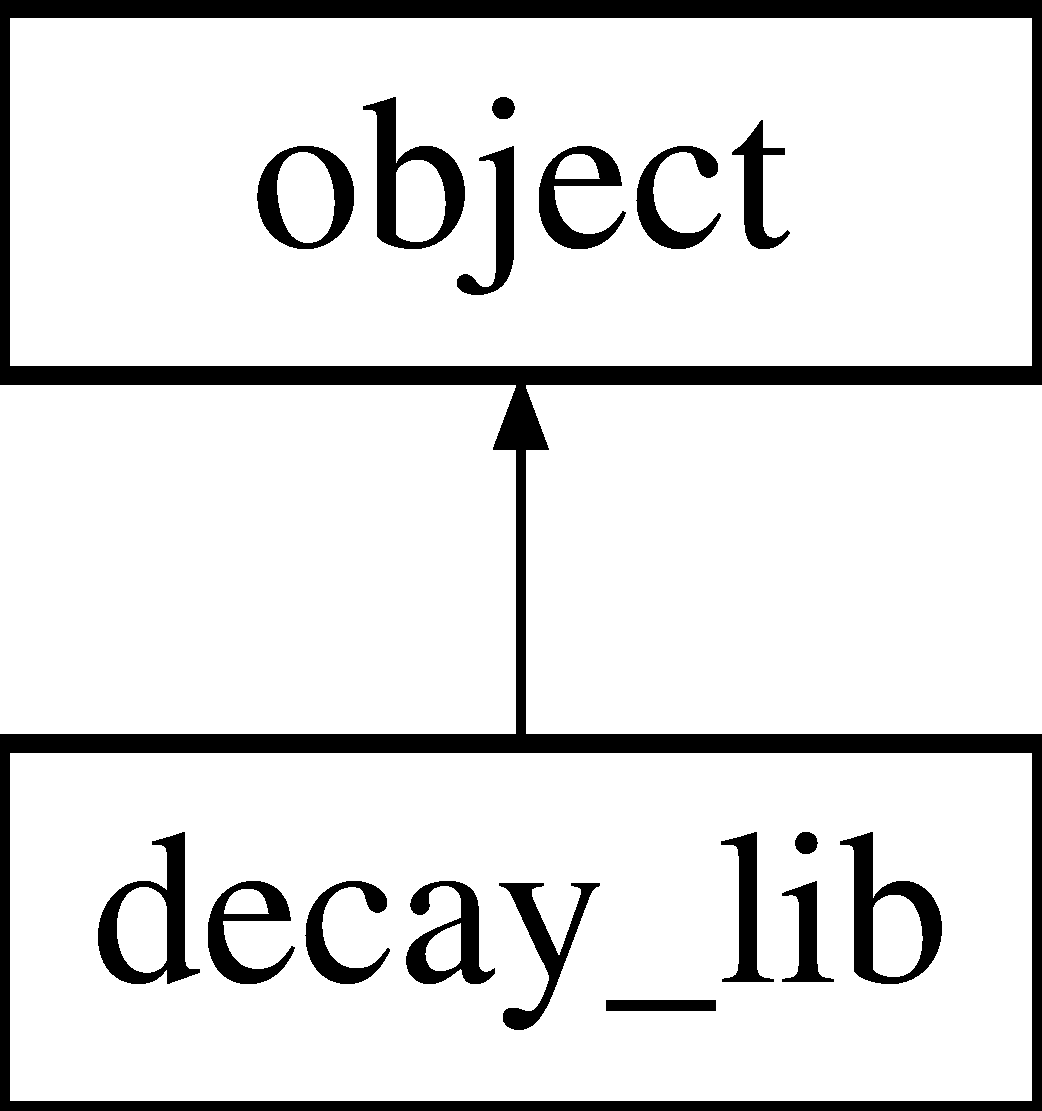
\includegraphics[height=2.000000cm]{classopenbu_1_1utils_1_1reactions__class_1_1decay__lib}
\end{center}
\end{figure}
\subsection*{Public Member Functions}
\subsection*{Private Attributes}


\subsection{Constructor \& Destructor Documentation}
\mbox{\Hypertarget{classopenbu_1_1utils_1_1reactions__class_1_1decay__lib_ae4664a4675345d114311cbd0ac402a0a}\label{classopenbu_1_1utils_1_1reactions__class_1_1decay__lib_ae4664a4675345d114311cbd0ac402a0a}} 
\index{openbu\+::utils\+::reactions\+\_\+class\+::decay\+\_\+lib@{openbu\+::utils\+::reactions\+\_\+class\+::decay\+\_\+lib}!\+\_\+\+\_\+init\+\_\+\+\_\+@{\+\_\+\+\_\+init\+\_\+\+\_\+}}
\index{\+\_\+\+\_\+init\+\_\+\+\_\+@{\+\_\+\+\_\+init\+\_\+\+\_\+}!openbu\+::utils\+::reactions\+\_\+class\+::decay\+\_\+lib@{openbu\+::utils\+::reactions\+\_\+class\+::decay\+\_\+lib}}
\subsubsection{\texorpdfstring{\+\_\+\+\_\+init\+\_\+\+\_\+()}{\_\_init\_\_()}}
{\footnotesize\ttfamily def \+\_\+\+\_\+init\+\_\+\+\_\+ (\begin{DoxyParamCaption}\item[{}]{self,  }\item[{}]{id\+\_\+number }\end{DoxyParamCaption})}



\subsection{Member Function Documentation}
\mbox{\Hypertarget{classopenbu_1_1utils_1_1reactions__class_1_1decay__lib_a794d3e0075d1c1b67e14535e6e62549a}\label{classopenbu_1_1utils_1_1reactions__class_1_1decay__lib_a794d3e0075d1c1b67e14535e6e62549a}} 
\index{openbu\+::utils\+::reactions\+\_\+class\+::decay\+\_\+lib@{openbu\+::utils\+::reactions\+\_\+class\+::decay\+\_\+lib}!add\+\_\+data@{add\+\_\+data}}
\index{add\+\_\+data@{add\+\_\+data}!openbu\+::utils\+::reactions\+\_\+class\+::decay\+\_\+lib@{openbu\+::utils\+::reactions\+\_\+class\+::decay\+\_\+lib}}
\subsubsection{\texorpdfstring{add\+\_\+data()}{add\_data()}}
{\footnotesize\ttfamily def add\+\_\+data (\begin{DoxyParamCaption}\item[{}]{self,  }\item[{}]{zamid,  }\item[{}]{kwargs }\end{DoxyParamCaption})}

\mbox{\Hypertarget{classopenbu_1_1utils_1_1reactions__class_1_1decay__lib_a3421376f5121500f9eb2b16677e8ed1e}\label{classopenbu_1_1utils_1_1reactions__class_1_1decay__lib_a3421376f5121500f9eb2b16677e8ed1e}} 
\index{openbu\+::utils\+::reactions\+\_\+class\+::decay\+\_\+lib@{openbu\+::utils\+::reactions\+\_\+class\+::decay\+\_\+lib}!create\+\_\+decay\+\_\+a@{create\+\_\+decay\+\_\+a}}
\index{create\+\_\+decay\+\_\+a@{create\+\_\+decay\+\_\+a}!openbu\+::utils\+::reactions\+\_\+class\+::decay\+\_\+lib@{openbu\+::utils\+::reactions\+\_\+class\+::decay\+\_\+lib}}
\subsubsection{\texorpdfstring{create\+\_\+decay\+\_\+a()}{create\_decay\_a()}}
{\footnotesize\ttfamily def create\+\_\+decay\+\_\+a (\begin{DoxyParamCaption}\item[{}]{self,  }\item[{}]{zamid,  }\item[{}]{dic }\end{DoxyParamCaption})}

\mbox{\Hypertarget{classopenbu_1_1utils_1_1reactions__class_1_1decay__lib_a0edaec2df85399cf219e36782994d43f}\label{classopenbu_1_1utils_1_1reactions__class_1_1decay__lib_a0edaec2df85399cf219e36782994d43f}} 
\index{openbu\+::utils\+::reactions\+\_\+class\+::decay\+\_\+lib@{openbu\+::utils\+::reactions\+\_\+class\+::decay\+\_\+lib}!create\+\_\+decay\+\_\+b@{create\+\_\+decay\+\_\+b}}
\index{create\+\_\+decay\+\_\+b@{create\+\_\+decay\+\_\+b}!openbu\+::utils\+::reactions\+\_\+class\+::decay\+\_\+lib@{openbu\+::utils\+::reactions\+\_\+class\+::decay\+\_\+lib}}
\subsubsection{\texorpdfstring{create\+\_\+decay\+\_\+b()}{create\_decay\_b()}}
{\footnotesize\ttfamily def create\+\_\+decay\+\_\+b (\begin{DoxyParamCaption}\item[{}]{self,  }\item[{}]{zamid,  }\item[{}]{dic }\end{DoxyParamCaption})}

\mbox{\Hypertarget{classopenbu_1_1utils_1_1reactions__class_1_1decay__lib_ab9d903431dc1a815d57cb09912e41e58}\label{classopenbu_1_1utils_1_1reactions__class_1_1decay__lib_ab9d903431dc1a815d57cb09912e41e58}} 
\index{openbu\+::utils\+::reactions\+\_\+class\+::decay\+\_\+lib@{openbu\+::utils\+::reactions\+\_\+class\+::decay\+\_\+lib}!decay\+\_\+a@{decay\+\_\+a}}
\index{decay\+\_\+a@{decay\+\_\+a}!openbu\+::utils\+::reactions\+\_\+class\+::decay\+\_\+lib@{openbu\+::utils\+::reactions\+\_\+class\+::decay\+\_\+lib}}
\subsubsection{\texorpdfstring{decay\+\_\+a()}{decay\_a()}}
{\footnotesize\ttfamily def decay\+\_\+a (\begin{DoxyParamCaption}\item[{}]{self }\end{DoxyParamCaption})}

\mbox{\Hypertarget{classopenbu_1_1utils_1_1reactions__class_1_1decay__lib_ade7165602b6bcdee1ed9b7256170379b}\label{classopenbu_1_1utils_1_1reactions__class_1_1decay__lib_ade7165602b6bcdee1ed9b7256170379b}} 
\index{openbu\+::utils\+::reactions\+\_\+class\+::decay\+\_\+lib@{openbu\+::utils\+::reactions\+\_\+class\+::decay\+\_\+lib}!decay\+\_\+b@{decay\+\_\+b}}
\index{decay\+\_\+b@{decay\+\_\+b}!openbu\+::utils\+::reactions\+\_\+class\+::decay\+\_\+lib@{openbu\+::utils\+::reactions\+\_\+class\+::decay\+\_\+lib}}
\subsubsection{\texorpdfstring{decay\+\_\+b()}{decay\_b()}}
{\footnotesize\ttfamily def decay\+\_\+b (\begin{DoxyParamCaption}\item[{}]{self }\end{DoxyParamCaption})}

\mbox{\Hypertarget{classopenbu_1_1utils_1_1reactions__class_1_1decay__lib_a80c88c99e45178594b9dc49b8852ee7e}\label{classopenbu_1_1utils_1_1reactions__class_1_1decay__lib_a80c88c99e45178594b9dc49b8852ee7e}} 
\index{openbu\+::utils\+::reactions\+\_\+class\+::decay\+\_\+lib@{openbu\+::utils\+::reactions\+\_\+class\+::decay\+\_\+lib}!dic@{dic}}
\index{dic@{dic}!openbu\+::utils\+::reactions\+\_\+class\+::decay\+\_\+lib@{openbu\+::utils\+::reactions\+\_\+class\+::decay\+\_\+lib}}
\subsubsection{\texorpdfstring{dic()}{dic()}}
{\footnotesize\ttfamily def dic (\begin{DoxyParamCaption}\item[{}]{self }\end{DoxyParamCaption})}



\subsection{Member Data Documentation}
\mbox{\Hypertarget{classopenbu_1_1utils_1_1reactions__class_1_1decay__lib_a1c2b24934d5eafbd256785b158a470a6}\label{classopenbu_1_1utils_1_1reactions__class_1_1decay__lib_a1c2b24934d5eafbd256785b158a470a6}} 
\index{openbu\+::utils\+::reactions\+\_\+class\+::decay\+\_\+lib@{openbu\+::utils\+::reactions\+\_\+class\+::decay\+\_\+lib}!\+\_\+decay\+\_\+a@{\+\_\+decay\+\_\+a}}
\index{\+\_\+decay\+\_\+a@{\+\_\+decay\+\_\+a}!openbu\+::utils\+::reactions\+\_\+class\+::decay\+\_\+lib@{openbu\+::utils\+::reactions\+\_\+class\+::decay\+\_\+lib}}
\subsubsection{\texorpdfstring{\+\_\+decay\+\_\+a}{\_decay\_a}}
{\footnotesize\ttfamily \+\_\+decay\+\_\+a\hspace{0.3cm}{\ttfamily [private]}}

\mbox{\Hypertarget{classopenbu_1_1utils_1_1reactions__class_1_1decay__lib_a74aadd383f9c57cbbfbb13289c5cc96f}\label{classopenbu_1_1utils_1_1reactions__class_1_1decay__lib_a74aadd383f9c57cbbfbb13289c5cc96f}} 
\index{openbu\+::utils\+::reactions\+\_\+class\+::decay\+\_\+lib@{openbu\+::utils\+::reactions\+\_\+class\+::decay\+\_\+lib}!\+\_\+decay\+\_\+b@{\+\_\+decay\+\_\+b}}
\index{\+\_\+decay\+\_\+b@{\+\_\+decay\+\_\+b}!openbu\+::utils\+::reactions\+\_\+class\+::decay\+\_\+lib@{openbu\+::utils\+::reactions\+\_\+class\+::decay\+\_\+lib}}
\subsubsection{\texorpdfstring{\+\_\+decay\+\_\+b}{\_decay\_b}}
{\footnotesize\ttfamily \+\_\+decay\+\_\+b\hspace{0.3cm}{\ttfamily [private]}}

\mbox{\Hypertarget{classopenbu_1_1utils_1_1reactions__class_1_1decay__lib_a67eb8fb1879c0d58ee16d390cfd736e4}\label{classopenbu_1_1utils_1_1reactions__class_1_1decay__lib_a67eb8fb1879c0d58ee16d390cfd736e4}} 
\index{openbu\+::utils\+::reactions\+\_\+class\+::decay\+\_\+lib@{openbu\+::utils\+::reactions\+\_\+class\+::decay\+\_\+lib}!\+\_\+dic@{\+\_\+dic}}
\index{\+\_\+dic@{\+\_\+dic}!openbu\+::utils\+::reactions\+\_\+class\+::decay\+\_\+lib@{openbu\+::utils\+::reactions\+\_\+class\+::decay\+\_\+lib}}
\subsubsection{\texorpdfstring{\+\_\+dic}{\_dic}}
{\footnotesize\ttfamily \+\_\+dic\hspace{0.3cm}{\ttfamily [private]}}

\mbox{\Hypertarget{classopenbu_1_1utils_1_1reactions__class_1_1decay__lib_aa1313b5b76f38d461c99c9a42b437f74}\label{classopenbu_1_1utils_1_1reactions__class_1_1decay__lib_aa1313b5b76f38d461c99c9a42b437f74}} 
\index{openbu\+::utils\+::reactions\+\_\+class\+::decay\+\_\+lib@{openbu\+::utils\+::reactions\+\_\+class\+::decay\+\_\+lib}!\+\_\+id@{\+\_\+id}}
\index{\+\_\+id@{\+\_\+id}!openbu\+::utils\+::reactions\+\_\+class\+::decay\+\_\+lib@{openbu\+::utils\+::reactions\+\_\+class\+::decay\+\_\+lib}}
\subsubsection{\texorpdfstring{\+\_\+id}{\_id}}
{\footnotesize\ttfamily \+\_\+id\hspace{0.3cm}{\ttfamily [private]}}



The documentation for this class was generated from the following file\+:\begin{DoxyCompactItemize}
\item 
/\+Users/mouginot/work/app/\+Open\+B\+U/openbu/utils/\mbox{\hyperlink{reactions__class_8py}{reactions\+\_\+class.\+py}}\end{DoxyCompactItemize}

\hypertarget{classopenbu_1_1utils_1_1functions_1_1_empty__argument}{}\doxysection{Empty\+\_\+argument Class Reference}
\label{classopenbu_1_1utils_1_1functions_1_1_empty__argument}\index{Empty\_argument@{Empty\_argument}}
Inheritance diagram for Empty\+\_\+argument\+:\begin{figure}[H]
\begin{center}
\leavevmode
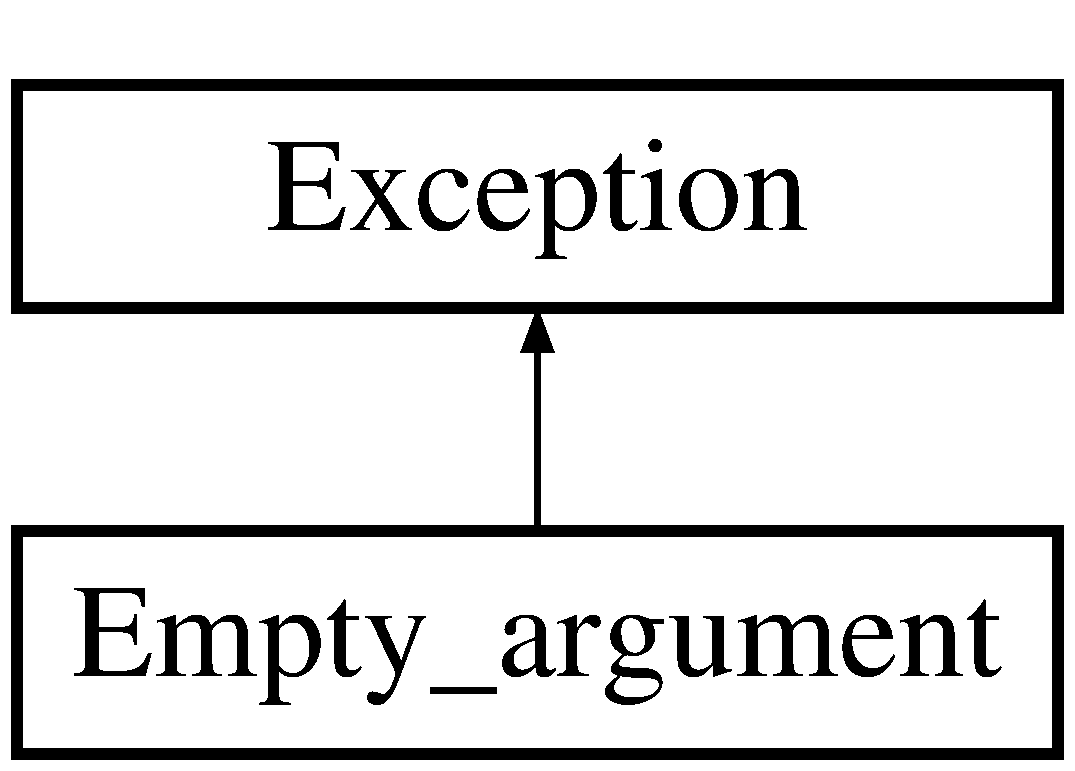
\includegraphics[height=2.000000cm]{classopenbu_1_1utils_1_1functions_1_1_empty__argument}
\end{center}
\end{figure}


\doxysubsection{Detailed Description}
\begin{DoxyVerb}Raise when the user calls decay_halflife_conv without entering any argument \end{DoxyVerb}
 

The documentation for this class was generated from the following file\+:\begin{DoxyCompactItemize}
\item 
utils/functions.\+py\end{DoxyCompactItemize}

\hypertarget{classopenbu_1_1utils_1_1reactions__class_1_1_empty__data}{}\section{Empty\+\_\+data Class Reference}
\label{classopenbu_1_1utils_1_1reactions__class_1_1_empty__data}\index{Empty\+\_\+data@{Empty\+\_\+data}}
Inheritance diagram for Empty\+\_\+data\+:\begin{figure}[H]
\begin{center}
\leavevmode
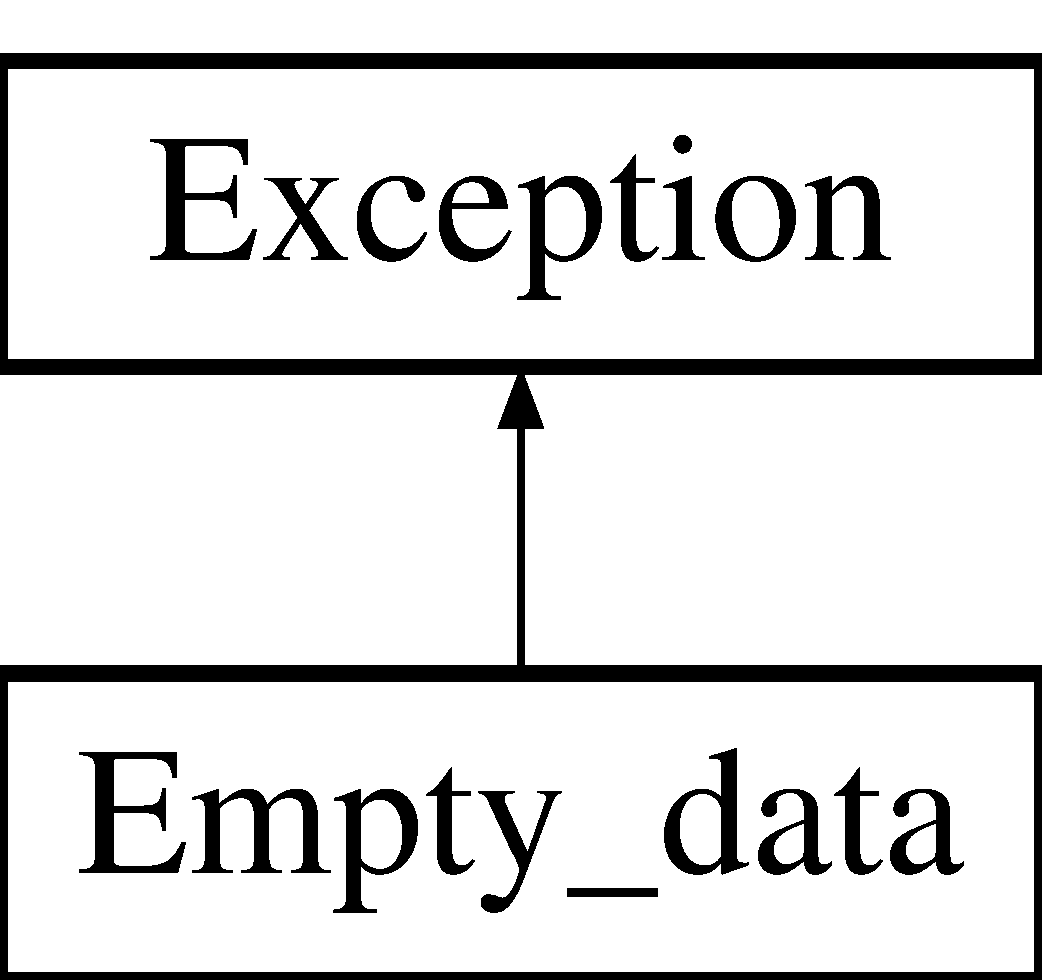
\includegraphics[height=2.000000cm]{classopenbu_1_1utils_1_1reactions__class_1_1_empty__data}
\end{center}
\end{figure}


\subsection{Detailed Description}
\begin{DoxyVerb}Raise when the user does not enter any data while add_data has been called for a nuclide\end{DoxyVerb}
 

The documentation for this class was generated from the following file\+:\begin{DoxyCompactItemize}
\item 
/\+Users/mouginot/work/app/\+Open\+B\+U/openbu/utils/reactions\+\_\+class.\+py\end{DoxyCompactItemize}

\hypertarget{classopenbu_1_1utils_1_1reactions__class_1_1fy__lib}{}\section{fy\+\_\+lib Class Reference}
\label{classopenbu_1_1utils_1_1reactions__class_1_1fy__lib}\index{fy\+\_\+lib@{fy\+\_\+lib}}
Inheritance diagram for fy\+\_\+lib\+:\begin{figure}[H]
\begin{center}
\leavevmode
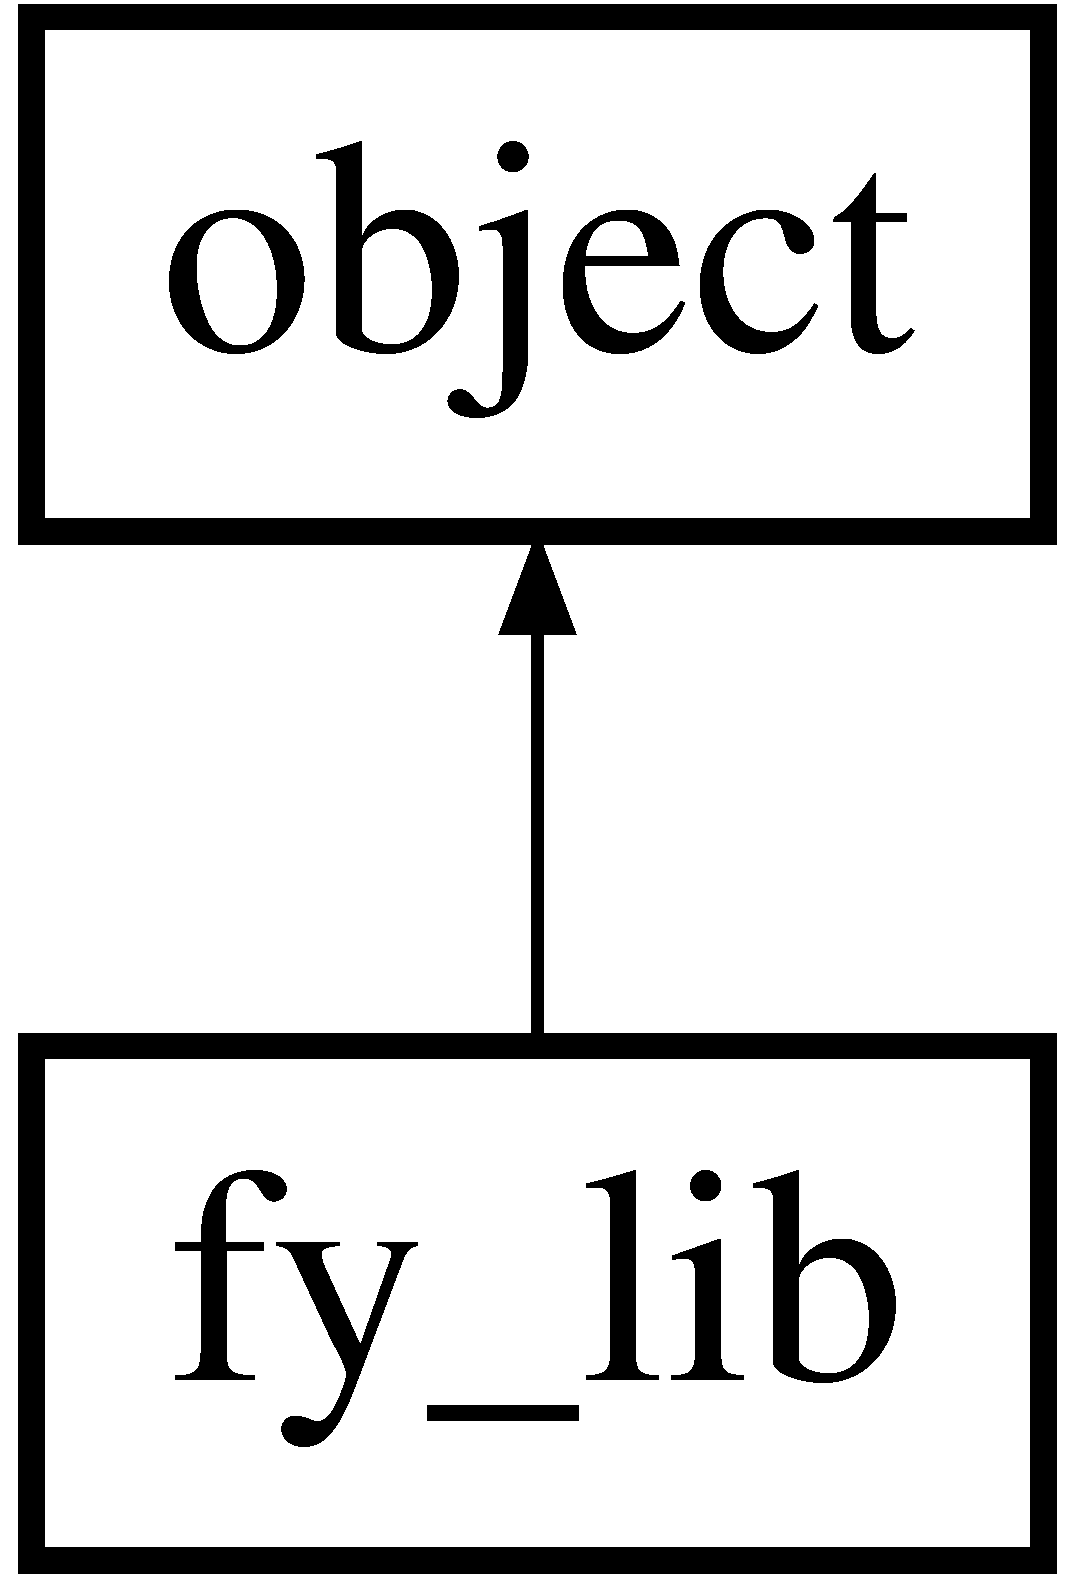
\includegraphics[height=2.000000cm]{classopenbu_1_1utils_1_1reactions__class_1_1fy__lib}
\end{center}
\end{figure}
\subsection*{Public Member Functions}
\subsection*{Private Attributes}


\subsection{Constructor \& Destructor Documentation}
\mbox{\Hypertarget{classopenbu_1_1utils_1_1reactions__class_1_1fy__lib_ae4664a4675345d114311cbd0ac402a0a}\label{classopenbu_1_1utils_1_1reactions__class_1_1fy__lib_ae4664a4675345d114311cbd0ac402a0a}} 
\index{openbu\+::utils\+::reactions\+\_\+class\+::fy\+\_\+lib@{openbu\+::utils\+::reactions\+\_\+class\+::fy\+\_\+lib}!\+\_\+\+\_\+init\+\_\+\+\_\+@{\+\_\+\+\_\+init\+\_\+\+\_\+}}
\index{\+\_\+\+\_\+init\+\_\+\+\_\+@{\+\_\+\+\_\+init\+\_\+\+\_\+}!openbu\+::utils\+::reactions\+\_\+class\+::fy\+\_\+lib@{openbu\+::utils\+::reactions\+\_\+class\+::fy\+\_\+lib}}
\subsubsection{\texorpdfstring{\+\_\+\+\_\+init\+\_\+\+\_\+()}{\_\_init\_\_()}}
{\footnotesize\ttfamily def \+\_\+\+\_\+init\+\_\+\+\_\+ (\begin{DoxyParamCaption}\item[{}]{self,  }\item[{}]{id\+\_\+number }\end{DoxyParamCaption})}



\subsection{Member Function Documentation}
\mbox{\Hypertarget{classopenbu_1_1utils_1_1reactions__class_1_1fy__lib_ab51433137df38fc8bd763ceda7026af2}\label{classopenbu_1_1utils_1_1reactions__class_1_1fy__lib_ab51433137df38fc8bd763ceda7026af2}} 
\index{openbu\+::utils\+::reactions\+\_\+class\+::fy\+\_\+lib@{openbu\+::utils\+::reactions\+\_\+class\+::fy\+\_\+lib}!add\+\_\+data@{add\+\_\+data}}
\index{add\+\_\+data@{add\+\_\+data}!openbu\+::utils\+::reactions\+\_\+class\+::fy\+\_\+lib@{openbu\+::utils\+::reactions\+\_\+class\+::fy\+\_\+lib}}
\subsubsection{\texorpdfstring{add\+\_\+data()}{add\_data()}}
{\footnotesize\ttfamily def add\+\_\+data (\begin{DoxyParamCaption}\item[{}]{self,  }\item[{}]{zamid,  }\item[{}]{dic }\end{DoxyParamCaption})}

\mbox{\Hypertarget{classopenbu_1_1utils_1_1reactions__class_1_1fy__lib_a8b75ace3008810461600cc7df511303b}\label{classopenbu_1_1utils_1_1reactions__class_1_1fy__lib_a8b75ace3008810461600cc7df511303b}} 
\index{openbu\+::utils\+::reactions\+\_\+class\+::fy\+\_\+lib@{openbu\+::utils\+::reactions\+\_\+class\+::fy\+\_\+lib}!fy@{fy}}
\index{fy@{fy}!openbu\+::utils\+::reactions\+\_\+class\+::fy\+\_\+lib@{openbu\+::utils\+::reactions\+\_\+class\+::fy\+\_\+lib}}
\subsubsection{\texorpdfstring{fy()}{fy()}}
{\footnotesize\ttfamily def fy (\begin{DoxyParamCaption}\item[{}]{self }\end{DoxyParamCaption})}



\subsection{Member Data Documentation}
\mbox{\Hypertarget{classopenbu_1_1utils_1_1reactions__class_1_1fy__lib_a67eb8fb1879c0d58ee16d390cfd736e4}\label{classopenbu_1_1utils_1_1reactions__class_1_1fy__lib_a67eb8fb1879c0d58ee16d390cfd736e4}} 
\index{openbu\+::utils\+::reactions\+\_\+class\+::fy\+\_\+lib@{openbu\+::utils\+::reactions\+\_\+class\+::fy\+\_\+lib}!\+\_\+dic@{\+\_\+dic}}
\index{\+\_\+dic@{\+\_\+dic}!openbu\+::utils\+::reactions\+\_\+class\+::fy\+\_\+lib@{openbu\+::utils\+::reactions\+\_\+class\+::fy\+\_\+lib}}
\subsubsection{\texorpdfstring{\+\_\+dic}{\_dic}}
{\footnotesize\ttfamily \+\_\+dic\hspace{0.3cm}{\ttfamily [private]}}

\mbox{\Hypertarget{classopenbu_1_1utils_1_1reactions__class_1_1fy__lib_a47fe437d4dacfd52d3296390e1bd67f8}\label{classopenbu_1_1utils_1_1reactions__class_1_1fy__lib_a47fe437d4dacfd52d3296390e1bd67f8}} 
\index{openbu\+::utils\+::reactions\+\_\+class\+::fy\+\_\+lib@{openbu\+::utils\+::reactions\+\_\+class\+::fy\+\_\+lib}!\+\_\+fy@{\+\_\+fy}}
\index{\+\_\+fy@{\+\_\+fy}!openbu\+::utils\+::reactions\+\_\+class\+::fy\+\_\+lib@{openbu\+::utils\+::reactions\+\_\+class\+::fy\+\_\+lib}}
\subsubsection{\texorpdfstring{\+\_\+fy}{\_fy}}
{\footnotesize\ttfamily \+\_\+fy\hspace{0.3cm}{\ttfamily [private]}}

\mbox{\Hypertarget{classopenbu_1_1utils_1_1reactions__class_1_1fy__lib_aa1313b5b76f38d461c99c9a42b437f74}\label{classopenbu_1_1utils_1_1reactions__class_1_1fy__lib_aa1313b5b76f38d461c99c9a42b437f74}} 
\index{openbu\+::utils\+::reactions\+\_\+class\+::fy\+\_\+lib@{openbu\+::utils\+::reactions\+\_\+class\+::fy\+\_\+lib}!\+\_\+id@{\+\_\+id}}
\index{\+\_\+id@{\+\_\+id}!openbu\+::utils\+::reactions\+\_\+class\+::fy\+\_\+lib@{openbu\+::utils\+::reactions\+\_\+class\+::fy\+\_\+lib}}
\subsubsection{\texorpdfstring{\+\_\+id}{\_id}}
{\footnotesize\ttfamily \+\_\+id\hspace{0.3cm}{\ttfamily [private]}}



The documentation for this class was generated from the following file\+:\begin{DoxyCompactItemize}
\item 
/\+Users/mouginot/work/app/\+Open\+B\+U/openbu/utils/\mbox{\hyperlink{reactions__class_8py}{reactions\+\_\+class.\+py}}\end{DoxyCompactItemize}

\hypertarget{classopenbu_1_1passport_1_1_incorrect__nuc__id}{}\section{Incorrect\+\_\+nuc\+\_\+id Class Reference}
\label{classopenbu_1_1passport_1_1_incorrect__nuc__id}\index{Incorrect\+\_\+nuc\+\_\+id@{Incorrect\+\_\+nuc\+\_\+id}}
Inheritance diagram for Incorrect\+\_\+nuc\+\_\+id\+:\begin{figure}[H]
\begin{center}
\leavevmode
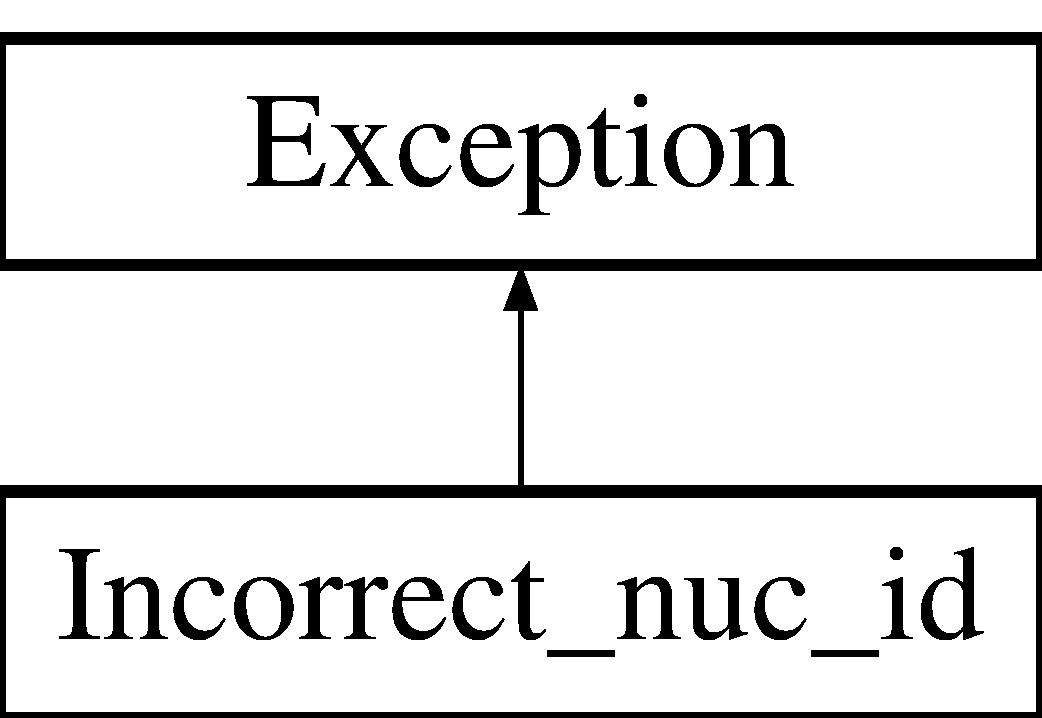
\includegraphics[height=2.000000cm]{classopenbu_1_1passport_1_1_incorrect__nuc__id}
\end{center}
\end{figure}


\subsection{Detailed Description}
\begin{DoxyVerb}Raise when the id input format in passport instantiation is incorrect\end{DoxyVerb}
 

The documentation for this class was generated from the following file\+:\begin{DoxyCompactItemize}
\item 
/\+Users/mouginot/work/app/\+Open\+B\+U/openbu/\mbox{\hyperlink{passport_8py}{passport.\+py}}\end{DoxyCompactItemize}

\hypertarget{classopenbu_1_1cell_1_1_initial__nucl__not__in___nucl__set}{}\section{Initial\+\_\+nucl\+\_\+not\+\_\+in\+\_\+\+Nucl\+\_\+set Class Reference}
\label{classopenbu_1_1cell_1_1_initial__nucl__not__in___nucl__set}\index{Initial\+\_\+nucl\+\_\+not\+\_\+in\+\_\+\+Nucl\+\_\+set@{Initial\+\_\+nucl\+\_\+not\+\_\+in\+\_\+\+Nucl\+\_\+set}}
Inheritance diagram for Initial\+\_\+nucl\+\_\+not\+\_\+in\+\_\+\+Nucl\+\_\+set\+:\begin{figure}[H]
\begin{center}
\leavevmode
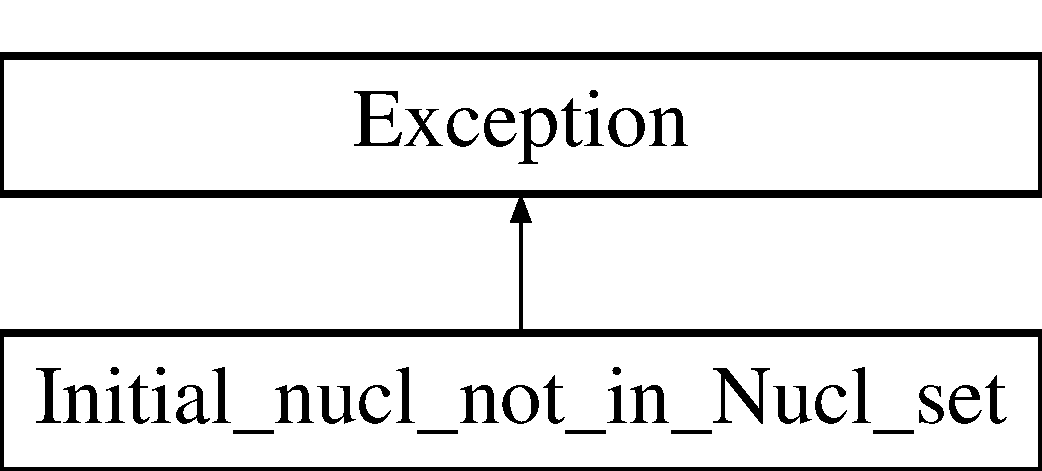
\includegraphics[height=2.000000cm]{classopenbu_1_1cell_1_1_initial__nucl__not__in___nucl__set}
\end{center}
\end{figure}


\subsection{Detailed Description}
\begin{DoxyVerb}Raise when the user forgot to set the initial nuclide of the cell and tries to burn cell\end{DoxyVerb}
 

The documentation for this class was generated from the following file\+:\begin{DoxyCompactItemize}
\item 
/\+Users/mouginot/work/app/\+Open\+B\+U/openbu/\mbox{\hyperlink{cell_8py}{cell.\+py}}\end{DoxyCompactItemize}

\hypertarget{classopenbu_1_1cell_1_1_initial__nucl__not__set}{}\doxysection{Initial\+\_\+nucl\+\_\+not\+\_\+set Class Reference}
\label{classopenbu_1_1cell_1_1_initial__nucl__not__set}\index{Initial\_nucl\_not\_set@{Initial\_nucl\_not\_set}}
Inheritance diagram for Initial\+\_\+nucl\+\_\+not\+\_\+set\+:\begin{figure}[H]
\begin{center}
\leavevmode
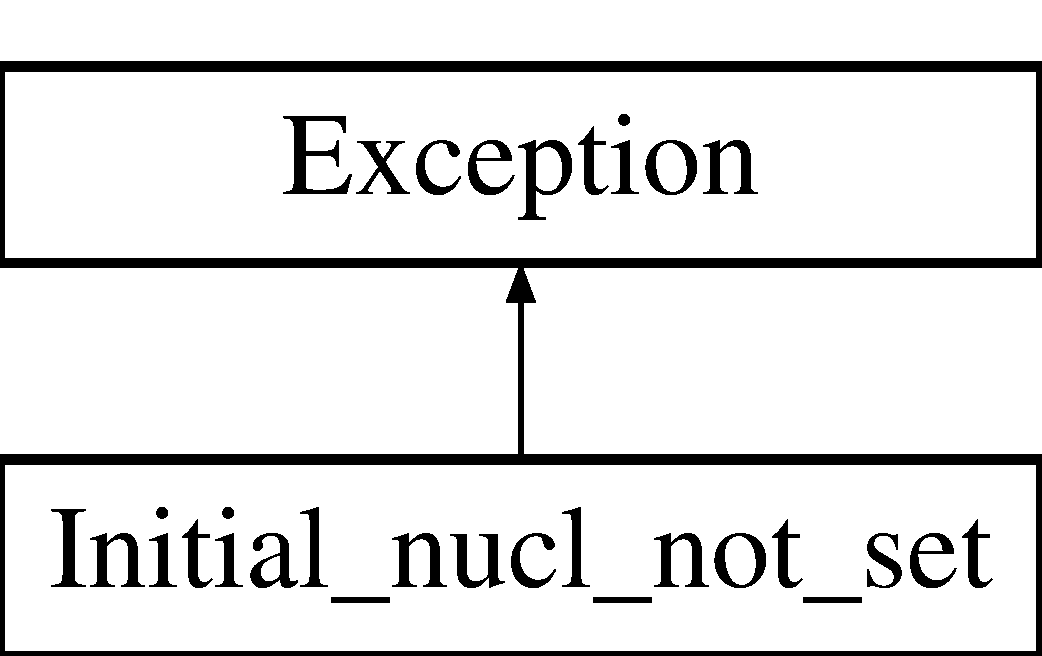
\includegraphics[height=2.000000cm]{classopenbu_1_1cell_1_1_initial__nucl__not__set}
\end{center}
\end{figure}


\doxysubsection{Detailed Description}
\begin{DoxyVerb}Raise when the user forgot to set the initial nuclide of the cell and tries to burn cell\end{DoxyVerb}
 

The documentation for this class was generated from the following file\+:\begin{DoxyCompactItemize}
\item 
cell.\+py\end{DoxyCompactItemize}

\hypertarget{classopenbu_1_1couple_1_1couple__openmc_1_1_initial__nuclides__not__in__nuclide__list}{}\section{Initial\+\_\+nuclides\+\_\+not\+\_\+in\+\_\+nuclide\+\_\+list Class Reference}
\label{classopenbu_1_1couple_1_1couple__openmc_1_1_initial__nuclides__not__in__nuclide__list}\index{Initial\+\_\+nuclides\+\_\+not\+\_\+in\+\_\+nuclide\+\_\+list@{Initial\+\_\+nuclides\+\_\+not\+\_\+in\+\_\+nuclide\+\_\+list}}
Inheritance diagram for Initial\+\_\+nuclides\+\_\+not\+\_\+in\+\_\+nuclide\+\_\+list\+:\begin{figure}[H]
\begin{center}
\leavevmode
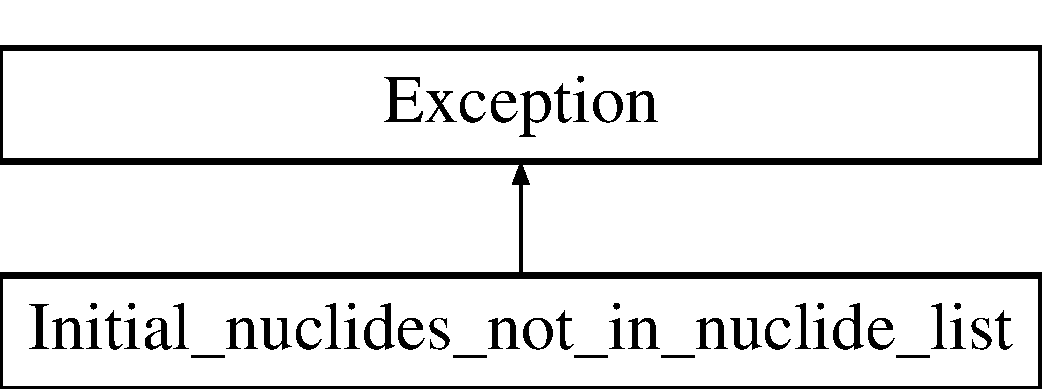
\includegraphics[height=2.000000cm]{classopenbu_1_1couple_1_1couple__openmc_1_1_initial__nuclides__not__in__nuclide__list}
\end{center}
\end{figure}


\subsection{Detailed Description}
\begin{DoxyVerb}Raise when some initial nuclides are not included in nucl_list \end{DoxyVerb}
 

The documentation for this class was generated from the following file\+:\begin{DoxyCompactItemize}
\item 
/\+Users/mouginot/work/app/\+Open\+B\+U/openbu/couple/\mbox{\hyperlink{couple__openmc_8py}{couple\+\_\+openmc.\+py}}\end{DoxyCompactItemize}

\hypertarget{classopenbu_1_1input_1_1_input}{}\doxysection{Input Class Reference}
\label{classopenbu_1_1input_1_1_input}\index{Input@{Input}}
Inheritance diagram for Input\+:\begin{figure}[H]
\begin{center}
\leavevmode
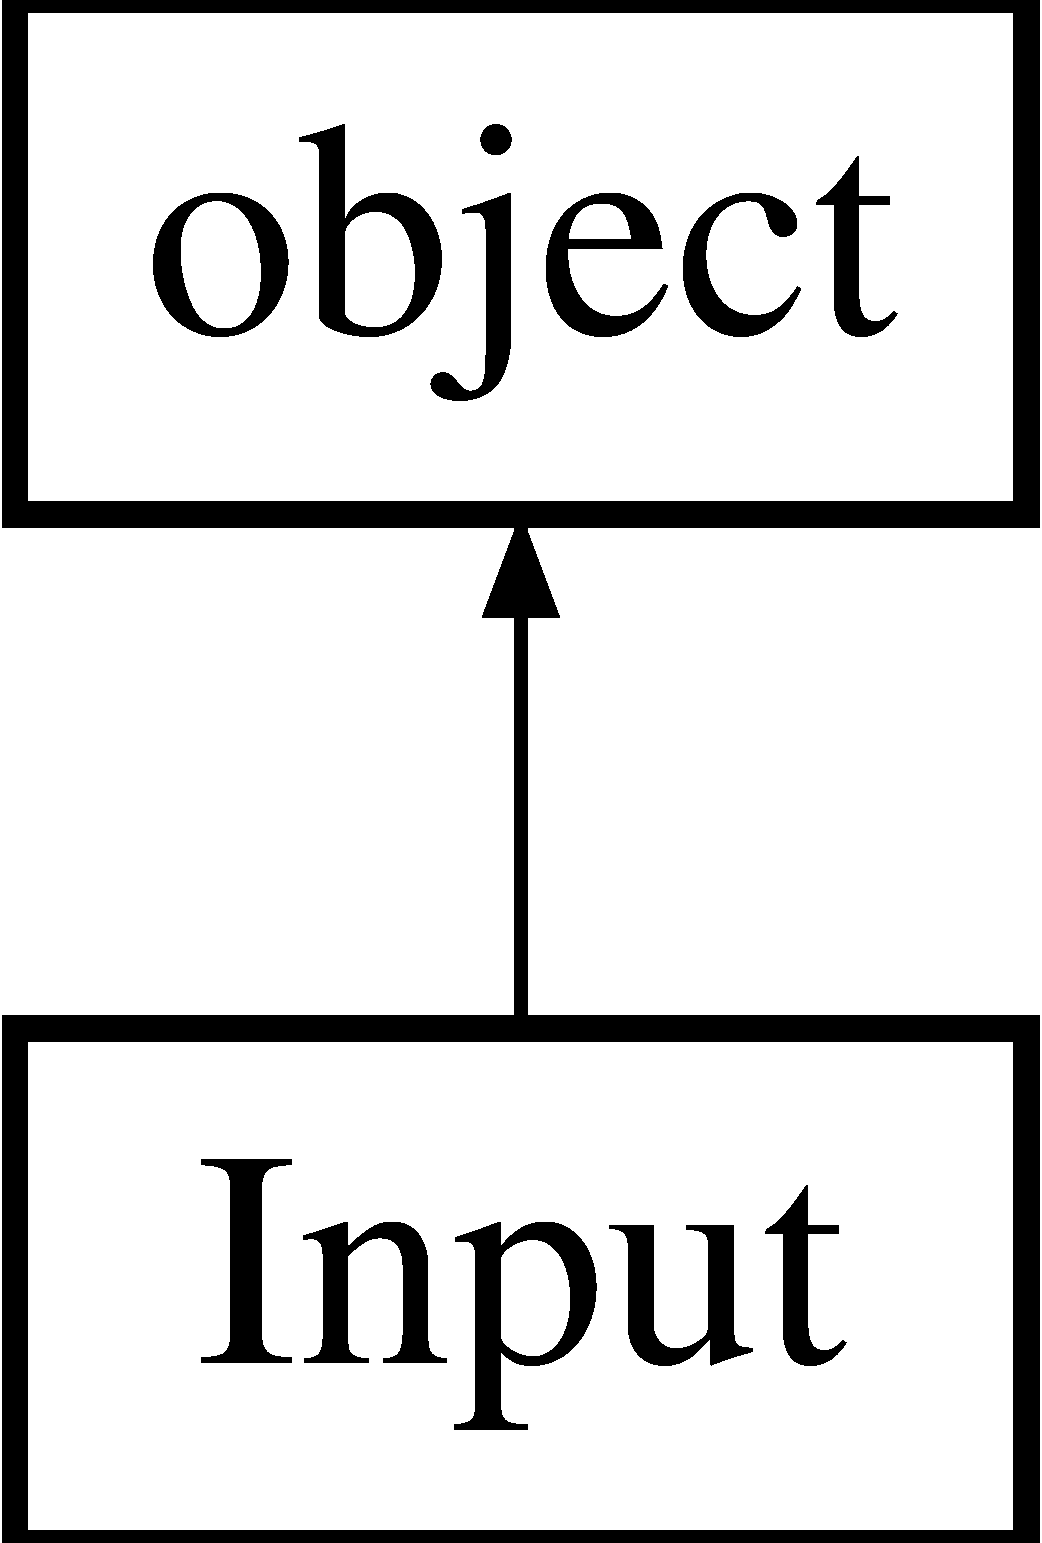
\includegraphics[height=2.000000cm]{classopenbu_1_1input_1_1_input}
\end{center}
\end{figure}
\doxysubsection*{Public Member Functions}
\doxysubsection*{Public Attributes}
\doxysubsection*{Private Member Functions}
\doxysubsection*{Private Attributes}
\doxysubsection*{Static Private Attributes}


\doxysubsection{Detailed Description}
\begin{DoxyVerb}input reads, stores and process the input data in the input file provided by the user\end{DoxyVerb}
 

\doxysubsection{Member Function Documentation}
\mbox{\Hypertarget{classopenbu_1_1input_1_1_input_aec654cc5b1c47a58ce5dd1de926b8c17}\label{classopenbu_1_1input_1_1_input_aec654cc5b1c47a58ce5dd1de926b8c17}} 
\index{Input@{Input}!cell\_id\_list@{cell\_id\_list}}
\index{cell\_id\_list@{cell\_id\_list}!Input@{Input}}
\doxysubsubsection{\texorpdfstring{cell\_id\_list()}{cell\_id\_list()}}
{\footnotesize\ttfamily def cell\+\_\+id\+\_\+list (\begin{DoxyParamCaption}\item[{}]{self }\end{DoxyParamCaption})}

\begin{DoxyVerb}Returns the absolute values of the decay constant of the nuclide\end{DoxyVerb}
 \mbox{\Hypertarget{classopenbu_1_1input_1_1_input_ada83a03c99c1587bee0ffb75e04f0589}\label{classopenbu_1_1input_1_1_input_ada83a03c99c1587bee0ffb75e04f0589}} 
\index{Input@{Input}!cells@{cells}}
\index{cells@{cells}!Input@{Input}}
\doxysubsubsection{\texorpdfstring{cells()}{cells()}}
{\footnotesize\ttfamily def cells (\begin{DoxyParamCaption}\item[{}]{self }\end{DoxyParamCaption})}

\begin{DoxyVerb}Returns the absolute values of the decay constant of the nuclide\end{DoxyVerb}
 \mbox{\Hypertarget{classopenbu_1_1input_1_1_input_a7c74249450d6c2107885b03f5328ca75}\label{classopenbu_1_1input_1_1_input_a7c74249450d6c2107885b03f5328ca75}} 
\index{Input@{Input}!lib@{lib}}
\index{lib@{lib}!Input@{Input}}
\doxysubsubsection{\texorpdfstring{lib()}{lib()}}
{\footnotesize\ttfamily def lib (\begin{DoxyParamCaption}\item[{}]{self }\end{DoxyParamCaption})}

\begin{DoxyVerb}Returns the absolute values of the decay constant of the nuclide\end{DoxyVerb}
 \mbox{\Hypertarget{classopenbu_1_1input_1_1_input_a6ef2947c0b15938b4f351065ee10dcc9}\label{classopenbu_1_1input_1_1_input_a6ef2947c0b15938b4f351065ee10dcc9}} 
\index{Input@{Input}!mode@{mode}}
\index{mode@{mode}!Input@{Input}}
\doxysubsubsection{\texorpdfstring{mode()}{mode()}}
{\footnotesize\ttfamily def mode (\begin{DoxyParamCaption}\item[{}]{self }\end{DoxyParamCaption})}

\begin{DoxyVerb}Returns the absolute values of the decay constant of the nuclide\end{DoxyVerb}
 

The documentation for this class was generated from the following file\+:\begin{DoxyCompactItemize}
\item 
input.\+py\end{DoxyCompactItemize}

\hypertarget{classopenbu_1_1utils_1_1functions_1_1_midpoint_normalize}{}\section{Midpoint\+Normalize Class Reference}
\label{classopenbu_1_1utils_1_1functions_1_1_midpoint_normalize}\index{Midpoint\+Normalize@{Midpoint\+Normalize}}
Inheritance diagram for Midpoint\+Normalize\+:\begin{figure}[H]
\begin{center}
\leavevmode
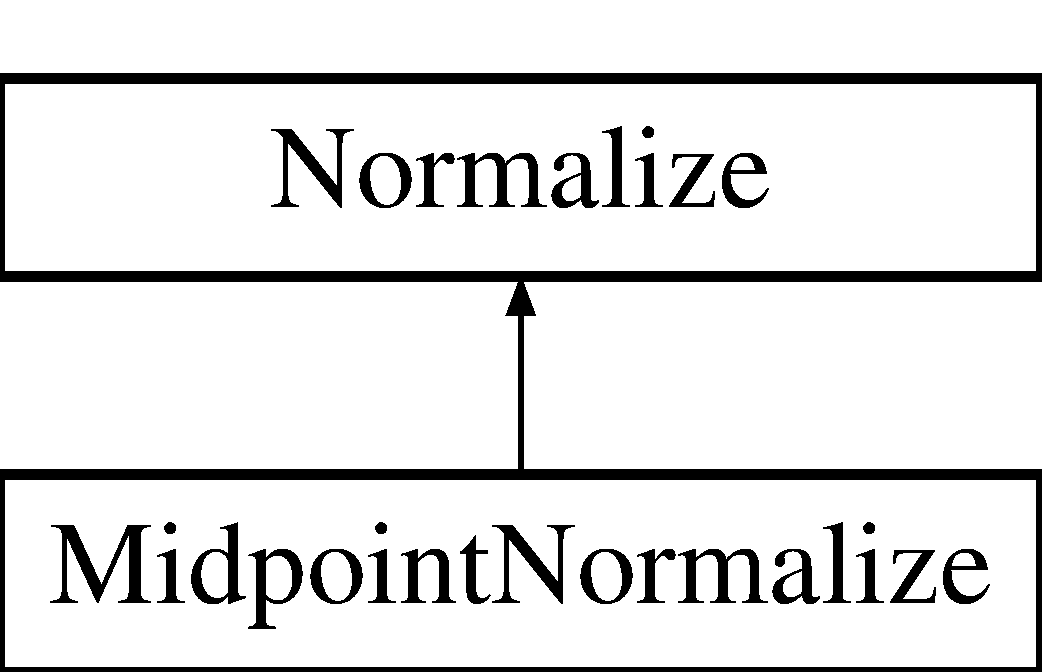
\includegraphics[height=2.000000cm]{classopenbu_1_1utils_1_1functions_1_1_midpoint_normalize}
\end{center}
\end{figure}
\subsection*{Public Member Functions}
\subsection*{Public Attributes}


\subsection{Detailed Description}
\begin{DoxyVerb}Normalise the colorbar so that diverging bars work there way either side from a prescribed midpoint value)

e.g. im=ax1.imshow(array, norm=MidpointNormalize(midpoint=0.,vmin=-100, vmax=100))
\end{DoxyVerb}
 

\subsection{Constructor \& Destructor Documentation}
\mbox{\Hypertarget{classopenbu_1_1utils_1_1functions_1_1_midpoint_normalize_a87831fcbb459c9db73a8c7ce1d07a760}\label{classopenbu_1_1utils_1_1functions_1_1_midpoint_normalize_a87831fcbb459c9db73a8c7ce1d07a760}} 
\index{openbu\+::utils\+::functions\+::\+Midpoint\+Normalize@{openbu\+::utils\+::functions\+::\+Midpoint\+Normalize}!\+\_\+\+\_\+init\+\_\+\+\_\+@{\+\_\+\+\_\+init\+\_\+\+\_\+}}
\index{\+\_\+\+\_\+init\+\_\+\+\_\+@{\+\_\+\+\_\+init\+\_\+\+\_\+}!openbu\+::utils\+::functions\+::\+Midpoint\+Normalize@{openbu\+::utils\+::functions\+::\+Midpoint\+Normalize}}
\subsubsection{\texorpdfstring{\+\_\+\+\_\+init\+\_\+\+\_\+()}{\_\_init\_\_()}}
{\footnotesize\ttfamily def \+\_\+\+\_\+init\+\_\+\+\_\+ (\begin{DoxyParamCaption}\item[{}]{self,  }\item[{}]{vmin = {\ttfamily None},  }\item[{}]{vmax = {\ttfamily None},  }\item[{}]{midpoint = {\ttfamily None},  }\item[{}]{clip = {\ttfamily False} }\end{DoxyParamCaption})}



\subsection{Member Function Documentation}
\mbox{\Hypertarget{classopenbu_1_1utils_1_1functions_1_1_midpoint_normalize_aa6cce7eb63fb71fe8f5f1bc150371618}\label{classopenbu_1_1utils_1_1functions_1_1_midpoint_normalize_aa6cce7eb63fb71fe8f5f1bc150371618}} 
\index{openbu\+::utils\+::functions\+::\+Midpoint\+Normalize@{openbu\+::utils\+::functions\+::\+Midpoint\+Normalize}!\+\_\+\+\_\+call\+\_\+\+\_\+@{\+\_\+\+\_\+call\+\_\+\+\_\+}}
\index{\+\_\+\+\_\+call\+\_\+\+\_\+@{\+\_\+\+\_\+call\+\_\+\+\_\+}!openbu\+::utils\+::functions\+::\+Midpoint\+Normalize@{openbu\+::utils\+::functions\+::\+Midpoint\+Normalize}}
\subsubsection{\texorpdfstring{\+\_\+\+\_\+call\+\_\+\+\_\+()}{\_\_call\_\_()}}
{\footnotesize\ttfamily def \+\_\+\+\_\+call\+\_\+\+\_\+ (\begin{DoxyParamCaption}\item[{}]{self,  }\item[{}]{value,  }\item[{}]{clip = {\ttfamily None} }\end{DoxyParamCaption})}



\subsection{Member Data Documentation}
\mbox{\Hypertarget{classopenbu_1_1utils_1_1functions_1_1_midpoint_normalize_af53e0eb961b2050b7ae1f7994bfed8ff}\label{classopenbu_1_1utils_1_1functions_1_1_midpoint_normalize_af53e0eb961b2050b7ae1f7994bfed8ff}} 
\index{openbu\+::utils\+::functions\+::\+Midpoint\+Normalize@{openbu\+::utils\+::functions\+::\+Midpoint\+Normalize}!midpoint@{midpoint}}
\index{midpoint@{midpoint}!openbu\+::utils\+::functions\+::\+Midpoint\+Normalize@{openbu\+::utils\+::functions\+::\+Midpoint\+Normalize}}
\subsubsection{\texorpdfstring{midpoint}{midpoint}}
{\footnotesize\ttfamily midpoint}



The documentation for this class was generated from the following file\+:\begin{DoxyCompactItemize}
\item 
/\+Users/mouginot/work/app/\+Open\+B\+U/openbu/utils/\mbox{\hyperlink{utils_2functions_8py}{functions.\+py}}\end{DoxyCompactItemize}

\hypertarget{classopenbu_1_1passlist_1_1_neg__decay}{}\doxysection{Neg\+\_\+decay Class Reference}
\label{classopenbu_1_1passlist_1_1_neg__decay}\index{Neg\_decay@{Neg\_decay}}
Inheritance diagram for Neg\+\_\+decay\+:\begin{figure}[H]
\begin{center}
\leavevmode
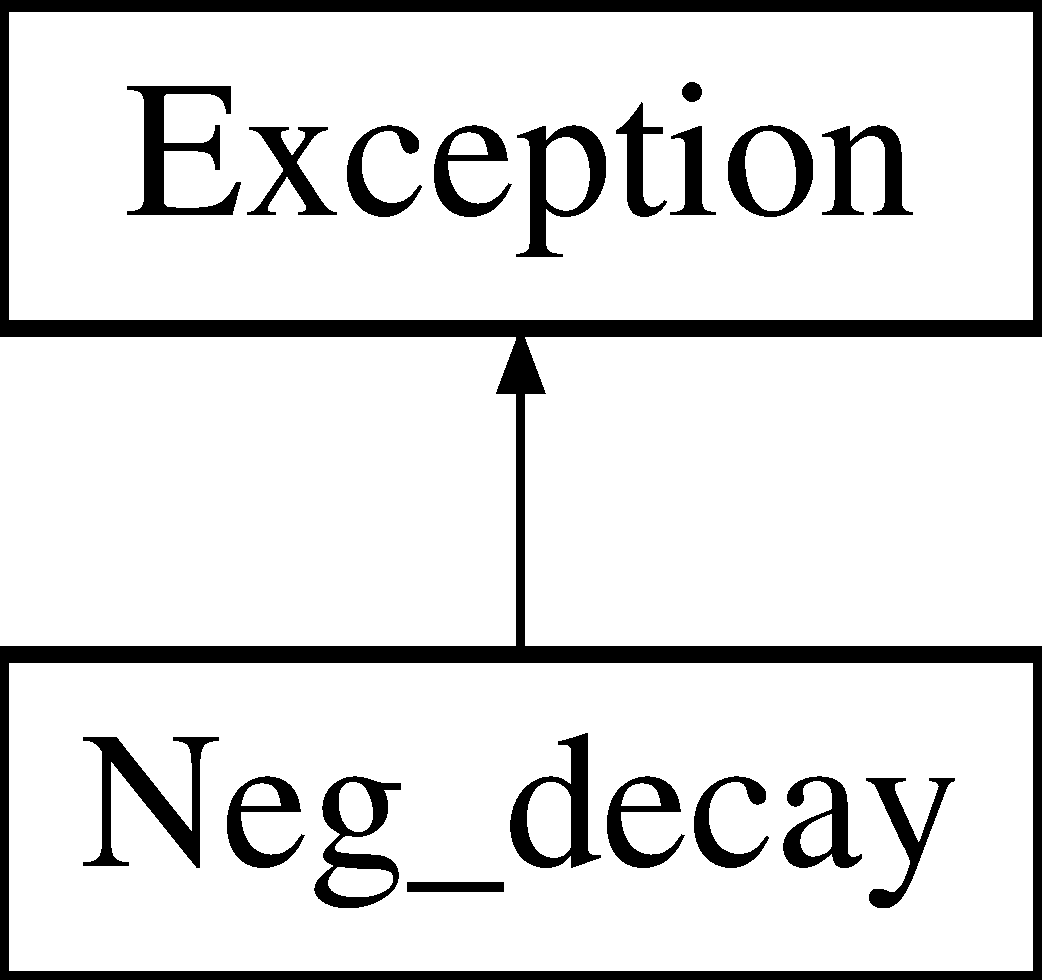
\includegraphics[height=2.000000cm]{classopenbu_1_1passlist_1_1_neg__decay}
\end{center}
\end{figure}


\doxysubsection{Detailed Description}
\begin{DoxyVerb}Raise when a negative decay constant is found\end{DoxyVerb}
 

The documentation for this class was generated from the following file\+:\begin{DoxyCompactItemize}
\item 
passlist.\+py\end{DoxyCompactItemize}

\hypertarget{classopenbu_1_1passlist_1_1_neg__xs}{}\doxysection{Neg\+\_\+xs Class Reference}
\label{classopenbu_1_1passlist_1_1_neg__xs}\index{Neg\_xs@{Neg\_xs}}
Inheritance diagram for Neg\+\_\+xs\+:\begin{figure}[H]
\begin{center}
\leavevmode
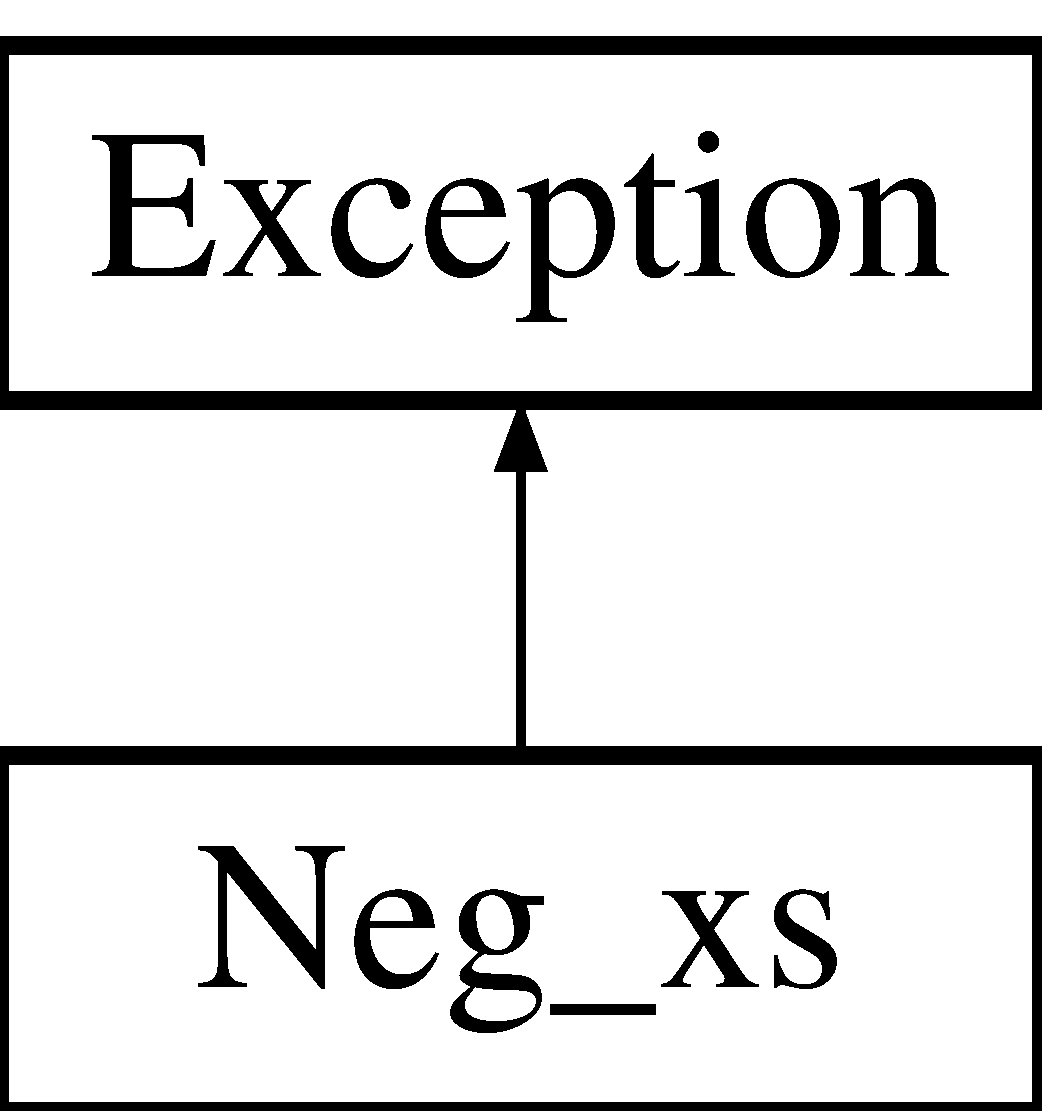
\includegraphics[height=2.000000cm]{classopenbu_1_1passlist_1_1_neg__xs}
\end{center}
\end{figure}


\doxysubsection{Detailed Description}
\begin{DoxyVerb}Raise when a negative cross-section is found\end{DoxyVerb}
 

The documentation for this class was generated from the following file\+:\begin{DoxyCompactItemize}
\item 
passlist.\+py\end{DoxyCompactItemize}

\hypertarget{classopenbu_1_1passport_1_1_no__fission___x_s}{}\section{No\+\_\+fission\+\_\+\+XS Class Reference}
\label{classopenbu_1_1passport_1_1_no__fission___x_s}\index{No\+\_\+fission\+\_\+\+XS@{No\+\_\+fission\+\_\+\+XS}}
Inheritance diagram for No\+\_\+fission\+\_\+\+XS\+:\begin{figure}[H]
\begin{center}
\leavevmode
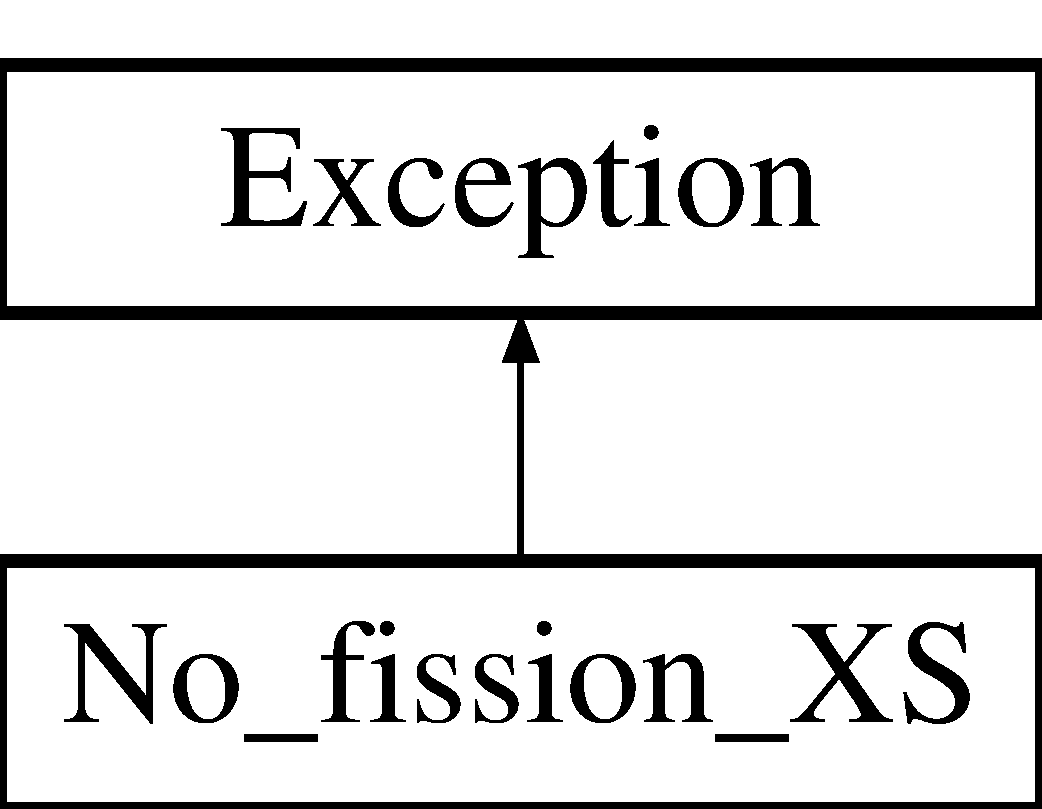
\includegraphics[height=2.000000cm]{classopenbu_1_1passport_1_1_no__fission___x_s}
\end{center}
\end{figure}


\subsection{Detailed Description}
\begin{DoxyVerb}Raise when the user tries to access fission XS for a nuclide which fission XS have not been set yet \end{DoxyVerb}
 

The documentation for this class was generated from the following file\+:\begin{DoxyCompactItemize}
\item 
/\+Users/mouginot/work/app/\+Open\+B\+U/openbu/\mbox{\hyperlink{passport_8py}{passport.\+py}}\end{DoxyCompactItemize}

\hypertarget{classopenbu_1_1passport_1_1_not__a___fission___product}{}\doxysection{Not\+\_\+a\+\_\+\+Fission\+\_\+\+Product Class Reference}
\label{classopenbu_1_1passport_1_1_not__a___fission___product}\index{Not\_a\_Fission\_Product@{Not\_a\_Fission\_Product}}
Inheritance diagram for Not\+\_\+a\+\_\+\+Fission\+\_\+\+Product\+:\begin{figure}[H]
\begin{center}
\leavevmode
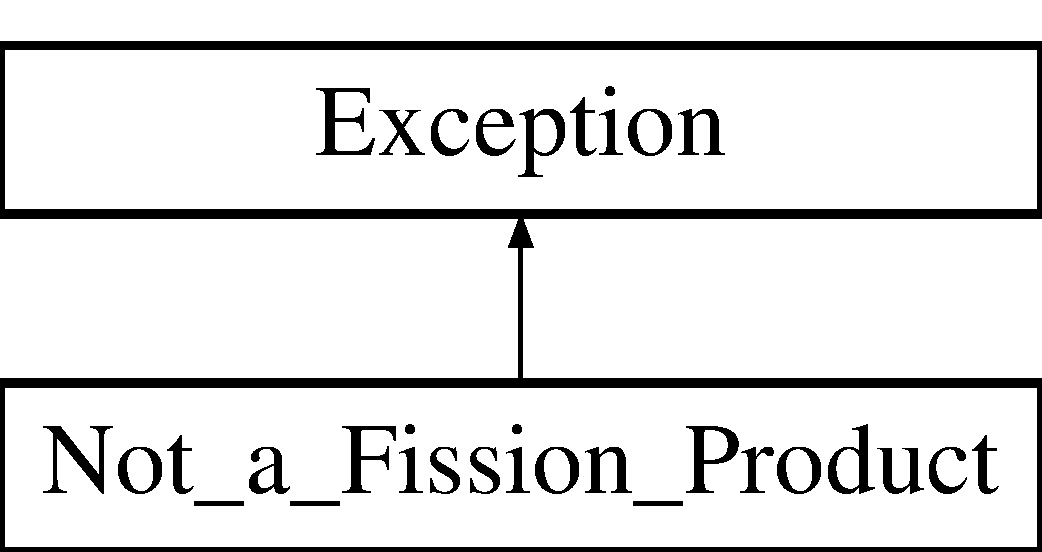
\includegraphics[height=2.000000cm]{classopenbu_1_1passport_1_1_not__a___fission___product}
\end{center}
\end{figure}


\doxysubsection{Detailed Description}
\begin{DoxyVerb}Raise when the user tries to set fission yields for a non fission product nuclide \end{DoxyVerb}
 

The documentation for this class was generated from the following file\+:\begin{DoxyCompactItemize}
\item 
passport.\+py\end{DoxyCompactItemize}

\hypertarget{classopenbu_1_1passport_1_1_nuc__xs__not__found}{}\section{Nuc\+\_\+xs\+\_\+not\+\_\+found Class Reference}
\label{classopenbu_1_1passport_1_1_nuc__xs__not__found}\index{Nuc\+\_\+xs\+\_\+not\+\_\+found@{Nuc\+\_\+xs\+\_\+not\+\_\+found}}
Inheritance diagram for Nuc\+\_\+xs\+\_\+not\+\_\+found\+:\begin{figure}[H]
\begin{center}
\leavevmode
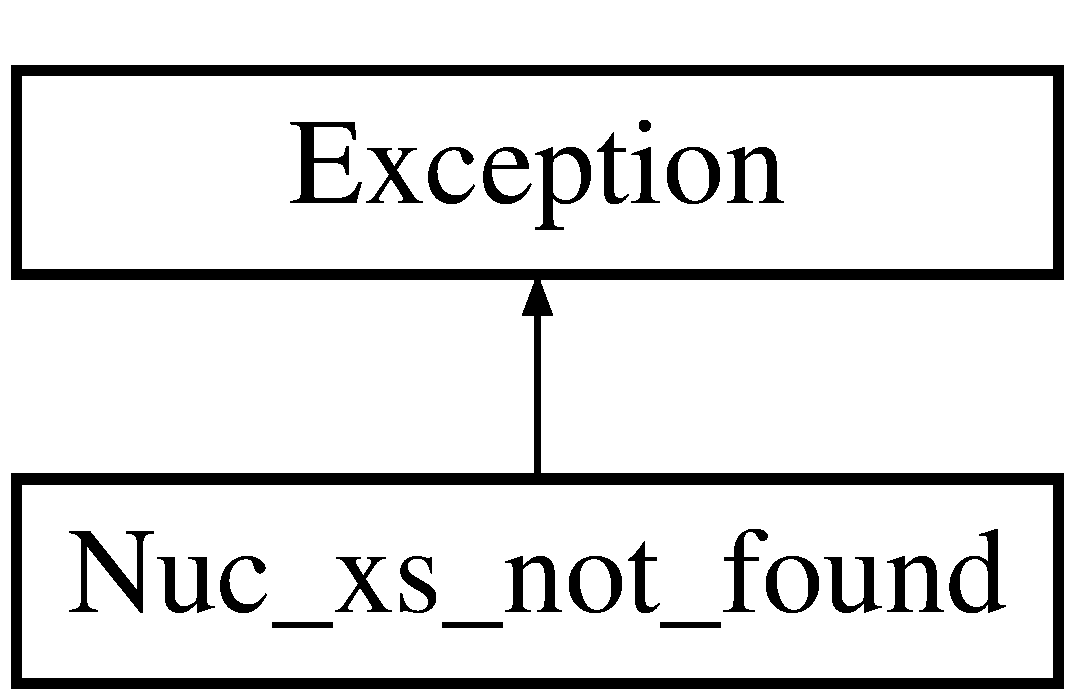
\includegraphics[height=2.000000cm]{classopenbu_1_1passport_1_1_nuc__xs__not__found}
\end{center}
\end{figure}


\subsection{Detailed Description}
\begin{DoxyVerb}Raise when the user requests a cross-sections of a nuclide that is not in the nuclide set \end{DoxyVerb}
 

The documentation for this class was generated from the following file\+:\begin{DoxyCompactItemize}
\item 
/\+Users/mouginot/work/app/\+Open\+B\+U/openbu/\mbox{\hyperlink{passport_8py}{passport.\+py}}\end{DoxyCompactItemize}

\hypertarget{classopenbu_1_1passlist_1_1_nuc__xs__not__found}{}\section{Nuc\+\_\+xs\+\_\+not\+\_\+found Class Reference}
\label{classopenbu_1_1passlist_1_1_nuc__xs__not__found}\index{Nuc\+\_\+xs\+\_\+not\+\_\+found@{Nuc\+\_\+xs\+\_\+not\+\_\+found}}
Inheritance diagram for Nuc\+\_\+xs\+\_\+not\+\_\+found\+:\begin{figure}[H]
\begin{center}
\leavevmode
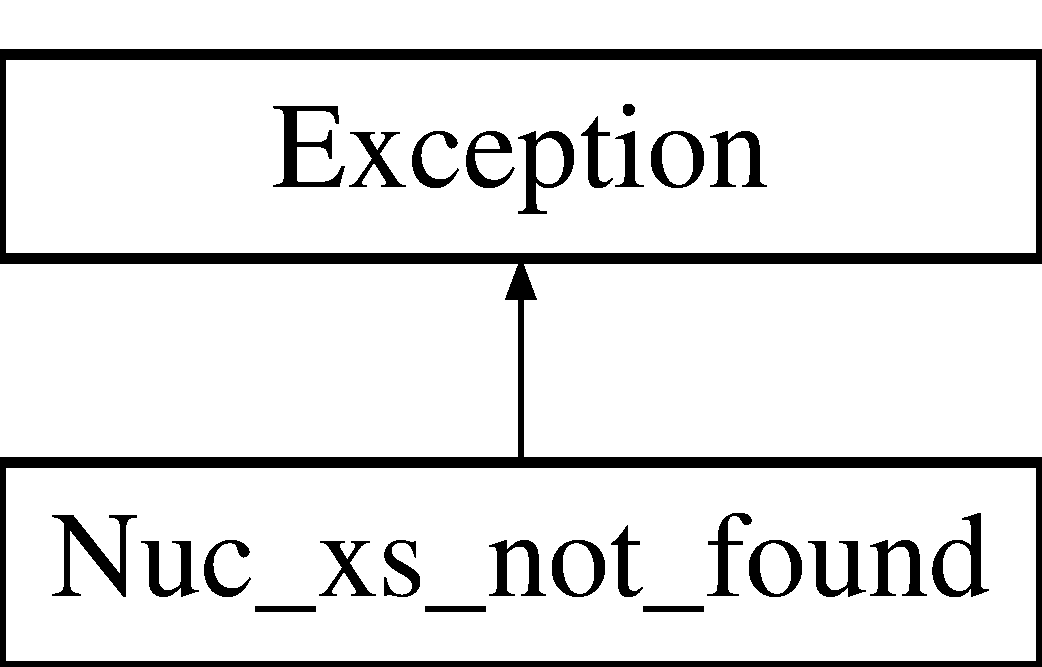
\includegraphics[height=2.000000cm]{classopenbu_1_1passlist_1_1_nuc__xs__not__found}
\end{center}
\end{figure}


\subsection{Detailed Description}
\begin{DoxyVerb}Raise when the user requests a cross-sections of a nuclide that is not in the nuclide set \end{DoxyVerb}
 

The documentation for this class was generated from the following file\+:\begin{DoxyCompactItemize}
\item 
/\+Users/mouginot/work/app/\+Open\+B\+U/openbu/\mbox{\hyperlink{passlist_8py}{passlist.\+py}}\end{DoxyCompactItemize}

\hypertarget{classopenbu_1_1cell_1_1_nucl__set__not__in___lib__nucl}{}\section{Nucl\+\_\+set\+\_\+not\+\_\+in\+\_\+\+Lib\+\_\+nucl Class Reference}
\label{classopenbu_1_1cell_1_1_nucl__set__not__in___lib__nucl}\index{Nucl\+\_\+set\+\_\+not\+\_\+in\+\_\+\+Lib\+\_\+nucl@{Nucl\+\_\+set\+\_\+not\+\_\+in\+\_\+\+Lib\+\_\+nucl}}
Inheritance diagram for Nucl\+\_\+set\+\_\+not\+\_\+in\+\_\+\+Lib\+\_\+nucl\+:\begin{figure}[H]
\begin{center}
\leavevmode
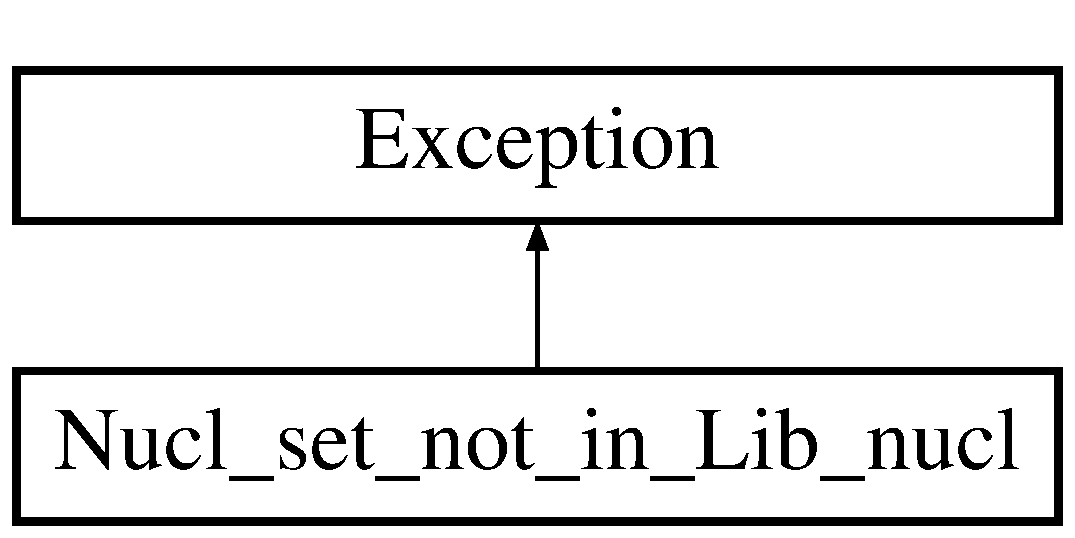
\includegraphics[height=2.000000cm]{classopenbu_1_1cell_1_1_nucl__set__not__in___lib__nucl}
\end{center}
\end{figure}


\subsection{Detailed Description}
\begin{DoxyVerb}Raise when the user forgot to set the initial nuclide of the cell and tries to burn cell\end{DoxyVerb}
 

The documentation for this class was generated from the following file\+:\begin{DoxyCompactItemize}
\item 
/\+Users/mouginot/work/app/\+Open\+B\+U/openbu/cell.\+py\end{DoxyCompactItemize}

\hypertarget{classopenbu_1_1cell_1_1_nuclide__list__redundant}{}\section{Nuclide\+\_\+list\+\_\+redundant Class Reference}
\label{classopenbu_1_1cell_1_1_nuclide__list__redundant}\index{Nuclide\+\_\+list\+\_\+redundant@{Nuclide\+\_\+list\+\_\+redundant}}
Inheritance diagram for Nuclide\+\_\+list\+\_\+redundant\+:\begin{figure}[H]
\begin{center}
\leavevmode
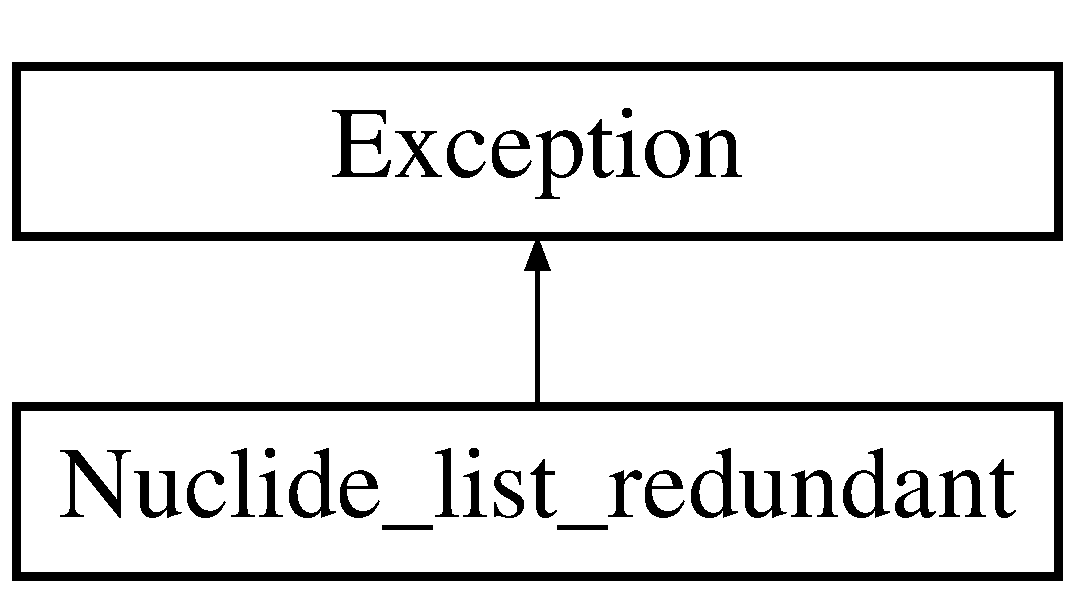
\includegraphics[height=2.000000cm]{classopenbu_1_1cell_1_1_nuclide__list__redundant}
\end{center}
\end{figure}


The documentation for this class was generated from the following file\+:\begin{DoxyCompactItemize}
\item 
/\+Users/mouginot/work/app/\+Open\+B\+U/openbu/\mbox{\hyperlink{cell_8py}{cell.\+py}}\end{DoxyCompactItemize}

\hypertarget{classopenbu_1_1passlist_1_1_passlist}{}\doxysection{Passlist Class Reference}
\label{classopenbu_1_1passlist_1_1_passlist}\index{Passlist@{Passlist}}
Inheritance diagram for Passlist\+:\begin{figure}[H]
\begin{center}
\leavevmode
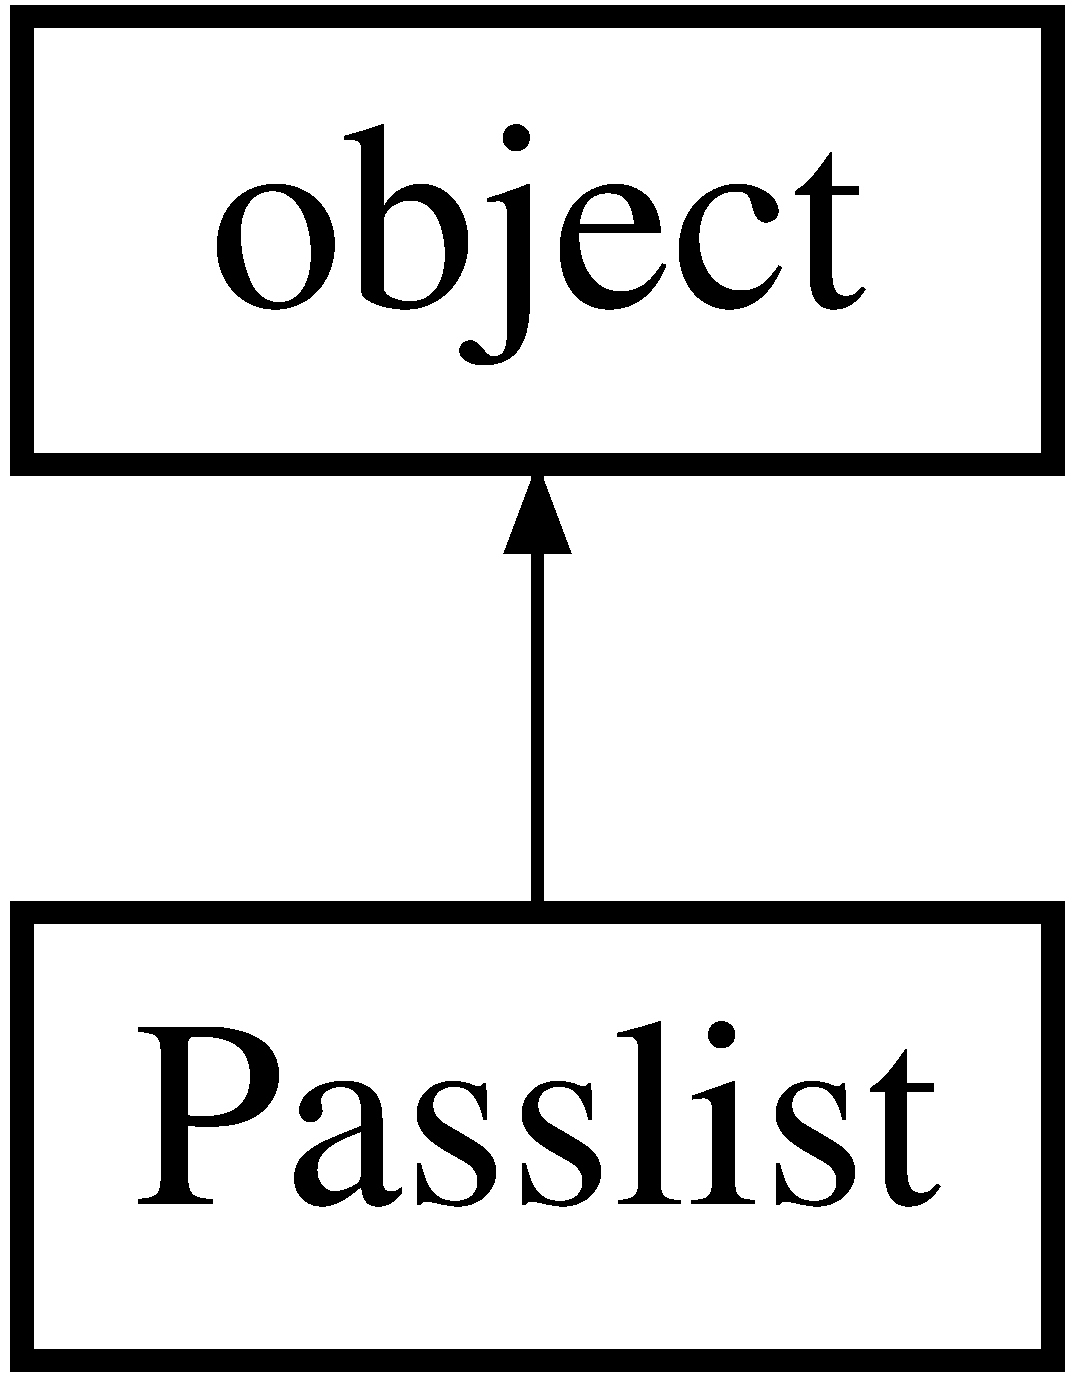
\includegraphics[height=2.000000cm]{classopenbu_1_1passlist_1_1_passlist}
\end{center}
\end{figure}
\doxysubsection*{Public Member Functions}
\doxysubsection*{Private Member Functions}
\doxysubsection*{Private Attributes}


\doxysubsection{Member Function Documentation}
\mbox{\Hypertarget{classopenbu_1_1passlist_1_1_passlist_a8c7ed2f12d3dbb3dd307013850e75afd}\label{classopenbu_1_1passlist_1_1_passlist_a8c7ed2f12d3dbb3dd307013850e75afd}} 
\index{Passlist@{Passlist}!\_get\_name\_passport\_dict@{\_get\_name\_passport\_dict}}
\index{\_get\_name\_passport\_dict@{\_get\_name\_passport\_dict}!Passlist@{Passlist}}
\doxysubsubsection{\texorpdfstring{\_get\_name\_passport\_dict()}{\_get\_name\_passport\_dict()}}
{\footnotesize\ttfamily def \+\_\+get\+\_\+name\+\_\+passport\+\_\+dict (\begin{DoxyParamCaption}\item[{}]{self }\end{DoxyParamCaption})\hspace{0.3cm}{\ttfamily [private]}}

\begin{DoxyVerb}Convert the list of passport into a dictionnary of passports where entries are the zamid of the nuclides\end{DoxyVerb}
 \mbox{\Hypertarget{classopenbu_1_1passlist_1_1_passlist_ac9b957ad1a1f7a2afccc7c7223110387}\label{classopenbu_1_1passlist_1_1_passlist_ac9b957ad1a1f7a2afccc7c7223110387}} 
\index{Passlist@{Passlist}!\_get\_zamid\_passport\_dict@{\_get\_zamid\_passport\_dict}}
\index{\_get\_zamid\_passport\_dict@{\_get\_zamid\_passport\_dict}!Passlist@{Passlist}}
\doxysubsubsection{\texorpdfstring{\_get\_zamid\_passport\_dict()}{\_get\_zamid\_passport\_dict()}}
{\footnotesize\ttfamily def \+\_\+get\+\_\+zamid\+\_\+passport\+\_\+dict (\begin{DoxyParamCaption}\item[{}]{self }\end{DoxyParamCaption})\hspace{0.3cm}{\ttfamily [private]}}

\begin{DoxyVerb}Convert the list of passport into a dictionnary of passports where entries are the zamid of the nuclides\end{DoxyVerb}
 \mbox{\Hypertarget{classopenbu_1_1passlist_1_1_passlist_a2eec6817afb9bc29c4c86d97cdb56947}\label{classopenbu_1_1passlist_1_1_passlist_a2eec6817afb9bc29c4c86d97cdb56947}} 
\index{Passlist@{Passlist}!\_overwrite\_xs@{\_overwrite\_xs}}
\index{\_overwrite\_xs@{\_overwrite\_xs}!Passlist@{Passlist}}
\doxysubsubsection{\texorpdfstring{\_overwrite\_xs()}{\_overwrite\_xs()}}
{\footnotesize\ttfamily def \+\_\+overwrite\+\_\+xs (\begin{DoxyParamCaption}\item[{}]{self,  }\item[{}]{xs\+\_\+dict }\end{DoxyParamCaption})\hspace{0.3cm}{\ttfamily [private]}}

\begin{DoxyVerb}Read and set the cross sections for each nuclide in the passports list\end{DoxyVerb}
 \mbox{\Hypertarget{classopenbu_1_1passlist_1_1_passlist_a4bf49923534fe53d939d4face28cf0f0}\label{classopenbu_1_1passlist_1_1_passlist_a4bf49923534fe53d939d4face28cf0f0}} 
\index{Passlist@{Passlist}!\_set\_decay@{\_set\_decay}}
\index{\_set\_decay@{\_set\_decay}!Passlist@{Passlist}}
\doxysubsubsection{\texorpdfstring{\_set\_decay()}{\_set\_decay()}}
{\footnotesize\ttfamily def \+\_\+set\+\_\+decay (\begin{DoxyParamCaption}\item[{}]{self,  }\item[{}]{decay\+\_\+lib\+\_\+b,  }\item[{}]{decay\+\_\+lib\+\_\+a }\end{DoxyParamCaption})\hspace{0.3cm}{\ttfamily [private]}}

\begin{DoxyVerb}Read and set the decay constants for each nuclide in the passports list\end{DoxyVerb}
 \mbox{\Hypertarget{classopenbu_1_1passlist_1_1_passlist_a29902b392d57e73485c65bfbfdff566e}\label{classopenbu_1_1passlist_1_1_passlist_a29902b392d57e73485c65bfbfdff566e}} 
\index{Passlist@{Passlist}!\_set\_fy@{\_set\_fy}}
\index{\_set\_fy@{\_set\_fy}!Passlist@{Passlist}}
\doxysubsubsection{\texorpdfstring{\_set\_fy()}{\_set\_fy()}}
{\footnotesize\ttfamily def \+\_\+set\+\_\+fy (\begin{DoxyParamCaption}\item[{}]{self,  }\item[{}]{fy\+\_\+dict }\end{DoxyParamCaption})\hspace{0.3cm}{\ttfamily [private]}}

\begin{DoxyVerb}Read and set the fission yields for fission products in the passports list\end{DoxyVerb}
 \mbox{\Hypertarget{classopenbu_1_1passlist_1_1_passlist_a956fb79a1bafe4c9a4f831ed4be4005c}\label{classopenbu_1_1passlist_1_1_passlist_a956fb79a1bafe4c9a4f831ed4be4005c}} 
\index{Passlist@{Passlist}!\_set\_mass@{\_set\_mass}}
\index{\_set\_mass@{\_set\_mass}!Passlist@{Passlist}}
\doxysubsubsection{\texorpdfstring{\_set\_mass()}{\_set\_mass()}}
{\footnotesize\ttfamily def \+\_\+set\+\_\+mass (\begin{DoxyParamCaption}\item[{}]{self,  }\item[{}]{passport\+\_\+list }\end{DoxyParamCaption})\hspace{0.3cm}{\ttfamily [private]}}

\begin{DoxyVerb}Read and set the atomic mass for each nuclide in the passports list\end{DoxyVerb}
 \mbox{\Hypertarget{classopenbu_1_1passlist_1_1_passlist_aa45dff0e552a6f90aef82cfd5c0691b9}\label{classopenbu_1_1passlist_1_1_passlist_aa45dff0e552a6f90aef82cfd5c0691b9}} 
\index{Passlist@{Passlist}!\_set\_xs@{\_set\_xs}}
\index{\_set\_xs@{\_set\_xs}!Passlist@{Passlist}}
\doxysubsubsection{\texorpdfstring{\_set\_xs()}{\_set\_xs()}}
{\footnotesize\ttfamily def \+\_\+set\+\_\+xs (\begin{DoxyParamCaption}\item[{}]{self,  }\item[{}]{xs\+\_\+dict }\end{DoxyParamCaption})\hspace{0.3cm}{\ttfamily [private]}}

\begin{DoxyVerb}Read and set the cross sections for each nuclide in the passports list\end{DoxyVerb}
 

The documentation for this class was generated from the following file\+:\begin{DoxyCompactItemize}
\item 
passlist.\+py\end{DoxyCompactItemize}

\hypertarget{classopenbu_1_1cell_1_1_passlist__not__defined}{}\section{Passlist\+\_\+not\+\_\+defined Class Reference}
\label{classopenbu_1_1cell_1_1_passlist__not__defined}\index{Passlist\+\_\+not\+\_\+defined@{Passlist\+\_\+not\+\_\+defined}}
Inheritance diagram for Passlist\+\_\+not\+\_\+defined\+:\begin{figure}[H]
\begin{center}
\leavevmode
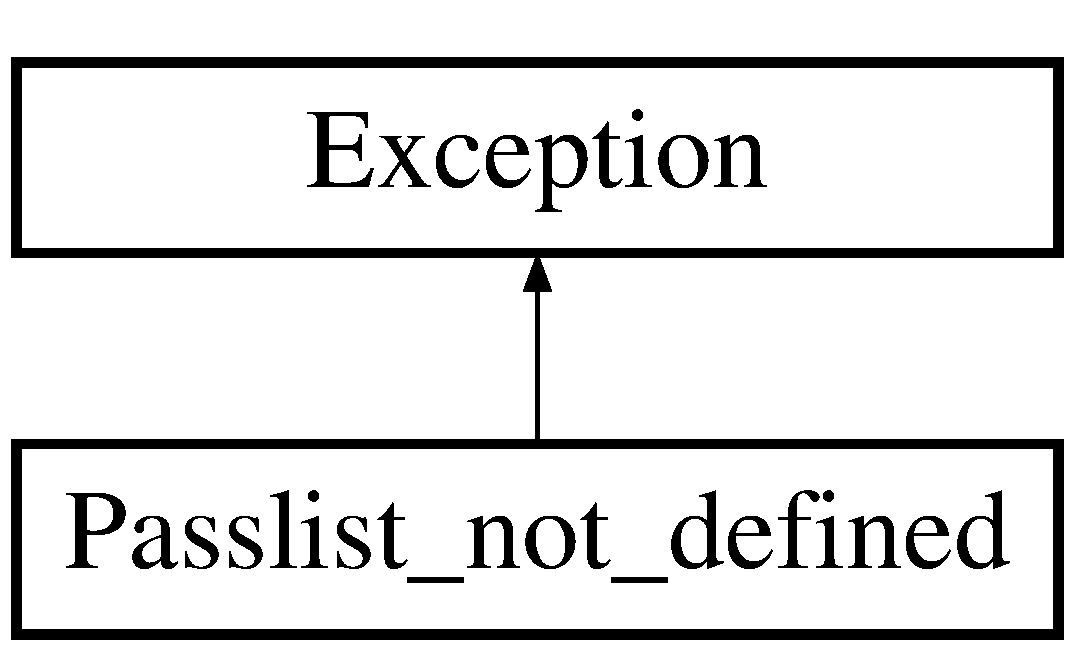
\includegraphics[height=2.000000cm]{classopenbu_1_1cell_1_1_passlist__not__defined}
\end{center}
\end{figure}


\subsection{Detailed Description}
\begin{DoxyVerb}Raise when the user forgot to defined passlist for a cell\end{DoxyVerb}
 

The documentation for this class was generated from the following file\+:\begin{DoxyCompactItemize}
\item 
/\+Users/mouginot/work/app/\+Open\+B\+U/openbu/cell.\+py\end{DoxyCompactItemize}

\hypertarget{classopenbu_1_1passport_1_1_passport}{}\doxysection{Passport Class Reference}
\label{classopenbu_1_1passport_1_1_passport}\index{Passport@{Passport}}
Inheritance diagram for Passport\+:\begin{figure}[H]
\begin{center}
\leavevmode
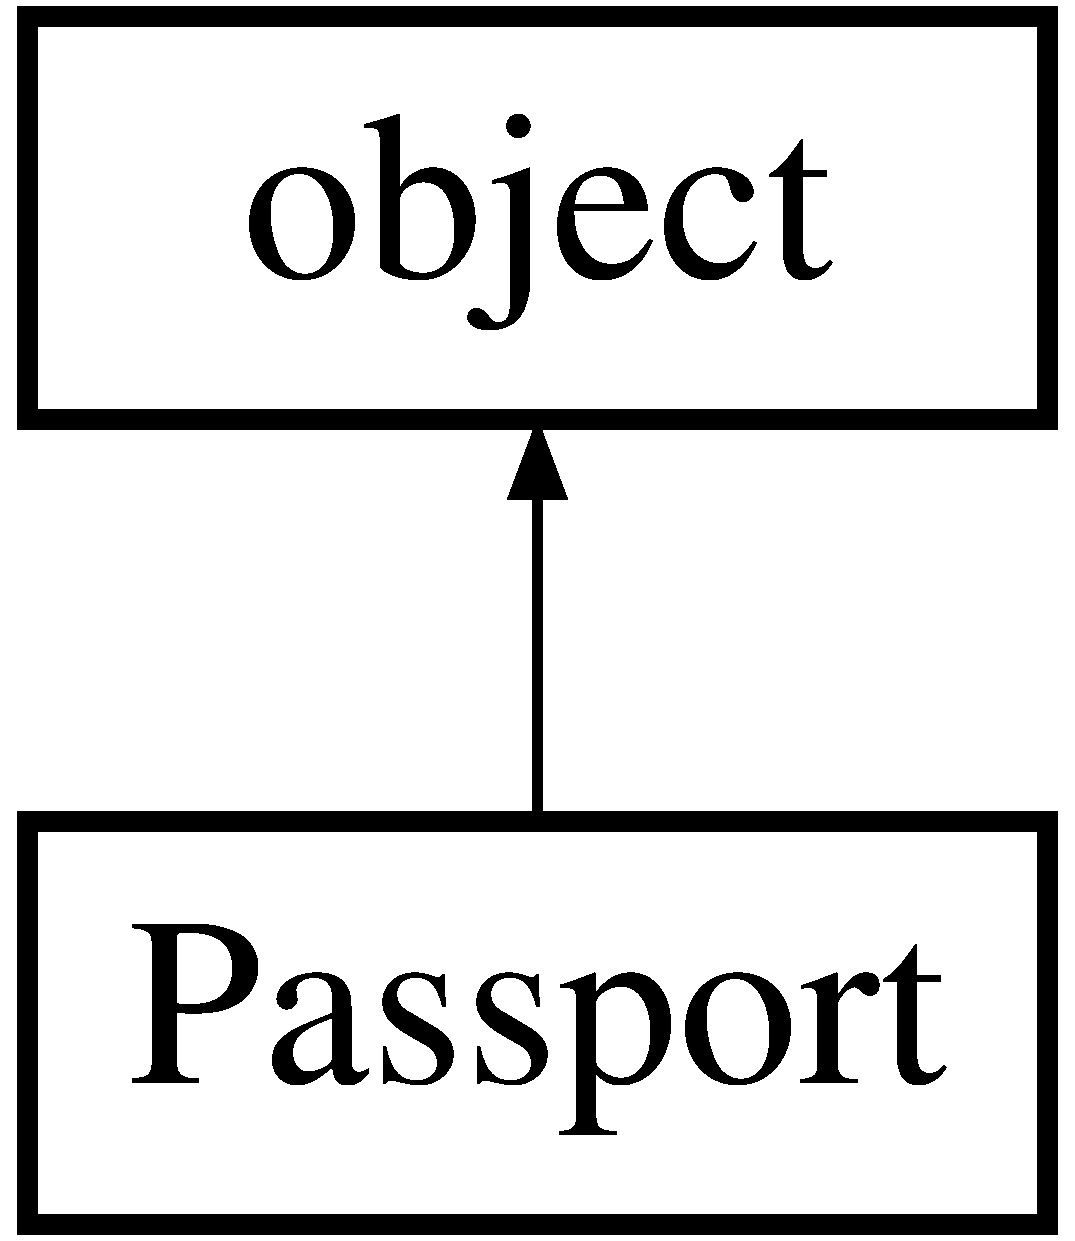
\includegraphics[height=2.000000cm]{classopenbu_1_1passport_1_1_passport}
\end{center}
\end{figure}
\doxysubsection*{Public Member Functions}
\doxysubsection*{Public Attributes}
\doxysubsection*{Private Member Functions}
\doxysubsection*{Private Attributes}
\doxysubsection*{Static Private Attributes}


\doxysubsection{Detailed Description}
\begin{DoxyVerb}passport stores all the relevant data of indivudual nuclides and offers methods to extract information on them

   The passport class is individually instantiated for each nuclide. It contains two types of information: constant and variable data.
   Constant data, such as the atomic mass, decay constant or the element's family (actinide, fission product) do not change over the course of a simulation.
   Variable data such as cross sections or fission yields do vary during a simulation and need thus to be updated regularly during a simulation.
   Some of the data are created at the time of the instantiation of the class for a nuclide such as the element's family or the nuclide's
   neutron reaction daughters. Other type of data, typically large in size such as cross sections and decay constants, are to be explicitly set or loaded.
   A setter method will enable any script that reads the data source to set this data for the passport of a specific nuclide. This is the method used within
   the code of Open-Burnup to set the data for a list of passports. The other way to explicitly set the data is to use the loader method. This method will
   go to the data source itself, read the data and set it for the passport of a specific nuclide. This method is envision to be used by the user as a
   user-friendly way to get information on individual nuclides.

   Attributes:
       * **decay_a:** returns the absolute value of the decay constants of the nuclide
       * **decay_b:** returns the percent fraction value of the decay constants of the nuclide
       * **fy:** returns the value of fission yields in percent
       * **mass:** returns the atomic mass of the nuclide
       * **xs:** returns the absolute value of cross sections for the nuclide
       * **FAM:** returns the family group name of the nuclide
       * **xs_relatives:** returns neutron reaction's daughter nuclides' id
       * **decay_relatives:** returns decay reaction's daughter nuclides' id

   Methods:
       * **set_mass():** set the atomic mass of the nuclide
       * **set_decay():** set the decay constants (both absolute values and percent fractions) of the nuclide
       * **set_xs():** set the cross sections of the nuclide
       * **set_fy():** set the fission yields of the nuclide
       * **load_mass():** load the atomic mass of the nuclide
       * **load_decay():** load the decay constants (both absolute values and percent fractions) of the nuclide
       * **load_mass():** load the cross sections of the nuclide
       * **load_mass():** load the fission yields of the nuclide
       * **get__zamid():** returns the zzaaam id of the nuclide
       * **get_nuc_name():** returns the name of the nuclide\end{DoxyVerb}
 

\doxysubsection{Member Function Documentation}
\mbox{\Hypertarget{classopenbu_1_1passport_1_1_passport_a1d13e38c1df92265a6b65961522978e9}\label{classopenbu_1_1passport_1_1_passport_a1d13e38c1df92265a6b65961522978e9}} 
\index{Passport@{Passport}!\_set\_initial\_dens@{\_set\_initial\_dens}}
\index{\_set\_initial\_dens@{\_set\_initial\_dens}!Passport@{Passport}}
\doxysubsubsection{\texorpdfstring{\_set\_initial\_dens()}{\_set\_initial\_dens()}}
{\footnotesize\ttfamily def \+\_\+set\+\_\+initial\+\_\+dens (\begin{DoxyParamCaption}\item[{}]{self,  }\item[{}]{new\+\_\+dens }\end{DoxyParamCaption})\hspace{0.3cm}{\ttfamily [private]}}

\begin{DoxyVerb}set new dens to current dens and append to dens_seqor\end{DoxyVerb}
 \mbox{\Hypertarget{classopenbu_1_1passport_1_1_passport_a3f7ead3ec8497f2dea2c5b4a8efb3064}\label{classopenbu_1_1passport_1_1_passport_a3f7ead3ec8497f2dea2c5b4a8efb3064}} 
\index{Passport@{Passport}!\_set\_state@{\_set\_state}}
\index{\_set\_state@{\_set\_state}!Passport@{Passport}}
\doxysubsubsection{\texorpdfstring{\_set\_state()}{\_set\_state()}}
{\footnotesize\ttfamily def \+\_\+set\+\_\+state (\begin{DoxyParamCaption}\item[{}]{self }\end{DoxyParamCaption})\hspace{0.3cm}{\ttfamily [private]}}

\begin{DoxyVerb}Returns the state of the nuclide (excited or ground state)\end{DoxyVerb}
 \mbox{\Hypertarget{classopenbu_1_1passport_1_1_passport_aae6f90e1f0871cddaad54d66a6bd6529}\label{classopenbu_1_1passport_1_1_passport_aae6f90e1f0871cddaad54d66a6bd6529}} 
\index{Passport@{Passport}!current\_dens@{current\_dens}}
\index{current\_dens@{current\_dens}!Passport@{Passport}}
\doxysubsubsection{\texorpdfstring{current\_dens()}{current\_dens()}\hspace{0.1cm}{\footnotesize\ttfamily [1/2]}}
{\footnotesize\ttfamily def current\+\_\+dens (\begin{DoxyParamCaption}\item[{}]{self }\end{DoxyParamCaption})}

\begin{DoxyVerb}Returns the density of the nuclide in atom per cm^3\end{DoxyVerb}
 \mbox{\Hypertarget{classopenbu_1_1passport_1_1_passport_a2e640e060087e64c0e938f17b6c3653e}\label{classopenbu_1_1passport_1_1_passport_a2e640e060087e64c0e938f17b6c3653e}} 
\index{Passport@{Passport}!current\_dens@{current\_dens}}
\index{current\_dens@{current\_dens}!Passport@{Passport}}
\doxysubsubsection{\texorpdfstring{current\_dens()}{current\_dens()}\hspace{0.1cm}{\footnotesize\ttfamily [2/2]}}
{\footnotesize\ttfamily def current\+\_\+dens (\begin{DoxyParamCaption}\item[{}]{self,  }\item[{}]{new\+\_\+dens }\end{DoxyParamCaption})}

\begin{DoxyVerb}set the density of the nuclide in atom per cm^3\end{DoxyVerb}
 \mbox{\Hypertarget{classopenbu_1_1passport_1_1_passport_a555c209d9b1ea0fcc30cb14a259342f4}\label{classopenbu_1_1passport_1_1_passport_a555c209d9b1ea0fcc30cb14a259342f4}} 
\index{Passport@{Passport}!current\_xs@{current\_xs}}
\index{current\_xs@{current\_xs}!Passport@{Passport}}
\doxysubsubsection{\texorpdfstring{current\_xs()}{current\_xs()}}
{\footnotesize\ttfamily def current\+\_\+xs (\begin{DoxyParamCaption}\item[{}]{self }\end{DoxyParamCaption})}

\begin{DoxyVerb}Returns the cross sections data of the nuclide\end{DoxyVerb}
 \mbox{\Hypertarget{classopenbu_1_1passport_1_1_passport_ab9d903431dc1a815d57cb09912e41e58}\label{classopenbu_1_1passport_1_1_passport_ab9d903431dc1a815d57cb09912e41e58}} 
\index{Passport@{Passport}!decay\_a@{decay\_a}}
\index{decay\_a@{decay\_a}!Passport@{Passport}}
\doxysubsubsection{\texorpdfstring{decay\_a()}{decay\_a()}}
{\footnotesize\ttfamily def decay\+\_\+a (\begin{DoxyParamCaption}\item[{}]{self }\end{DoxyParamCaption})}

\begin{DoxyVerb}Returns the absolute values of the decay constant of the nuclide\end{DoxyVerb}
 \mbox{\Hypertarget{classopenbu_1_1passport_1_1_passport_ade7165602b6bcdee1ed9b7256170379b}\label{classopenbu_1_1passport_1_1_passport_ade7165602b6bcdee1ed9b7256170379b}} 
\index{Passport@{Passport}!decay\_b@{decay\_b}}
\index{decay\_b@{decay\_b}!Passport@{Passport}}
\doxysubsubsection{\texorpdfstring{decay\_b()}{decay\_b()}}
{\footnotesize\ttfamily def decay\+\_\+b (\begin{DoxyParamCaption}\item[{}]{self }\end{DoxyParamCaption})}

\begin{DoxyVerb}Returns the fraction percent values of the decay constant of the nuclide\end{DoxyVerb}
 \mbox{\Hypertarget{classopenbu_1_1passport_1_1_passport_afe7a50b1cfeb99651932d201b32e1eac}\label{classopenbu_1_1passport_1_1_passport_afe7a50b1cfeb99651932d201b32e1eac}} 
\index{Passport@{Passport}!decay\_child@{decay\_child}}
\index{decay\_child@{decay\_child}!Passport@{Passport}}
\doxysubsubsection{\texorpdfstring{decay\_child()}{decay\_child()}}
{\footnotesize\ttfamily def decay\+\_\+child (\begin{DoxyParamCaption}\item[{}]{self }\end{DoxyParamCaption})}

\begin{DoxyVerb}Returns the decay reactions' daughter products\end{DoxyVerb}
 \mbox{\Hypertarget{classopenbu_1_1passport_1_1_passport_a036610ac850c29ffb1e5172cff7c679a}\label{classopenbu_1_1passport_1_1_passport_a036610ac850c29ffb1e5172cff7c679a}} 
\index{Passport@{Passport}!decay\_parent@{decay\_parent}}
\index{decay\_parent@{decay\_parent}!Passport@{Passport}}
\doxysubsubsection{\texorpdfstring{decay\_parent()}{decay\_parent()}}
{\footnotesize\ttfamily def decay\+\_\+parent (\begin{DoxyParamCaption}\item[{}]{self }\end{DoxyParamCaption})}

\begin{DoxyVerb}Returns the decay reactions' daughter products\end{DoxyVerb}
 \mbox{\Hypertarget{classopenbu_1_1passport_1_1_passport_a8b75ace3008810461600cc7df511303b}\label{classopenbu_1_1passport_1_1_passport_a8b75ace3008810461600cc7df511303b}} 
\index{Passport@{Passport}!fy@{fy}}
\index{fy@{fy}!Passport@{Passport}}
\doxysubsubsection{\texorpdfstring{fy()}{fy()}}
{\footnotesize\ttfamily def fy (\begin{DoxyParamCaption}\item[{}]{self }\end{DoxyParamCaption})}

\begin{DoxyVerb}Returns the fission yields data in percent\end{DoxyVerb}
 \mbox{\Hypertarget{classopenbu_1_1passport_1_1_passport_aa1146a83b02f1768536bf28e3f5776ea}\label{classopenbu_1_1passport_1_1_passport_aa1146a83b02f1768536bf28e3f5776ea}} 
\index{Passport@{Passport}!get\_a@{get\_a}}
\index{get\_a@{get\_a}!Passport@{Passport}}
\doxysubsubsection{\texorpdfstring{get\_a()}{get\_a()}}
{\footnotesize\ttfamily def get\+\_\+a (\begin{DoxyParamCaption}\item[{}]{self }\end{DoxyParamCaption})}

\begin{DoxyVerb}Returns the mass number of the nuclide\end{DoxyVerb}
 \mbox{\Hypertarget{classopenbu_1_1passport_1_1_passport_aa75b75b6a9d2a68e6a592e7353044edb}\label{classopenbu_1_1passport_1_1_passport_aa75b75b6a9d2a68e6a592e7353044edb}} 
\index{Passport@{Passport}!get\_z@{get\_z}}
\index{get\_z@{get\_z}!Passport@{Passport}}
\doxysubsubsection{\texorpdfstring{get\_z()}{get\_z()}}
{\footnotesize\ttfamily def get\+\_\+z (\begin{DoxyParamCaption}\item[{}]{self }\end{DoxyParamCaption})}

\begin{DoxyVerb}Returns the atomic number of the nuclide\end{DoxyVerb}
 \mbox{\Hypertarget{classopenbu_1_1passport_1_1_passport_ab6f7c3af79510d2bf012aa1a483a6cf8}\label{classopenbu_1_1passport_1_1_passport_ab6f7c3af79510d2bf012aa1a483a6cf8}} 
\index{Passport@{Passport}!load\_decay@{load\_decay}}
\index{load\_decay@{load\_decay}!Passport@{Passport}}
\doxysubsubsection{\texorpdfstring{load\_decay()}{load\_decay()}}
{\footnotesize\ttfamily def load\+\_\+decay (\begin{DoxyParamCaption}\item[{}]{self }\end{DoxyParamCaption})}

\begin{DoxyVerb}Load the decay constant value of the nuclide

This method directly fetches the decay constant values from the source data and automatically set
of the passport object\end{DoxyVerb}
 \mbox{\Hypertarget{classopenbu_1_1passport_1_1_passport_a3fd9b285c12428f2f1021f6fa498d27b}\label{classopenbu_1_1passport_1_1_passport_a3fd9b285c12428f2f1021f6fa498d27b}} 
\index{Passport@{Passport}!load\_fy@{load\_fy}}
\index{load\_fy@{load\_fy}!Passport@{Passport}}
\doxysubsubsection{\texorpdfstring{load\_fy()}{load\_fy()}}
{\footnotesize\ttfamily def load\+\_\+fy (\begin{DoxyParamCaption}\item[{}]{self }\end{DoxyParamCaption})}

\begin{DoxyVerb}Load the fission yields data of the nuclide

This method directly fetches the fission yields data from the source data and automatically set
of the passport object

If the nuclide for which the fission yields data are being loaded is not a fission product,
the error *Not_a_Fission_Product* will be raised\end{DoxyVerb}
 \mbox{\Hypertarget{classopenbu_1_1passport_1_1_passport_a791d705e172d19c0cdc181960287cc78}\label{classopenbu_1_1passport_1_1_passport_a791d705e172d19c0cdc181960287cc78}} 
\index{Passport@{Passport}!load\_mass@{load\_mass}}
\index{load\_mass@{load\_mass}!Passport@{Passport}}
\doxysubsubsection{\texorpdfstring{load\_mass()}{load\_mass()}}
{\footnotesize\ttfamily def load\+\_\+mass (\begin{DoxyParamCaption}\item[{}]{self }\end{DoxyParamCaption})}

\begin{DoxyVerb}Load the atomic mass of the nuclide in gram

This method directly fetches the atomic mass from the source data and automatically set
of the passport object\end{DoxyVerb}
 \mbox{\Hypertarget{classopenbu_1_1passport_1_1_passport_a1687aea883b9cdececdb7b88b659cd5c}\label{classopenbu_1_1passport_1_1_passport_a1687aea883b9cdececdb7b88b659cd5c}} 
\index{Passport@{Passport}!load\_xs@{load\_xs}}
\index{load\_xs@{load\_xs}!Passport@{Passport}}
\doxysubsubsection{\texorpdfstring{load\_xs()}{load\_xs()}}
{\footnotesize\ttfamily def load\+\_\+xs (\begin{DoxyParamCaption}\item[{}]{self }\end{DoxyParamCaption})}

\begin{DoxyVerb}Load the cross sections data of the nuclide

This method directly fetches the cross sections data from the source data and automatically set
of the passport object\end{DoxyVerb}
 \mbox{\Hypertarget{classopenbu_1_1passport_1_1_passport_a69ae279139576858c6ca4dc9f5912717}\label{classopenbu_1_1passport_1_1_passport_a69ae279139576858c6ca4dc9f5912717}} 
\index{Passport@{Passport}!mass@{mass}}
\index{mass@{mass}!Passport@{Passport}}
\doxysubsubsection{\texorpdfstring{mass()}{mass()}}
{\footnotesize\ttfamily def mass (\begin{DoxyParamCaption}\item[{}]{self }\end{DoxyParamCaption})}

\begin{DoxyVerb}Return the atomic mass of the nuclide in gram\end{DoxyVerb}
 \mbox{\Hypertarget{classopenbu_1_1passport_1_1_passport_ae04c67eded9e7f018b551d4be5d36f2c}\label{classopenbu_1_1passport_1_1_passport_ae04c67eded9e7f018b551d4be5d36f2c}} 
\index{Passport@{Passport}!set\_decay@{set\_decay}}
\index{set\_decay@{set\_decay}!Passport@{Passport}}
\doxysubsubsection{\texorpdfstring{set\_decay()}{set\_decay()}}
{\footnotesize\ttfamily def set\+\_\+decay (\begin{DoxyParamCaption}\item[{}]{self,  }\item[{}]{decay\+\_\+a,  }\item[{}]{decay\+\_\+b }\end{DoxyParamCaption})}

\begin{DoxyVerb}Set the absolute and fracional values of the decay constant of the nuclide\end{DoxyVerb}
 \mbox{\Hypertarget{classopenbu_1_1passport_1_1_passport_af0b4eabf69455a1ace31fadfc437695b}\label{classopenbu_1_1passport_1_1_passport_af0b4eabf69455a1ace31fadfc437695b}} 
\index{Passport@{Passport}!xs\_child@{xs\_child}}
\index{xs\_child@{xs\_child}!Passport@{Passport}}
\doxysubsubsection{\texorpdfstring{xs\_child()}{xs\_child()}}
{\footnotesize\ttfamily def xs\+\_\+child (\begin{DoxyParamCaption}\item[{}]{self }\end{DoxyParamCaption})}

\begin{DoxyVerb}Returns the neutron reactions' daughter products\end{DoxyVerb}
 \mbox{\Hypertarget{classopenbu_1_1passport_1_1_passport_a0f25e060e526ebc2db82f4769504a0b4}\label{classopenbu_1_1passport_1_1_passport_a0f25e060e526ebc2db82f4769504a0b4}} 
\index{Passport@{Passport}!xs\_parent@{xs\_parent}}
\index{xs\_parent@{xs\_parent}!Passport@{Passport}}
\doxysubsubsection{\texorpdfstring{xs\_parent()}{xs\_parent()}}
{\footnotesize\ttfamily def xs\+\_\+parent (\begin{DoxyParamCaption}\item[{}]{self }\end{DoxyParamCaption})}

\begin{DoxyVerb}Returns the neutron reactions' daughter products\end{DoxyVerb}
 

The documentation for this class was generated from the following file\+:\begin{DoxyCompactItemize}
\item 
passport.\+py\end{DoxyCompactItemize}

\hypertarget{classopenbu_1_1sequence_1_1_sequence}{}\section{Sequence Class Reference}
\label{classopenbu_1_1sequence_1_1_sequence}\index{Sequence@{Sequence}}
Inheritance diagram for Sequence\+:\begin{figure}[H]
\begin{center}
\leavevmode
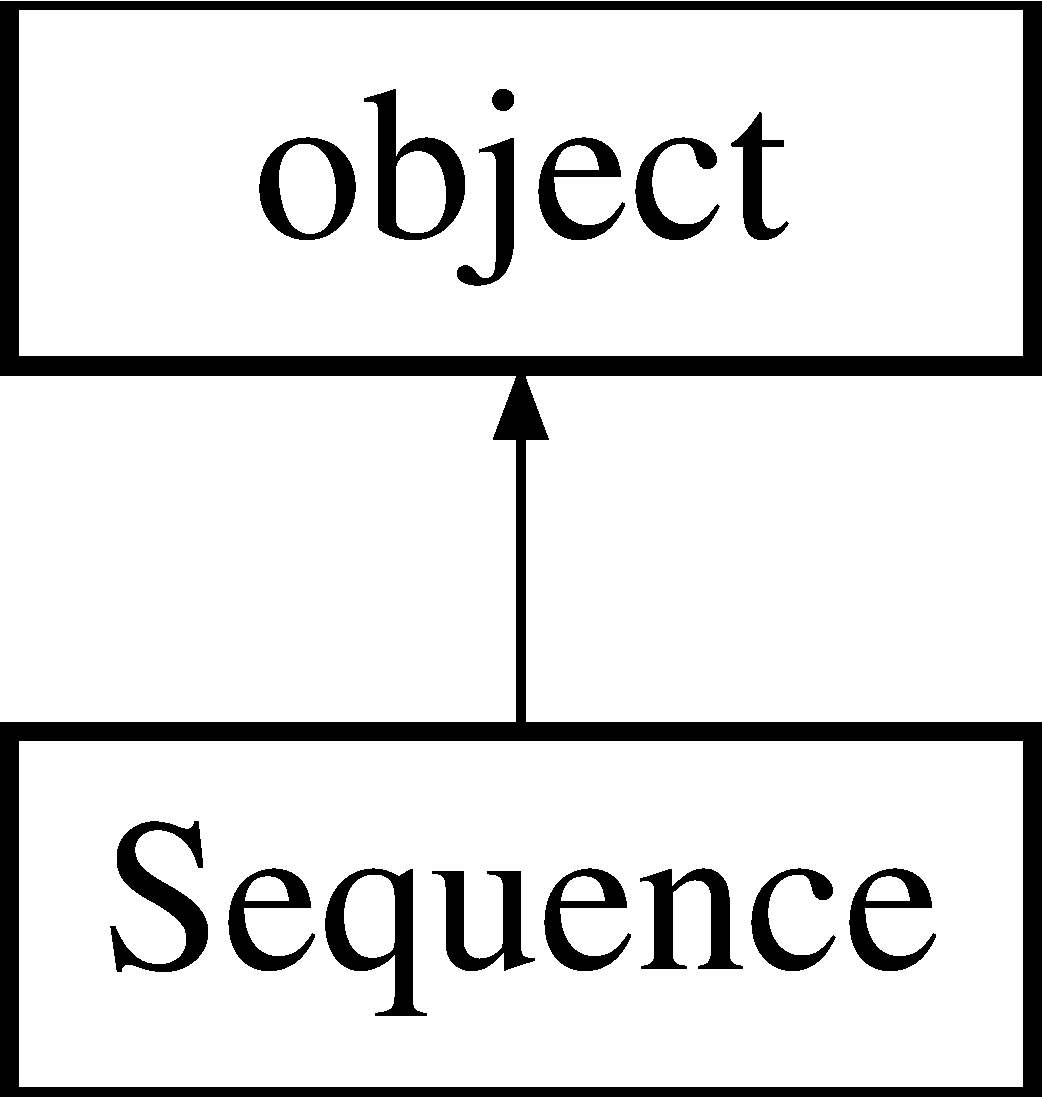
\includegraphics[height=2.000000cm]{classopenbu_1_1sequence_1_1_sequence}
\end{center}
\end{figure}
\subsection*{Public Member Functions}
\subsection*{Public Attributes}
\subsection*{Private Member Functions}
\subsection*{Private Attributes}


\subsection{Member Function Documentation}
\mbox{\Hypertarget{classopenbu_1_1sequence_1_1_sequence_aa4fed9a7ae1513bbb0db097c62569bd3}\label{classopenbu_1_1sequence_1_1_sequence_aa4fed9a7ae1513bbb0db097c62569bd3}} 
\index{openbu\+::sequence\+::\+Sequence@{openbu\+::sequence\+::\+Sequence}!\+\_\+set\+\_\+initial\+\_\+flux@{\+\_\+set\+\_\+initial\+\_\+flux}}
\index{\+\_\+set\+\_\+initial\+\_\+flux@{\+\_\+set\+\_\+initial\+\_\+flux}!openbu\+::sequence\+::\+Sequence@{openbu\+::sequence\+::\+Sequence}}
\subsubsection{\texorpdfstring{\+\_\+set\+\_\+initial\+\_\+flux()}{\_set\_initial\_flux()}}
{\footnotesize\ttfamily def \+\_\+set\+\_\+initial\+\_\+flux (\begin{DoxyParamCaption}\item[{}]{self,  }\item[{}]{new\+\_\+flux }\end{DoxyParamCaption})\hspace{0.3cm}{\ttfamily [private]}}

\begin{DoxyVerb}set new new_flux to current flux and append to flux sequence\end{DoxyVerb}
 \mbox{\Hypertarget{classopenbu_1_1sequence_1_1_sequence_a824e7bd80e4d7312e7327103b4862906}\label{classopenbu_1_1sequence_1_1_sequence_a824e7bd80e4d7312e7327103b4862906}} 
\index{openbu\+::sequence\+::\+Sequence@{openbu\+::sequence\+::\+Sequence}!\+\_\+set\+\_\+initial\+\_\+pow\+\_\+dens@{\+\_\+set\+\_\+initial\+\_\+pow\+\_\+dens}}
\index{\+\_\+set\+\_\+initial\+\_\+pow\+\_\+dens@{\+\_\+set\+\_\+initial\+\_\+pow\+\_\+dens}!openbu\+::sequence\+::\+Sequence@{openbu\+::sequence\+::\+Sequence}}
\subsubsection{\texorpdfstring{\+\_\+set\+\_\+initial\+\_\+pow\+\_\+dens()}{\_set\_initial\_pow\_dens()}}
{\footnotesize\ttfamily def \+\_\+set\+\_\+initial\+\_\+pow\+\_\+dens (\begin{DoxyParamCaption}\item[{}]{self,  }\item[{}]{new\+\_\+pow\+\_\+dens }\end{DoxyParamCaption})\hspace{0.3cm}{\ttfamily [private]}}

\begin{DoxyVerb}set new new_pow_dens to current pow_dens and append to pow_dens sequence\end{DoxyVerb}
 

The documentation for this class was generated from the following file\+:\begin{DoxyCompactItemize}
\item 
/\+Users/mouginot/work/app/\+Open\+B\+U/openbu/sequence.\+py\end{DoxyCompactItemize}

\hypertarget{classopenbu_1_1standalone_1_1_stand__alone}{}\section{Stand\+\_\+alone Class Reference}
\label{classopenbu_1_1standalone_1_1_stand__alone}\index{Stand\+\_\+alone@{Stand\+\_\+alone}}
Inheritance diagram for Stand\+\_\+alone\+:\begin{figure}[H]
\begin{center}
\leavevmode
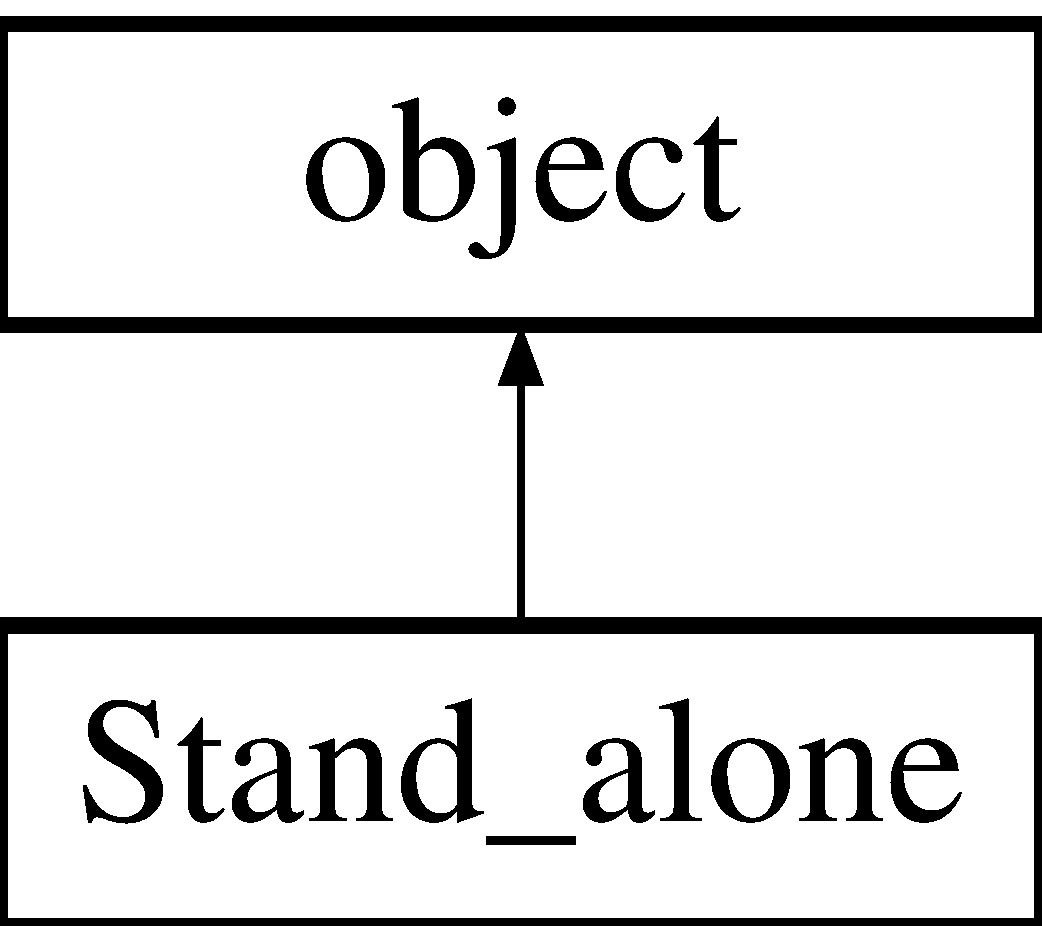
\includegraphics[height=2.000000cm]{classopenbu_1_1standalone_1_1_stand__alone}
\end{center}
\end{figure}
\subsection*{Public Member Functions}
\subsection*{Public Attributes}
\subsection*{Private Attributes}


The documentation for this class was generated from the following file\+:\begin{DoxyCompactItemize}
\item 
/\+Users/mouginot/work/app/\+Open\+B\+U/openbu/standalone.\+py\end{DoxyCompactItemize}

\hypertarget{classopenbu_1_1sequence_1_1_step__0}{}\section{Step\+\_\+0 Class Reference}
\label{classopenbu_1_1sequence_1_1_step__0}\index{Step\+\_\+0@{Step\+\_\+0}}
Inheritance diagram for Step\+\_\+0\+:\begin{figure}[H]
\begin{center}
\leavevmode
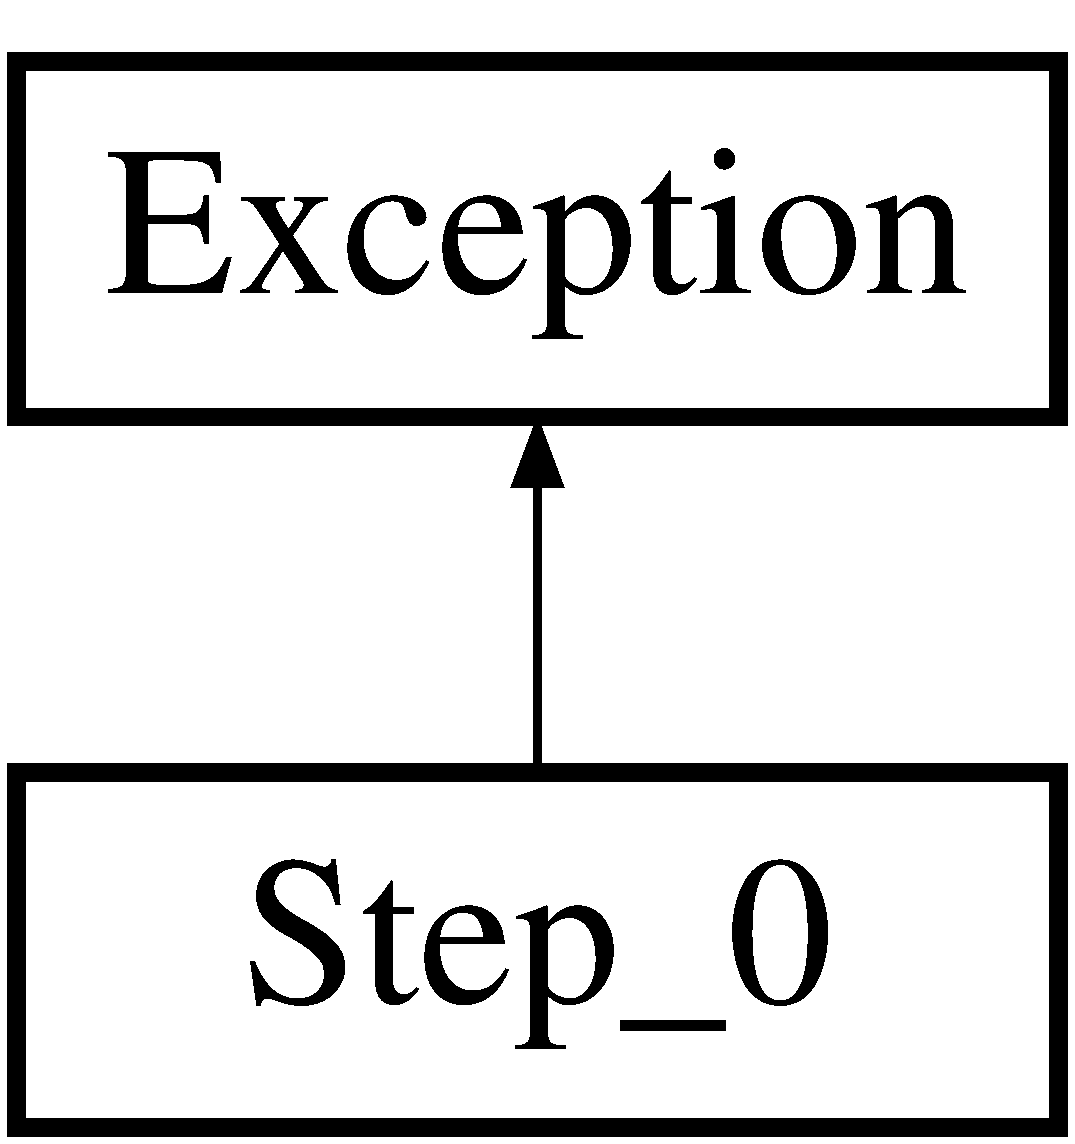
\includegraphics[height=2.000000cm]{classopenbu_1_1sequence_1_1_step__0}
\end{center}
\end{figure}


\subsection{Detailed Description}
\begin{DoxyVerb}Raise when the user try to access subinterval for the first step\end{DoxyVerb}
 

The documentation for this class was generated from the following file\+:\begin{DoxyCompactItemize}
\item 
/\+Users/mouginot/work/app/\+Open\+B\+U/openbu/sequence.\+py\end{DoxyCompactItemize}

\hypertarget{classopenbu_1_1couple_1_1couple__openmc_1_1_s_t_o_p}{}\section{S\+T\+OP Class Reference}
\label{classopenbu_1_1couple_1_1couple__openmc_1_1_s_t_o_p}\index{S\+T\+OP@{S\+T\+OP}}
Inheritance diagram for S\+T\+OP\+:\begin{figure}[H]
\begin{center}
\leavevmode
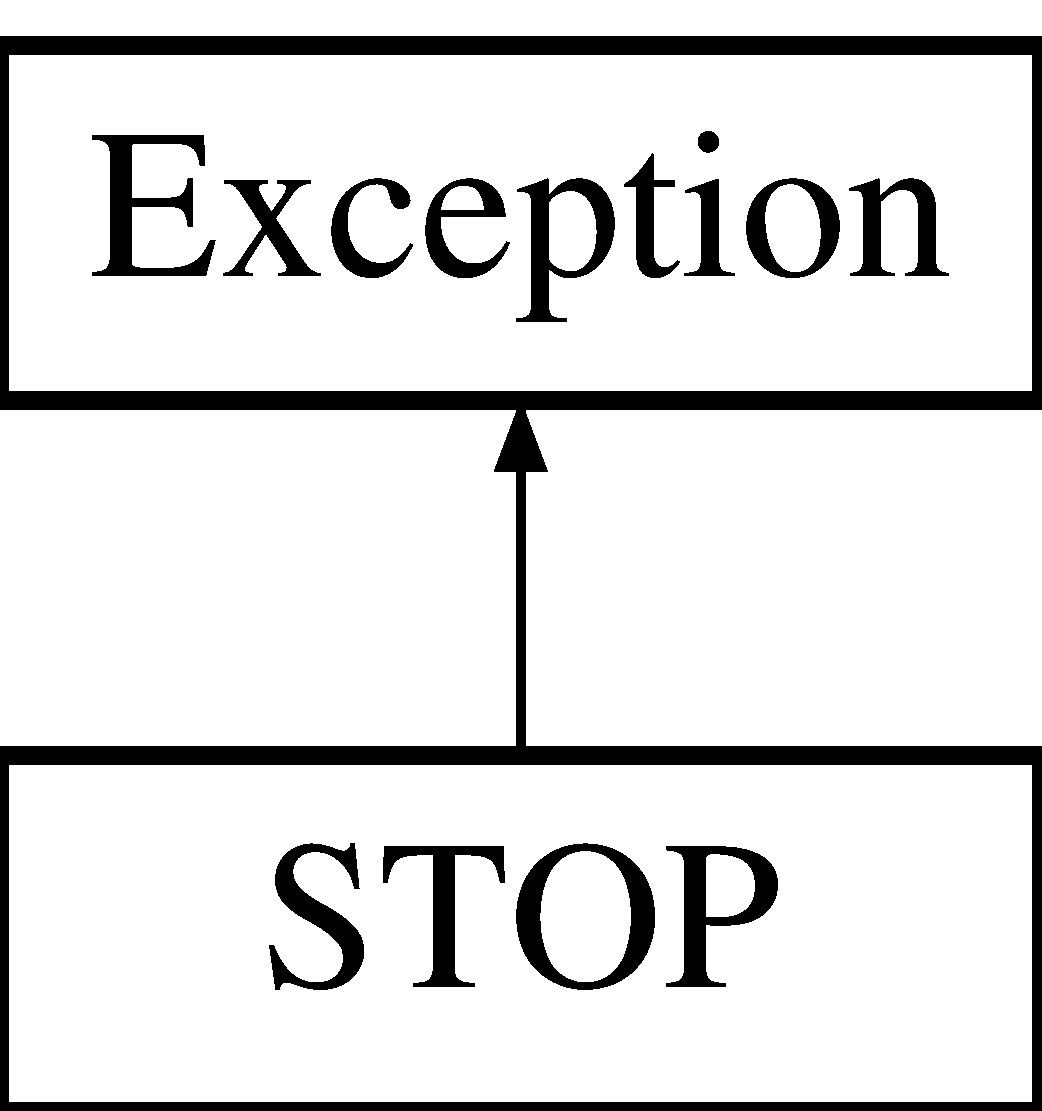
\includegraphics[height=2.000000cm]{classopenbu_1_1couple_1_1couple__openmc_1_1_s_t_o_p}
\end{center}
\end{figure}


\subsection{Detailed Description}
\begin{DoxyVerb}Just a way to stop the code\end{DoxyVerb}
 

The documentation for this class was generated from the following file\+:\begin{DoxyCompactItemize}
\item 
/\+Users/mouginot/work/app/\+Open\+B\+U/openbu/couple/\mbox{\hyperlink{couple__openmc_8py}{couple\+\_\+openmc.\+py}}\end{DoxyCompactItemize}

\hypertarget{classopenbu_1_1system_1_1_system}{}\section{System Class Reference}
\label{classopenbu_1_1system_1_1_system}\index{System@{System}}
Inheritance diagram for System\+:\begin{figure}[H]
\begin{center}
\leavevmode
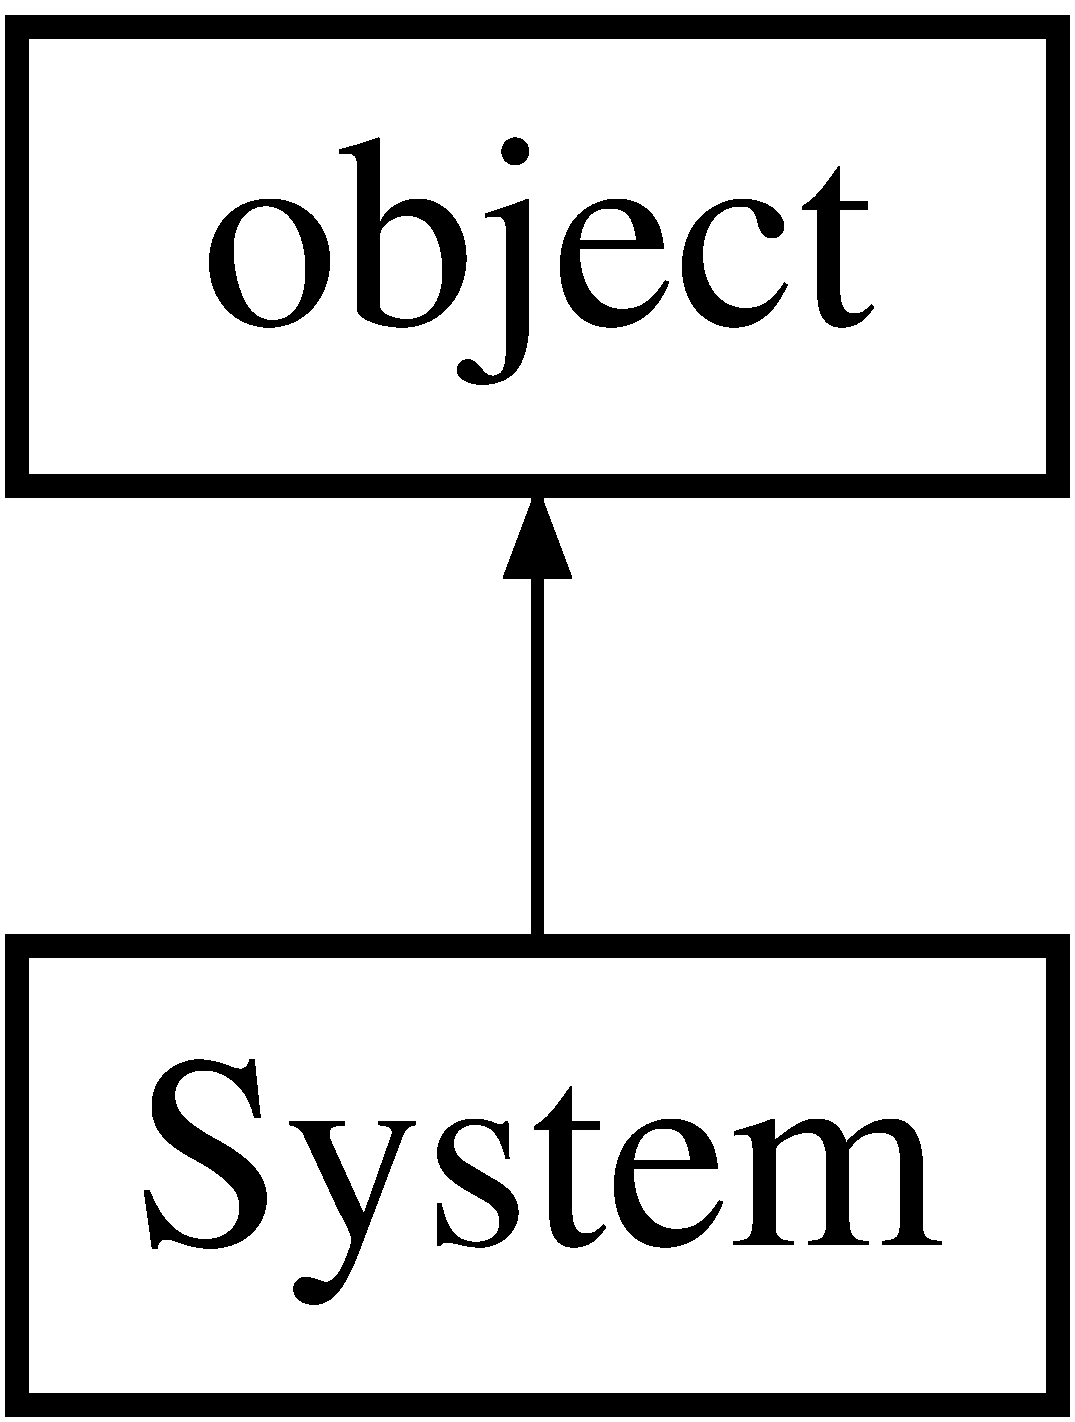
\includegraphics[height=2.000000cm]{classopenbu_1_1system_1_1_system}
\end{center}
\end{figure}
\subsection*{Public Member Functions}
\subsection*{Public Attributes}
\subsection*{Private Member Functions}
\subsection*{Private Attributes}


The documentation for this class was generated from the following file\+:\begin{DoxyCompactItemize}
\item 
/\+Users/mouginot/work/app/\+Open\+B\+U/openbu/system.\+py\end{DoxyCompactItemize}

\hypertarget{classopenbu_1_1utils_1_1reactions__class_1_1xs__lib}{}\section{xs\+\_\+lib Class Reference}
\label{classopenbu_1_1utils_1_1reactions__class_1_1xs__lib}\index{xs\+\_\+lib@{xs\+\_\+lib}}
Inheritance diagram for xs\+\_\+lib\+:\begin{figure}[H]
\begin{center}
\leavevmode
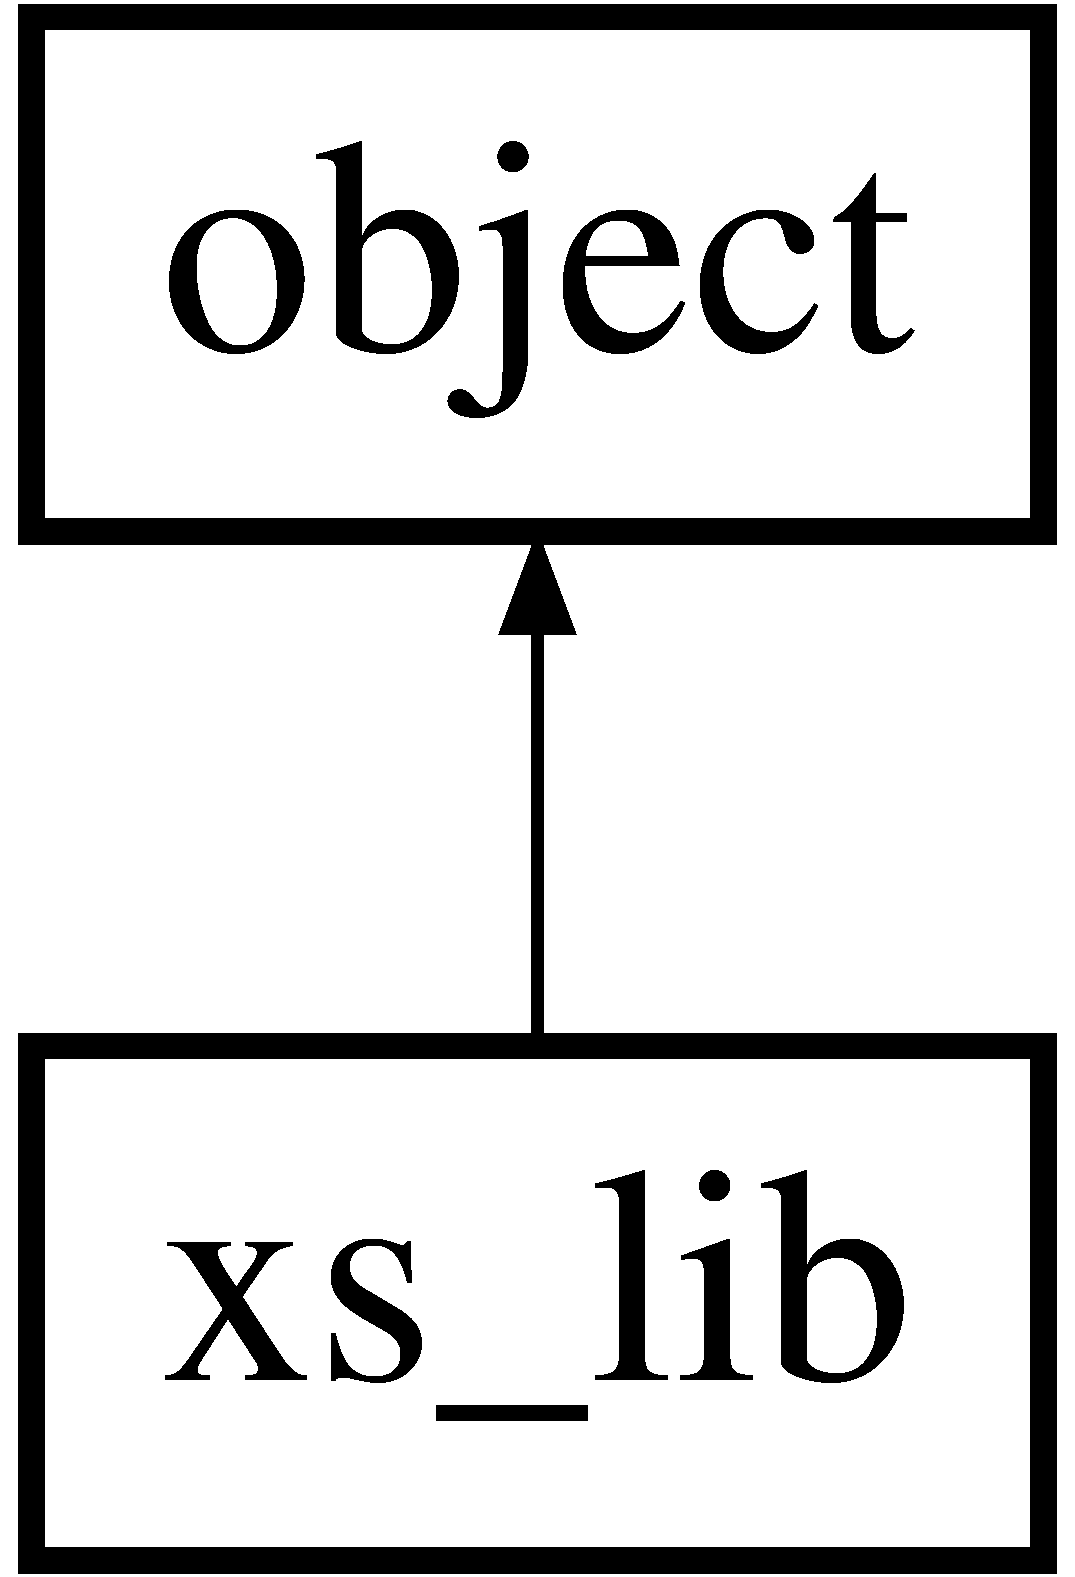
\includegraphics[height=2.000000cm]{classopenbu_1_1utils_1_1reactions__class_1_1xs__lib}
\end{center}
\end{figure}
\subsection*{Public Member Functions}
\subsection*{Private Attributes}


The documentation for this class was generated from the following file\+:\begin{DoxyCompactItemize}
\item 
/\+Users/mouginot/work/app/\+Open\+B\+U/openbu/utils/reactions\+\_\+class.\+py\end{DoxyCompactItemize}

\hypertarget{classopenbu_1_1utils_1_1data__processor_1_1xs__name__not__found}{}\doxysection{xs\+\_\+name\+\_\+not\+\_\+found Class Reference}
\label{classopenbu_1_1utils_1_1data__processor_1_1xs__name__not__found}\index{xs\_name\_not\_found@{xs\_name\_not\_found}}
Inheritance diagram for xs\+\_\+name\+\_\+not\+\_\+found\+:\begin{figure}[H]
\begin{center}
\leavevmode
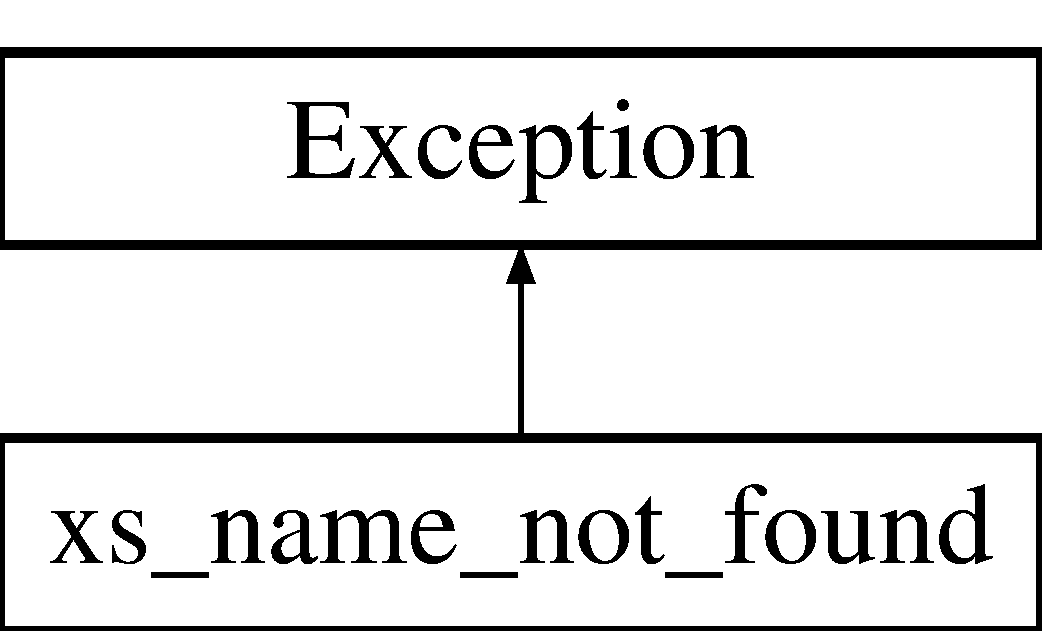
\includegraphics[height=2.000000cm]{classopenbu_1_1utils_1_1data__processor_1_1xs__name__not__found}
\end{center}
\end{figure}


\doxysubsection{Detailed Description}
\begin{DoxyVerb}Raise when the user tries to access fission XS for a nuclide which fission XS have not been set yet \end{DoxyVerb}
 

The documentation for this class was generated from the following file\+:\begin{DoxyCompactItemize}
\item 
utils/data\+\_\+processor.\+py\end{DoxyCompactItemize}

\hypertarget{classopenbu_1_1passport_1_1_x_s__not__yet__set}{}\doxysection{X\+S\+\_\+not\+\_\+yet\+\_\+set Class Reference}
\label{classopenbu_1_1passport_1_1_x_s__not__yet__set}\index{XS\_not\_yet\_set@{XS\_not\_yet\_set}}
Inheritance diagram for X\+S\+\_\+not\+\_\+yet\+\_\+set\+:\begin{figure}[H]
\begin{center}
\leavevmode
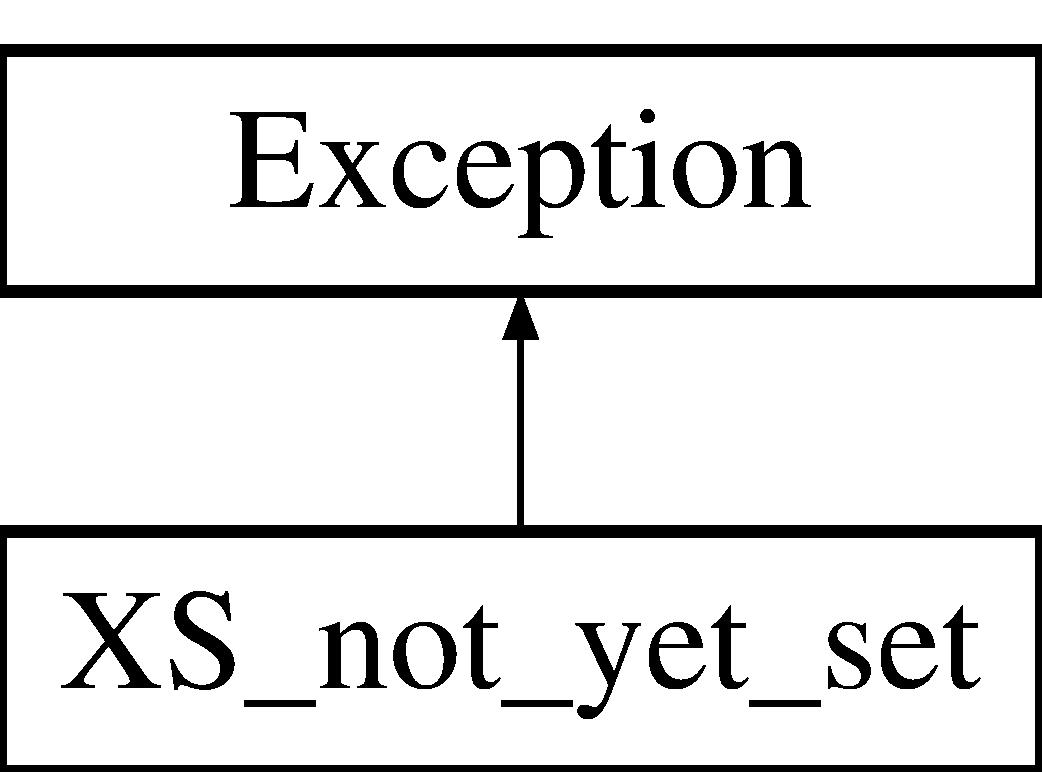
\includegraphics[height=2.000000cm]{classopenbu_1_1passport_1_1_x_s__not__yet__set}
\end{center}
\end{figure}


\doxysubsection{Detailed Description}
\begin{DoxyVerb}Raise when the user tries to access XS for a nuclide which XS have not been set yet \end{DoxyVerb}
 

The documentation for this class was generated from the following file\+:\begin{DoxyCompactItemize}
\item 
passport.\+py\end{DoxyCompactItemize}

%--- End generated contents ---

% Index
\backmatter
\newpage
\phantomsection
\clearemptydoublepage
\addcontentsline{toc}{chapter}{Index}
\printindex

\end{document}
